\documentclass[dvipdfmx]{ampbt}
%% compile: platex thesis.tex && bibtex thesis && platex thesis.tex && platex thesis.tex && dvipdfmx thesis.dvi

%% クラスオプション:
%% chapter:   \chapterコマンドを使用可能にする(jsbook (report) を使う).
%% duplexing: 両面印刷用の PDF を出力する.
%% その他 jsclasses に指定可能なオプションが指定できます(そのまま渡される).

%% 報告書の題目 %%%%%%%%%%%%%%%%%%%%%%%%%%%%%%%%%%%%%%%%%%%%%%%%%%%%%%%%%%%%%%%%%
\title{Friend-to-friendネットワークにおける} % 題目1行目
      {効率的な分散ルーティング}                         % 題目2行目
      {}                                         % 題目3行目
%% 指導教員 %%%%%%%%%%%%%%%%%%%%%%%%%%%%%%%%%%%%%%%%%%%%%%%%%%%%%%%%%%%%%%%%%%%%%
\supervisors{宮崎修次}{講師}    % 指導教員1人目 {氏名}{職名}
            {}{}    % 指導教員2人目 {氏名}{職名}
            {}{}                % 指導教員3人目 {氏名}{職名}
%% 入学年月 %%%%%%%%%%%%%%%%%%%%%%%%%%%%%%%%%%%%%%%%%%%%%%%%%%%%%%%%%%%%%%%%%%%%%
\entrancedate{24}{4}            % {年(平成)}{月}
%% 著者氏名 %%%%%%%%%%%%%%%%%%%%%%%%%%%%%%%%%%%%%%%%%%%%%%%%%%%%%%%%%%%%%%%%%%%%%
\author{高橋}{彰}             % {姓}{名}
%% 提出日 %%%%%%%%%%%%%%%%%%%%%%%%%%%%%%%%%%%%%%%%%%%%%%%%%%%%%%%%%%%%%%%%%%%%%%%
\submissiondate{29}{1}{XX}      % {年(平成)}{月}{日}
%% 提出年度 %%%%%%%%%%%%%%%%%%%%%%%%%%%%%%%%%%%%%%%%%%%%%%%%%%%%%%%%%%%%%%%%%%%%%
\submissionjay{28}              % {年度(平成)}
%% 摘要 %%%%%%%%%%%%%%%%%%%%%%%%%%%%%%%%%%%%%%%%%%%%%%%%%%%%%%%%%%%%%%%%%%%%%%%%%
\abstract{%
  本研究では, ネットワークトポロジーのスモール・ワールド性を利用し, 効率的かつ非中央集権的なルーティングを実現するための手法を提起する. 
}
%% パッケージの読み込みや自分用のマクロの定義 %%%%%%%%%%%%%%%%%%%%%%%%%%%%%%%%%%%
\usepackage{amsmath,amssymb, amsthm}
\usepackage{enumitem}
\usepackage{bm}
\usepackage{type1cm}
\usepackage{ascmac} % for box
\usepackage{hyperref}
\usepackage{url}
\usepackage[xindy]{glossaries}
\usepackage{algorithm}
\usepackage{algpseudocode}
\usepackage[justification=centering]{caption}
\usepackage{subcaption}
\usepackage{graphicx}
%\usepackage{algorithm2e}
%\parindent = 0pt
\makeatletter
\makeatother
\newcommand{\argmax}{\mathop{\rm arg~max}\limits}
\newcommand{\argmin}{\mathop{\rm arg~min}\limits}
\newcommand{\rme}{\mathrm{e}}

%% term list
\makeglossaries
\newacronym{f2f}{F2F}{Friend-to-friend}
\newacronym{wot}{WoT}{Web of Trust}
\newglossaryentry{localcon}
{
    name={local contact},
    description={距離空間上に配置されたグラフにおいて最も近距離にあるノード間を接続するエッジ}
}
\newglossaryentry{darknet}
{
    name={Darknet},
    description={Friend-to-friendと同義}
}
\newglossaryentry{deadend}
{
    name={dead-end},
    description={メッセージを受け取ったノードが自分自身よりもターゲットに近い隣接ノードを持たない状態}
}
\newglossaryentry{embedding}
{
    name={埋め込み},
    description={TBD}
}
\newglossaryentry{swap}
{
    name={SWAP},
    description={TBD}
}
\newglossaryentry{id}
{
    name={ID},
    description={TBD}
}
\newglossaryentry{coord}
{
    name={座標},
    description={TBD}
}
\newglossaryentry{gremb}
{
    name={Greedy embedding},
    description={TBD}
}




%% 出力の制御 %%%%%%%%%%%%%%%%%%%%%%%%%%%%%%%%%%%%%%%%%%%%%%%%%%%%%%%%%%%%%%%%%%%

%% 本文を出力しない場合,次の行をコメントアウトして下さい.
% \outputbodyfalse

%% 末尾に表紙,背表紙を出力しない場合,次の行をコメントアウトして下さい.
% \outputcoverfalse

%% 末尾に提出用摘要を出力しない場合,次の行をコメントアウトして下さい.
% \outputabstractforsubmissionfalse

%% ampbt.cls では表紙等の作成のために geometry パッケージを使用しているため,本文
%% のレイアウトを変えるために \usepackage[...]{geometry} とすると Option clash が
%% 発生します.何らかの理由で本文のレイアウトを変更したい場合は \geometry{...} を
%% 使用して下さい.
%% また,jsclasses を使用しているため,例えば 3cm を指定したい場合は 3truecm と書
%% く必要があります.
% \geometry{hmargin=3truecm,vmargin=2truecm}

\begin{document}
\ifoutputbody
%% 中表紙,摘要,目次 %%%%%%%%%%%%%%%%%%%%%%%%%%%%%%%%%%%%%%%%%%%%%%%%%%%%%%%%%%%
\makeinsidecover                % 中表紙
\makeabstract                   % 摘要
\maketoc                        % 目次
\setcounter{page}{1}            % 本文のページ番号を1から始める
%% 本文 %%%%%%%%%%%%%%%%%%%%%%%%%%%%%%%%%%%%%%%%%%%%%%%%%%%%%%%%%%%%%%%%%%%%%%%%%
\section{序論}
近年インターネットを介したコミュニケーションまたは出版は, 我々の生活において大きな位置を占めるようになってきた. それに伴いユーザーのプライバシー保護を重視したコミュニケーションツールの実装に対する需要が非常に高まっている. その要因として, 例えば近年ではエドワード・スノーデンによって公に明らかにされたアメリカ国家安全保障局(NSA)による大規模な大衆監視が挙げられる.

特定の企業や団体が中央集権的に管理する情報共有方式はこのような監視・漏洩のリスクが高いため, 非中央集権的な情報共有を実現するためのアプローチとしてP2P方式が頻繁に採用される. P2Pは中心的な管理者を持たない分散的なオーバーレイネットワークであり, 一般的なクライアント-サーバー方式と比較して負荷分散, スケーラビリティ, 匿名性, 耐障害性等の点で優れている\cite{lua2005survey}. そしてP2P方式の中でも特にピアの匿名性・プライバシー保護を重視したものはF2F(friend-to-friend)\cite{bricklin2000friend}ネットワークと呼ばれる. F2F方式においてネットワーク上の各ノードは, 信頼のおける特定ノードとのみ通信するため, Chord\cite{stoica2001chord}などの分散ハッシュテーブル(DHT)方式とは異なり, ソフトウェアによって動的にネットワーク構造を最適化することはできず, ネットワーク構造は常に現実の信頼関係ネットワークの部分グラフに対応する. そしてネットワーク上で隣接していないノード同士がデータの送受信を行うためにはいずれかのノードが「知り合いの知り合い」を辿って他方のノードに到達するための経路を探索する必要性が生じる\cite{roos2016dealing}.

F2Fオーバーレイネットワークの最も代表的な実装例は, Freenet\cite{clarke2001freenet}のF2Fモード\cite{clarke2010private}であり, 基本的なプロトコルはSandberg\cite{sandberg2006distributed}が2006年に提案した手法に基づいている. Freenetでは, 信頼関係のネットワークがスモールワールド性を持つと仮定し, 単純なgreedyルーティング (各ノードは隣接ノード中, 最もターゲットに近いノードを次ノードとして選択) により, $O(\log^2 n)$のホップ数でルーティングを可能にするKleinbergのスモールワールドネットワークモデル\cite{kleinberg2000small}に基づいている.

ただしFreenetには未だ様々な問題点が残っている. 第一にSandbergが提案した手法では, Kleinbergモデルが依拠している「格子上で最も近距離にいるノード同士は必ずエッジを持つ」という仮定を決定論的に満たすことができないため, Freenetの実装においてはgreedyルーティングの代わりにdistance-directed depth-first search ($D^2$-$DFS$)が採用されている. しかしこの$D^2$-$DFS$アルゴリズムが特定の条件下において$O(\log^2 n)$のホップ数を達成することができないことはRoos, Strufeらにより解析的に証明された\cite{roos2012provable}\cite{roos2016dealing}\cite{roos2016analyzing}. またFreenetでは, ノードへのID割り当てアルゴリズムの一環としてノード同士がIDを交換するが, この際悪意のあるノードが虚偽のID報告を繰り返すことにより, ノードがID空間上に偏在し, 結果的にルーティングの効率性が低下するというPitch black attack\cite{evans2007routing}などの深刻な脆弱性が指摘されている. よってFreenetのF2Fモードは効率性や頑健性の面で問題点が残り, 現在もそれらを解決するための研究が続けられている.

本研究では, 以上に挙げられたFreenetの問題点のうちルーティングの効率性に着目する. 今回我々は{\c{S}}im{\c{s}}ek, Jensenらによって提案されたルーティングアルゴリズム, expected-value navigation (EVN)\cite{simsek2008navigating}をFreenetプロトコルに適用可能な形に修正することにより, スケールフリー性を持った\acrshort{f2f}ネットワークにおいて既存ルーティングアルゴリズムよりも高いパフォーマンスを発揮する$D^3$-$DFS$を提案する. また, 先行研究のシミュレーション実験においてはルーティングの成功率が向上するように実データの恣意的な改変が施されていたが, 本研究では改変を施さない実データに対するシミュレーション実験を行うことにより, 現実の\acrshort{f2f}トポロジーにより近いネットワークにおけるルーティングアルゴリズムのパフォーマンス評価を行った.

 \section{先行研究}
   \subsection{Kleinbergモデル} \label{sec:kleinberg}
   KleinbergはMilgramのスモールワールド実験において個々人が友人関係ネットワークの全体像を知らず, ターゲットの住所, 職業と各自の友人の住所という限られた情報のみを用いたにも関わらず, 短いホップ数でターゲットまで手紙を届けることができたことに着想を得て, 分散的(decentralized)なルーティングが効率的となるようなスモールワールドネットワークモデルを提唱した\cite{kleinberg2000small}.

   Kleinbergのスモールワールドネットワークモデルは以下の手順で生成されるグラフのクラス$K(n,m,p,q,r)$として定義される. ただし$p \geq 1, q \geq 0, r \geq 0$とする. 
   \begin{enumerate}
    \item $m$次元格子上に配置された$n^m$個のノードを初期状態とする.
    \item 各ノードは格子上で自分から格子距離$p$以内にある全てのノードとの短距離エッジ (local contact) を得る.
    \item 各ノード$u$は$q$本の長距離エッジ (long-range contact)を追加する. ただし$u$が$v$とのエッジを持つ確率を$p(u,v)$として,
	  \begin{eqnarray}
	   p(u,v)=\cfrac{1}{d(u,v)^{r}Z} \label{eq:kleinberg_p}
	  \end{eqnarray}
   \end{enumerate}
   ここで, 
   \begin{itemize}
    \item  $r$: 他ノードとの接続確率がどの程度格子距離に依存するかを示すパラメータ
    \item  $d(u,v)$: $u,v$間の格子距離 (例: 2次元格子であれば$d(u,v)=|u_x - v_x| + |u_y - v_y|$)
    \item $Z = \displaystyle \sum_{v\in V, v\neq u}^{}d(u,v)^{-r}$: 正規化定数
   \end{itemize}
   である. このモデルは「距離が近い人どうしほど知りあいである確率が高い」という非常に直観的な発想に基づいている. なお$r=0$の場合はWatts-Strogatzモデルと同等となる. Kleinbergモデルのアルゴリズムにより生成されたグラフを図\ref{fig:kleinberg}に示す. (a)は2次元格子, (b)は1次元格子の場合である.
   \begin{figure}[htbp]
    \centering
    \begin{subfigure}[b]{0.48\textwidth}
        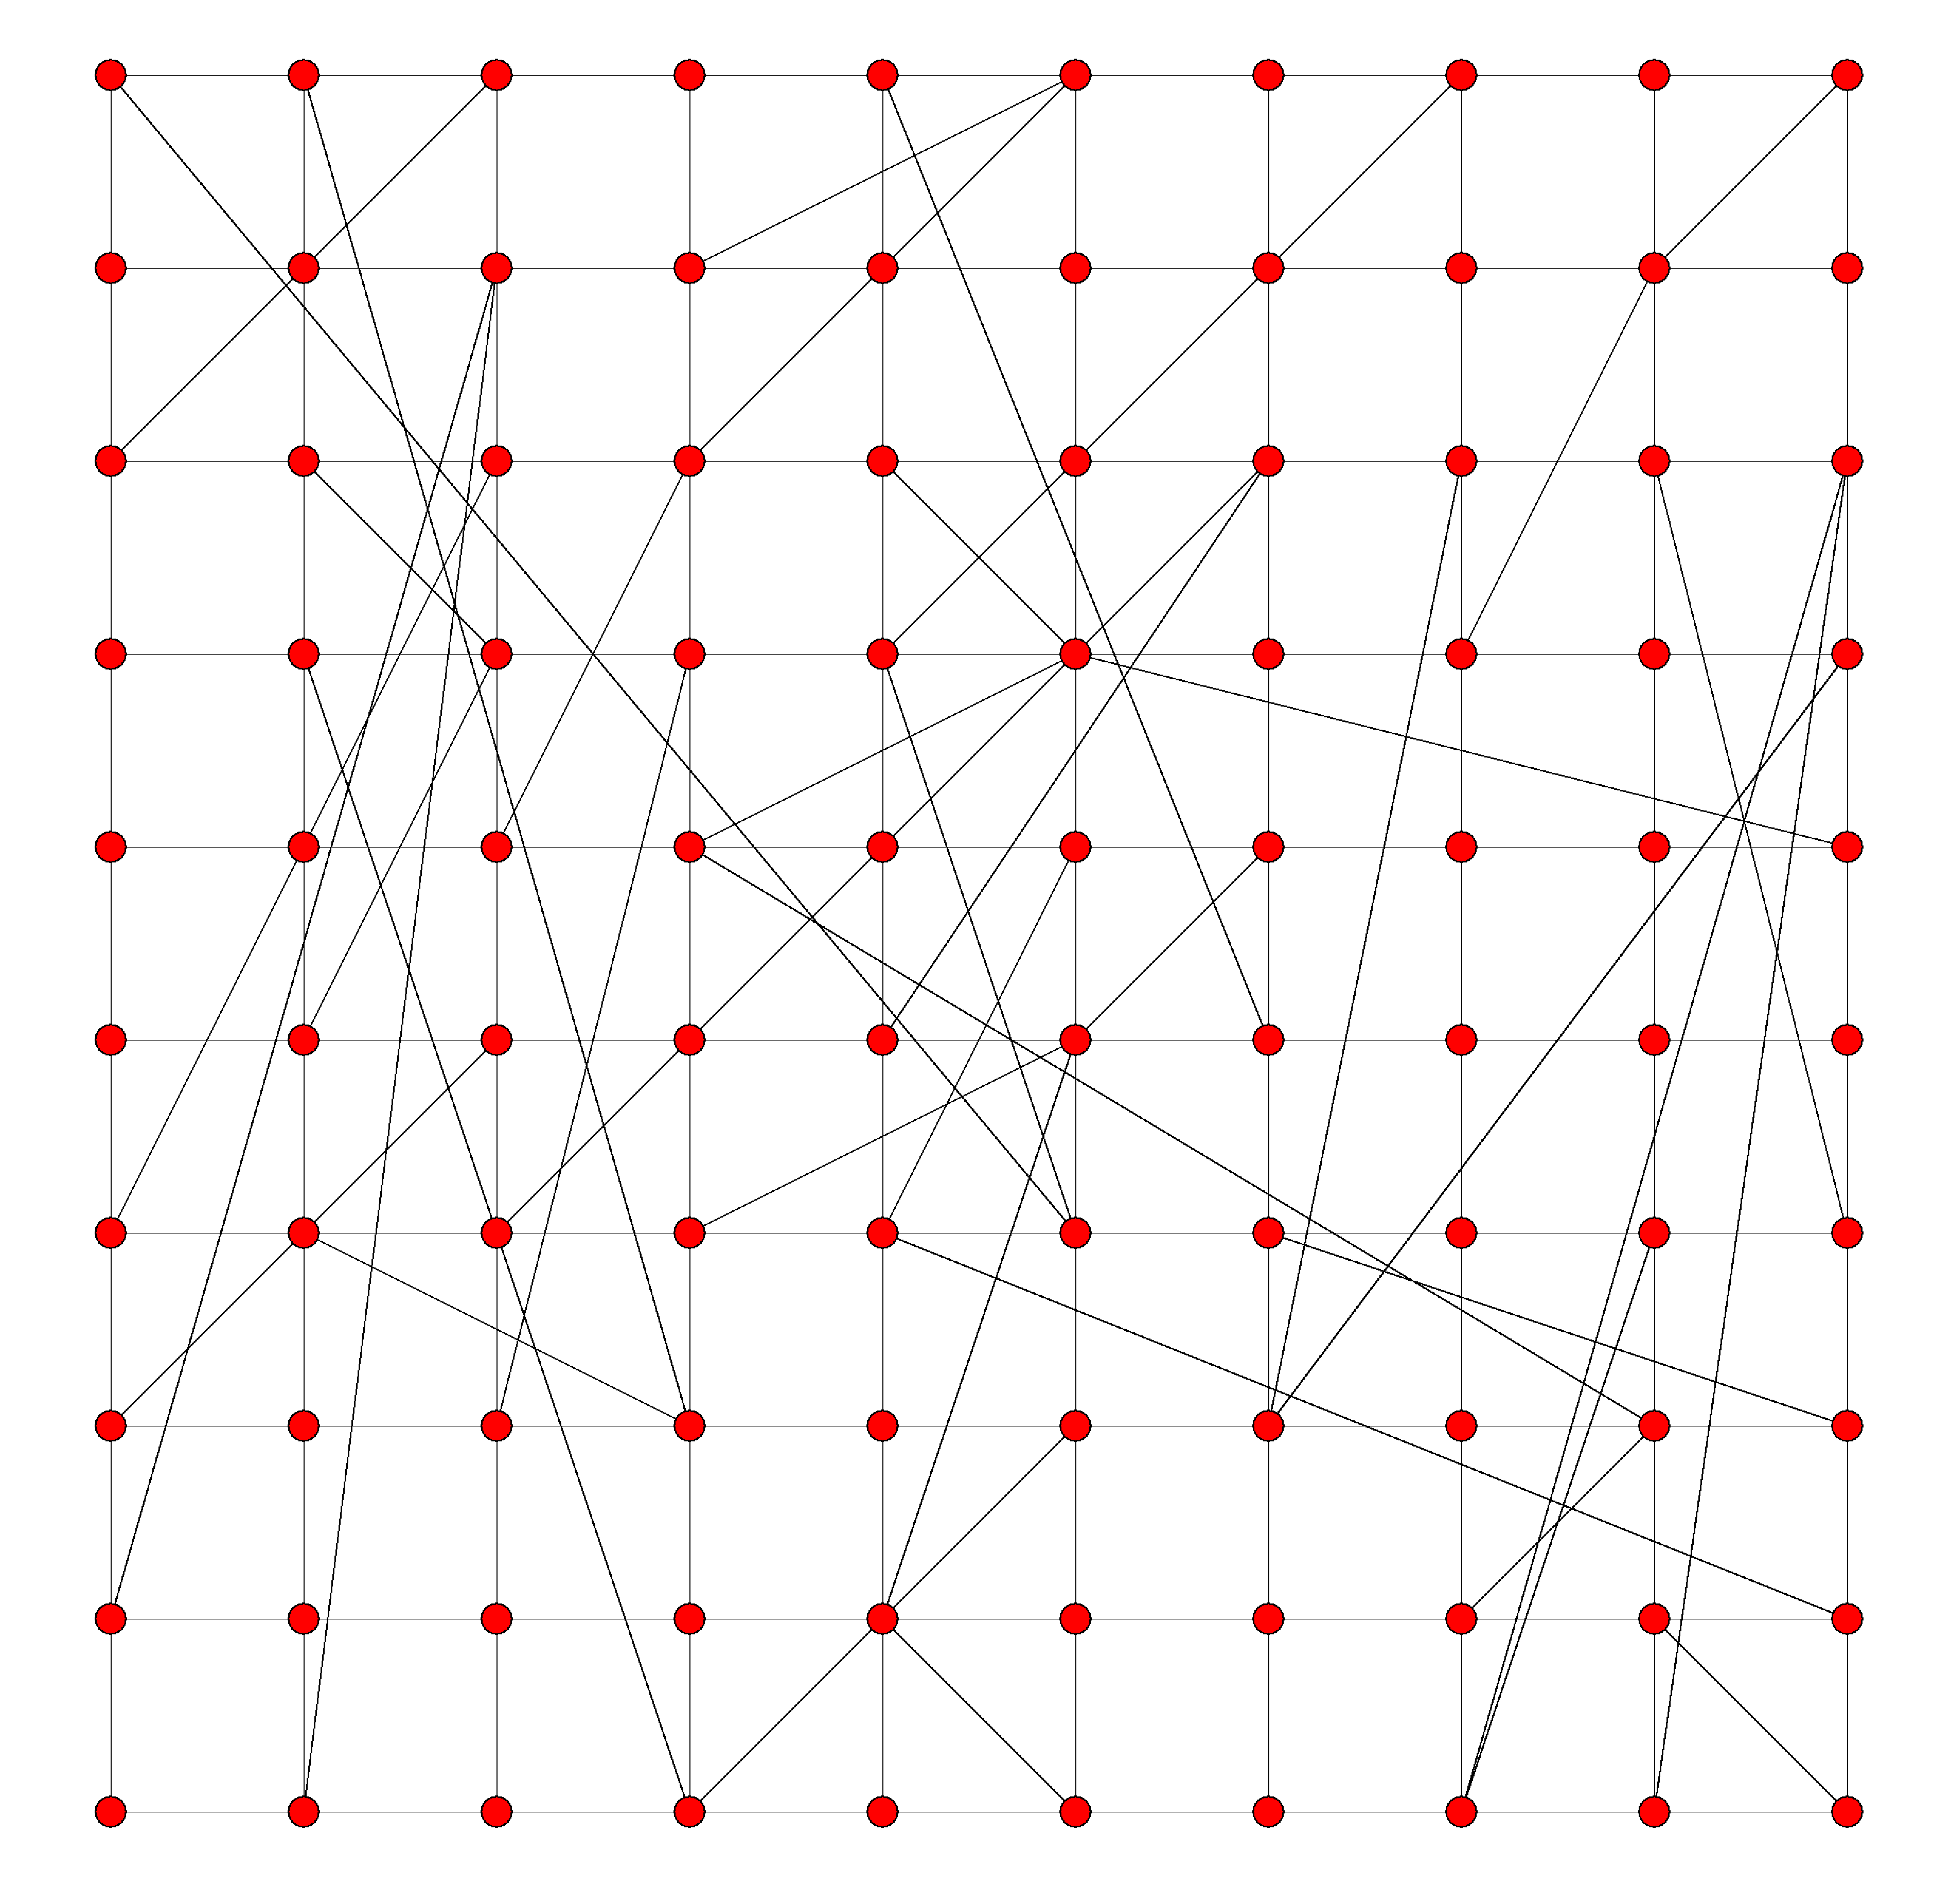
\includegraphics[width=\textwidth]{../fig/kleinberg_2dim.eps}
     \caption{$n=10,m=2,p=1,q=1,r=2$}
    \end{subfigure}
    \begin{subfigure}[b]{0.48\textwidth}
        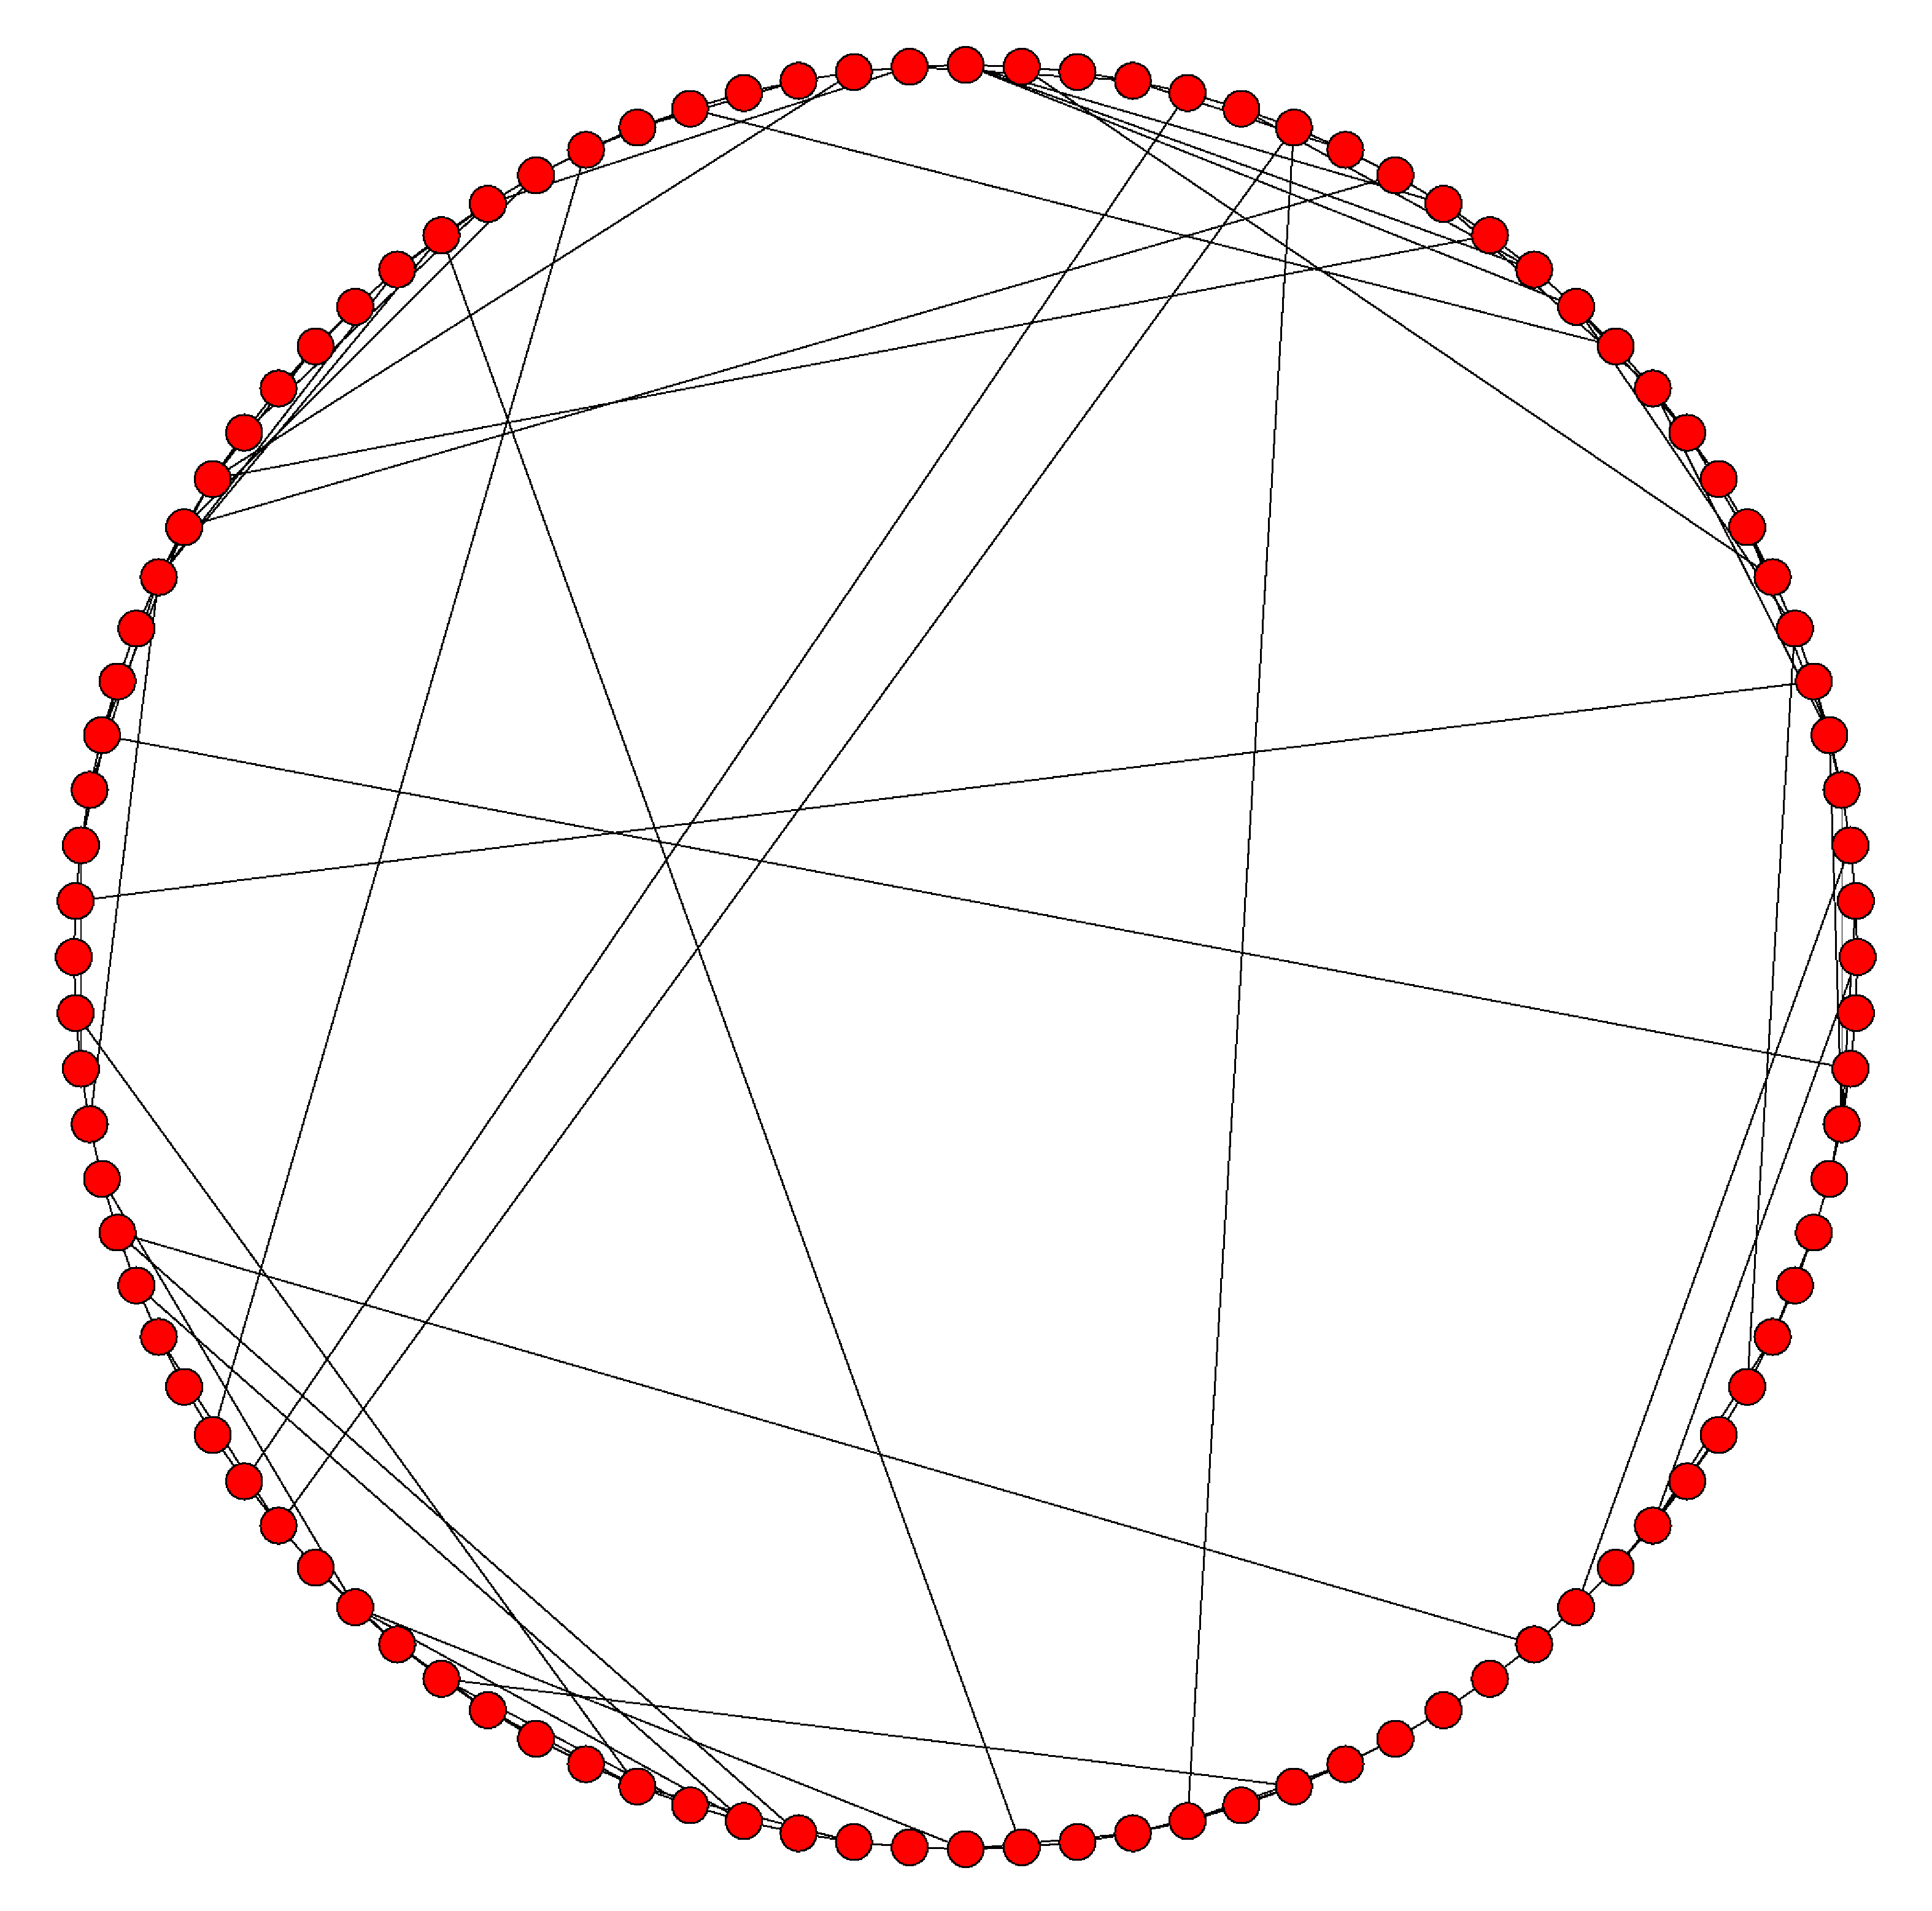
\includegraphics[width=\textwidth]{../fig/kleinberg_1dim.eps}
        \caption{$n=100,m=1,p=1,q=1,r=1$}
    \end{subfigure}
    \caption{Kleinbergのスモールワールドネットワーク}
    \label{fig:kleinberg}
   \end{figure}

   このようにして生成されたグラフにおいて, Kleinbergは$r=m$の場合, つまり格子次元にパラメータが一致する場合に, greedyルーティングによる任意のノードからターゲットまでのホップ数期待値が$O(\log^2n)$となることを証明した. ここでgreedyルーティングとは「各ノードはターゲットまでの距離が最も近い隣接ノードにメッセージをフォワードする」というアルゴリズムを意味し, 各ノードは自分, 隣接ノード, ターゲットの座標という限られた情報のみを用いて次ノード選択の意思決定を行うため, greedyルーティングは分散的である.


   \subsection{Freenetプロトコル: 埋め込みとルーティング} \label{sec:freenetprotocols}
   この節ではFreenetのF2Fモード(またはDarknetモードとも呼ばれる)の概略について述べる. F2Fモードの目的はP2Pシステムにおけるノードのプライバシー保護であり, ネットワーク上の各ノードは予め信頼のおけるノードとのみ直接の通信を行う. つまり「友人と友人」(friend-to-friend)の通信のみを行うという制約を設けることによって, 信頼関係の外部にいる攻撃者によるプライバシー侵害を困難にしようというのが核心となるコンセプトである.

   この制約があるため, F2Fモードにおいては通信効率を最適化するようにネットワークトポロジー自体に変更を加えることが不可能であり, 各ノードはネットワークの全体像も把握することができない. よって, ネットワーク上で隣接していないノードどうしがデータの送受信を行うためには, Milgramの実験と同様にネットワーク上の中継ノードが局所的な情報をのみを用いてメッセージのフォワーディングを繰り返す必要がある. 

   そこでネットワークトポロジーを変えずにルーティングを効率化するためにF2Fモードが取るアプローチが, ネットワークのID空間への「埋め込み」(embedding)である. 埋め込みとルーティングの概念図を図\ref{fig:f2f_overview}に示す.

   \begin{figure}[htbp]
    \centerline{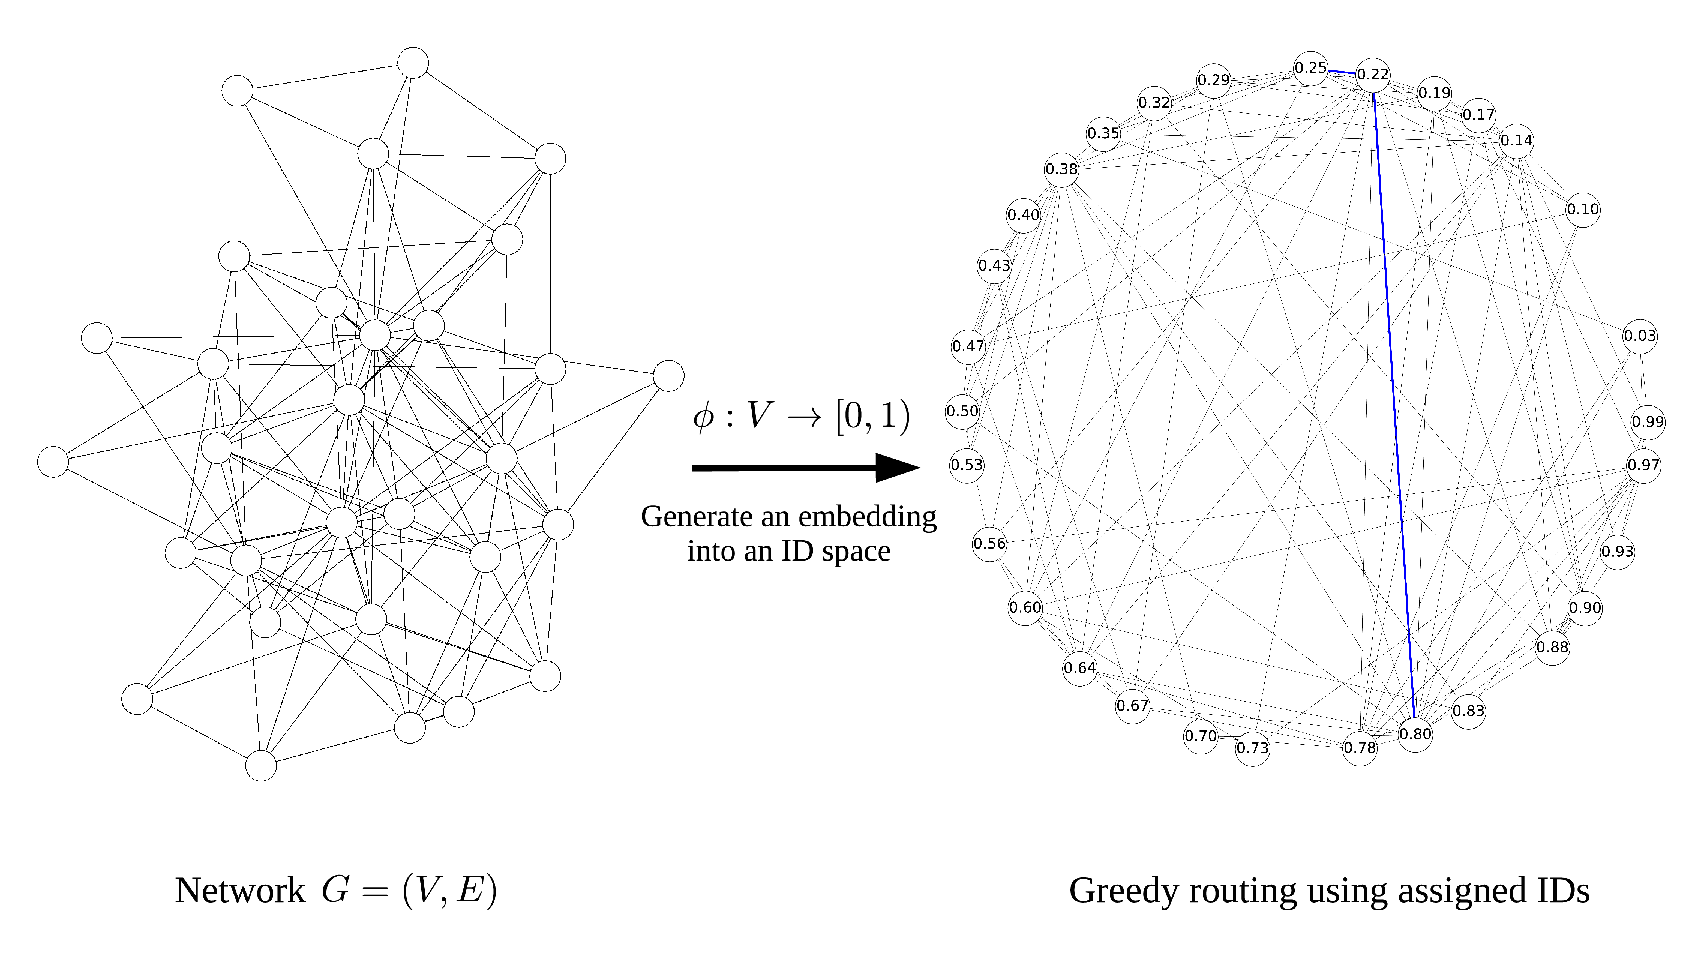
\includegraphics[width=150mm]{../fig/greedy_embedding_overview.eps}}
    \caption{F2Fネットワークにおける埋め込みとルーティングの概略}
    \label{fig:f2f_overview}
   \end{figure}

   一般的にネットワーク$G=(V,E)$の距離空間$(X,d)$への埋め込みは単射$\phi:V \to X$で定義される\cite{papadimitriou2005conjecture}. Freenetでは以下の式(\ref{eq:f2f_dist})で定義される距離関数$d$を備えた単位区間$[0,1)$が上記の$X$に対応し, ID空間(ID space)またはキー空間(key space)などと呼ばれる. 以下では空間上の一点を便宜的に''ID''または「座標」と呼ぶこととする. 図\ref{fig:f2f_overview}のようにID空間上の各点は円上の点に, 2点間の距離は円周上の距離に対応付けることができる.

   \begin{eqnarray}
    \forall x,y \in [0,1), d(x,y) = \min\{|x-y|, 1 - |x-y|]\} \label{eq:f2f_dist}
   \end{eqnarray}

   よってF2Fモードでは, 効率的な分散ルーティングが可能となるようにID空間への埋め込み$\phi$を生成することが重要となる. 

   \subsubsection{埋め込みの生成: SWAPアルゴリズム}
   さてF2Fモードの埋め込みの生成はSandbergが2006年に提案した手法(以下SWAPアルゴリズムと呼ぶ)に基づいている\cite{sandberg2006distributed}. SWAPアルゴリズムは埋め込みの生成をパラメータ$\phi$の推定問題としてみなし, ID空間に埋め込まれたグラフがKleinbergモデルによって生起する確率が高くなるように(つまり隣接するノード間のID空間における距離の分布が式(\ref{eq:kleinberg_p})に従うように), $\phi$をMetropolis-Hastings法によりサンプリングする.

   SWAPアルゴリズムの概略は以下の通り.
   \begin{enumerate}
    \item ノード$u$はID交換相手の候補$v$をネットワーク上でのランダムウォークにより選択し, ID交換リクエストを送る.
    \item 各$u,v$がそれぞれ「隣接ノードと自分の距離」「隣接ノードと相手の距離」を計算することで, 以下の採択率$\beta(\phi_1, \phi_2)$を得る. 
    \begin{eqnarray}
     \beta(\phi_1, \phi_2)= \min \left[1, \frac{\prod_{w \in N(u)}d(\phi_1(w), \phi_1(u))\prod_{w \in N(v)}d(\phi_1(w), \phi_1(v))}{\prod_{w \in N(u)}d(\phi_2(w), \phi_2(u))\prod_{w \in N(v)}d(\phi_2(w), \phi_2(v))}\right] \label{eq:acceptance}
    \end{eqnarray}
	  ただし$N(u), N(v)$は$u,v$の隣接ノード集合, $\phi_1$は現在の埋め込みのサンプル, $\phi_2$は候補サンプルで, $\phi_1$における$u,v$のID割り当てを入れ替えたものである.
    \item $[0,1)$上の一様乱数を生成し乱数が$\beta(\phi_1, \phi_2)$を超えなければ, $u,v$はIDを交換, すなわち埋め込みの候補サンプル$\phi_2$を採択し, さもなくばID交換を行わない.
   \end{enumerate}

   なお採択確率$\beta(\phi_1,\phi_2)$の導出は, 付録に記述した.

   以上の操作を十分な回数反復することで, greedyルーティングによって短い平均ホップ数が達成できるようなIDの割り当てを生成することができる. Sandbergは人工的に生成したKleinbergのネットワークデータと実データに対してシミュレーション実験を行い, SWAPアルゴリズムの適用後割り当てられた座標情報が, ランダムに割り当てられた座標情報に比してgreedyルーティングの効率性を高めることを示した.

   \subsubsection{ルーティングアルゴリズム: $D^2$-$DFS$}
   SWAPアルゴリズムの適用は確かにgreedyルーティングの効率性を高めるようなIDの割り当てが可能であるが, 本来のKleinbergモデルと同様の$O(\log^2n)$のホップ数は保証されない. なぜなら, Kleinbergモデルでは全てのlocal contactが存在しているという仮定によってgreedyルーティングの最中にターゲットまでの距離が狭義に単調減少することが保証されているが, SWAPアルゴリズムによってID空間に埋め込まれたネットワークは必ずしもこのlocal contactを持たないからである. よって単純なgreedyルーティングでは''dead end''(自分よりもターゲットに近い隣接ノードが存在しない状態)に達してしまうため, SWAPアルゴリズムによって生成された埋め込みは''greedy embedding''ではない\footnote{任意の$u,t \in V, u\neq t$に対してある$v \in N(u)$が存在して$d(\phi(v), \phi(t)) < d(\phi(u), \phi(t))$を満たす時, 埋め込み$\phi:V \to X$は''greedy embedding''と呼ばれる. 詳細は\cite{papadimitriou2005conjecture}または\cite{kleinberg2007geographic}を参照.}. そこでFreenetではgreedyルーティングの代わりにホップ数上限付のdistance-directed depth-first search ($D^2$-$DFS$)を採用することでdead endに対処している. $D^2$-$DFS$ではgreedyルーティングと同じく「ターゲットに最も近い隣接ノード」にメッセージをフォワードすることを繰り返すが, 以下の2点において異なる.
   \begin{enumerate}
    \item dead-endに陥った場合でも, ルーティングを中断せず「ターゲットに最も近い隣接ノード」へメッセージをフォワードする. 
    \item 隣接ノードが全て訪問済みの場合, 自分に初めてメッセージを送ってきたノード(predecessor)にメッセージを戻す(backtrackingフェーズ).
    \item ホップ数が予め設定された上限に達した場合, もしくはソースノード(リクエストを発したノード)の隣接ノードが全て訪問済みの場合に限ってルーティング失敗とする.
   \end{enumerate}
   $D^2$-$DFS$の動作例を図\ref{fig:d2dfs_example}に示す.

   \begin{figure}[htbp]
    \centerline{\includegraphics[width=100mm]{../fig/d2dfs_example.png}}
    \caption{$D^2$-$DFS$の動作例: ソースノードID0.52, ターゲットノードID0.15の場合 \\ 赤い矢印はbacktrackingのフェーズを表している}
    \label{fig:d2dfs_example}
   \end{figure}

   Roos, Strufeらは埋め込みの不正確さを考慮してlocal contactの存在を仮定しないKleinbergのモデルを提案し, そのようなグラフにおいて$D^2$-$DFS$がポリ対数関数(polylogarithmic)のオーダーでルーティングを終えることができないことを解析的に証明した\cite{roos2013contribution}. 

   \subsection{EVN: Expected-value navigation} \label{sec:evn}
   {\c{S}}im{\c{s}}ek, Jensenらは2005年の論文でgreedyルーティングとは異なるルーティングアルゴリズムを提案し, スモールワールド性やスケールフリー性を持つ現実のネットワークにおいてgreedyルーティングよりも高いパフォーマンスを発揮することを実証的に示した\cite{simsek2005decentralized}. また続く2008年の論文では次ノード選択のヒューリスティックスを簡略化し, 分散的な実装が可能な形でアルゴリズムを提示した\cite{simsek2008navigating}. このルーティングアルゴリズムはexpected-value navigation(EVN)と呼ばれる.

   EVNの基本的なアイデアは, メッセージを持っているノード$u$の隣接ノード$v \in N(u)$からターゲットノード$t$までの経路長$l(v,t)$を考え, その期待値$E(l(v,t))$を近似的に計算し, $E(l(v,t))$を最小化するような$v$を次ノードとして選択するというものである. $E(l(v,t))$の2次以降の項を無視し, さらに二項分布をポアソン分布によって近似することにより以下のように簡略化が可能となる. ただし$k_v$を隣接ノード$v$の次数, $p(v,t)$を$v$から$t$へのエッジが生成される確率とする.
    \begin{eqnarray}
     E(l(v,t)) &=& \sum_i ip(l(v,t)=i)\nonumber \\
     &\approx& p(l(v,t)=1)  )\nonumber\\
     &=& 1- (1 - p(v,t))^{k_v} \nonumber\\
     &=& Binomial(0;  k_v, p(v,t)) \nonumber \\
     &\approx& 1 - Poisson(0; k_vp(v,t)) \nonumber\\
     &=& 1- e^{k_vp(v,t)} \label{eq:evn-basic}
    \end{eqnarray}
    よってある隣接ノード$v$が$E(l(v,t))$を最小化することは, $1/k_vp(v,t)$を最小化することと同値であるからヒューリスティック関数$f(v)$を
    \begin{eqnarray}
     f(v) = \frac{1}{k_vp(v,t)}\label{eq:evn-heuristic}
    \end{eqnarray}
    と定義すれば, 「メッセージを持つノード$u$は(\ref{eq:evn-heuristic})式で定義される$f(v)$を最小化するような隣接ノード$v \in N(u)$にメッセージをフォワードする」というシンプルなルーティングアルゴリズムにより, 「隣接ノード中ターゲットまでのホップ数が最も少ないと期待されるノード」を選択することができる. 



\section{問題設定}
\ref{sec:freenetprotocols}節に述べた\acrshort{f2f}ネットワークにおける分散ルーティング効率を向上するための大まかな方針として (1)埋め込みアルゴリズムの改良 (2)分散ルーティングアルゴリズムの改良 の2通りを挙げることができる. 本研究では後者の方針を選択する. つまりSandbergによるSWAPアルゴリズムがgreedy embeddingでないことを所与とした上で, SWAPアルゴリズム適用後のネットワークにおけるルーティング効率を改善させるための方法を模索する.

その上で今回我々は\acrshort{f2f}ネットワークが持つスケールフリー性に着目し, \ref{sec:evn}節で述べた{\c{S}}im{\c{s}}ek, Jensenのヒューリスティックスを取り入れることでFreenetプロトコルにおける分散ルーティングのパフォーマンスを向上させることを試みる. つまり, 今回我々が検証する仮説は「SWAPアルゴリズム適用後の\acrshort{f2f}ネットワークにおいて, 単純なノード間距離に応じたヒューリスティックを用いる代わりに, 隣接ノードの次数とノード間距離を共に考慮したヒューリスティックスを用いることで, ルーティングのパフォーマンスを向上させることが可能である」とまとめることができる. 以下この仮説検証のために, $D^2$-$DFS$とEVNを統合したルーティングアルゴリズム, degree-and-distance-directed depth-first search ($D^3$-$DFS$)の提案とパフォーマンス評価を行っていく.

\section{提案手法: degree-and-distance-directed depth-first search}
まず$D^3$-$DFS$において用いるヒューリスティックスを定義する. ID空間$[0,1)$上にノードを持つネットワークがパラメータ$r=1$と共にKleinbergモデルに従って生成されたと仮定すると隣接ノード$v \in N(u)$がターゲットノード$t$と隣接する確率は(\ref{eq:kleinberg_p})式より, $p(v,t) = 1/d(v,t)Z$であるから, これを\ref{sec:evn}節で導いた(\ref{eq:evn-heuristic})式に代入するとヒューリスティック関数$f(v)$は次のような形で表される.
\begin{eqnarray}
f(v) = \frac{d(v,t)}{k_v} \label{eqn:d3dfs-heuristic}
\end{eqnarray}
よって$D^3$-$DFS$において, メッセージを持つノード$u$は(\ref{eqn:d3dfs-heuristic})式を最小にするような$v \in N(u)$にメッセージをフォワードすることが基本的な動作となる. これは通常の距離のみを用いたgreedyルーティングに次数の重み付けを付加したものと見なすことができる. 
次に, $u$の全ての隣接ノードが以前にメッセージを受け取ったことがあるような状況を考える. このような場合\cite{simsek2008navigating}では次ノードを隣接ノードの中からランダムに選択するとしているが, ランダムなノード選択では同様に隣接ノードが全て訪問済みであるようなノードに何度も到達する可能性があり無駄なステップが増えることが予想されるため, $D^3$-$DFS$ではその名前が表すように, $u$に初めてメッセージをフォワードしたノード (predecessor) にメッセージを戻すとする.

以上$D^3$-$DFS$の動作に関する概略を述べた. 詳細なアルゴリズムは擬似コードとしてAlgorithm \ref{alg:d3dfs}に示す. ただし擬似コードの記述スタイルについてはRoos, StrufeらのNextBestKアルゴリズム\cite{roos2012provable}を参考にした.
   \begin{algorithm}[htbp]
    \caption{$D^3$-$DFS(\textrm{Node } u,\textrm{ Node } p, \textrm{ ID } t,\textrm{ Set }B, \textrm{ TTL }c$)}\label{alg:d3dfs}
    \begin{algorithmic}[1]
     \State \# $u$: current message holder, $p$: previous message holder
     \State \# $t$: target node ID, $B$: set of nodes who have seen the message before
     \If {$id(u) == t$}
     \State \textrm{routing succeeded; terminate}
     \EndIf
     \If {$c$ == 0}
     \State \textrm{routing failed; terminate}
     \EndIf
     \If {$u.predecessor$ == null}
     \State $u.predecessor \gets p$
     \EndIf
     \State $S \gets \{v \in N(u) |  v \notin B \}$
     \If {$S == \o$} \# all the neighbors have seen the message before
     \State $B \gets B \cup \{u\}$
     \State $next \gets u.predecessor$
     \Else
     \State $next \gets \argmin_{v \in S} d(u, v)/k_v$
     \State $B \gets B \cup \{ next\}$
     \EndIf
     \If {$next == \textrm{null}$} \# this happens only if a current node is the source
     \State \textrm{routing failed; terminate}
     \Else
     \State $D^3$-$DFS(next, u, t, B, c-1)$
     \EndIf
    \end{algorithmic}
   \end{algorithm}

最後に$D^3$-$DFS$において各ノードが利用可能な情報をまとめると以下のようになる.
\begin{enumerate}
 \item 自分と隣接ノードのID
 \item ターゲットのID
 \item メッセージを自分に最初に送ってきたノード(predecessor)
 \item これまでにメッセージをフォワードした隣接ノード
 \item 隣接ノードの次数
\end{enumerate}

上記の1.から 4. は先行研究の$D^2$-$DFS$が利用する情報と同様であるが, 5.のみが新たに追加された利用可能な情報である. 実際のF2Fネットワークにおける実装においては, 各ノードが互いに現在の接続ノード数に関する情報を隣接ノードと共有し合う状況ということになる. 5.の条件は\cite{kleinberg2000small}における分散ルーティングの定義には含まれないものだが, \cite{manku2004know}や\cite{lebhar2004almost}等1.から4.以外の局所的な情報を利用する方式も「分散的 (decentralized)」なアルゴリズムと呼ばれているので, 今回提案するアルゴリズムも広義の分散ルーティングとして捉えることとする. また隣接ノードの単なる次数情報はグラフ全体のトポロジーを明らかにするものではなく, 信頼するノード以外に対してアイデンティティを明かすことにもなりえないため, $D^3$-$DFS$はプライバシーコントロールやセキュリティ面を重視するFreenetなどのF2Fネットワークに十分適用可能であると考えられる. \newline
\section{評価}
  \subsection{シミュレーション手法}
  $D^3$-$DFS$のパフォーマンス評価を行うために\ref{sec:wot}節で述べる実データに対するシミュレーション実験を行った. 実験の基本的な流れは先行研究と同様 (1)埋め込みの生成 (2)距離空間における分散ルーティングの実行 という2つのステップから成る.

  (1)においては\ref{sec:freenetprotocols}で述べたSandbergの埋め込みアルゴリズムを適用し, 各ノードに対するIDの割り当てを行った. ただし, \cite{sandberg2006distributed}に従いMetropolis-Hastingsアルゴリズムの反復を$6000|V|$回, \cite{roos2016analyzing}に従い\gls{swap}におけるランダムウォークの試行回数を10と設定した.

  ID割り当ての終了後, (2)においては全てのノードを出発点として, 各ノードにつき5つのターゲットノードをランダムに選びルーティングのシミュレーションを行った. ただし\cite{sandberg2006distributed}, \cite{schiller2011attack}に従いホップ数上限(time-to-live)$TTL\approx \log^2|V|$とし, ホップ数が$TTL$を超えたルーティングを失敗とみなした.

  以上の条件下で$5|V|$回$D^3$-$DFS$のルーティングシミュレーションを行い, 比較のために以下に挙げる5つのルーティングアルゴリズムに対しても同様の実験を行い, 各ルーティングアルゴリズムについて, ルーティングの成功率, 成功したルーティング試行の平均ホップ数を集計した.

   \begin{enumerate}[label=(\alph*)]
    \item FAIL: 純粋なgreedyルーティング. dead-endに達したらその時点でルーティング失敗とする\cite{sandberg2006distributed}
    \item CONT: FAILより緩い条件でのgreedyルーティング. dead-endに達しても隣接ノード中で最もターゲットに近いノードにフォワードする. 隣接ノードが全て訪問済みの場合ルーティング失敗とする. \cite{sandberg2006distributed}
    \item EVN: ノード選択に$D^3$-$DFS$と同様のヒューリスティックを用いる. 隣接ノードが全て訪問済みの場合ルーティング失敗とする. 
    \item EVNR: ノード選択に$D^3$-$DFS$と同様のヒューリスティックを用いる. 隣接ノードが全て訪問済みの場合, 隣接ノードからランダムに選んだノードにフォワードして続行する. \cite{simsek2008navigating}
    \item $D^2$-$DFS$: ノード選択はCONTと同様. 隣接ノードが全て訪問済みの場合, predecessorにメッセージをフォワード(backtracking)して続行する. \cite{clarke2001freenet}, \cite{clarke2010private}
   \end{enumerate}

  また成功率の異なるルーティングアルゴリズム間で平均ホップ数の大小を比較するのは不適切であるため, $TTL$を長めに(恣意的ではあるが本研究では$500$とする)設定してルーティング実験を同様に$5|V|$回行った場合の「各ホップ数以下で成功したルーティング試行の割合」を集計した. この実験に関しては$TTL$が0にならない限りルーティングを継続するEVNR, $D^2$-$DFS$, $D^3$-$DFS$についてのみ行うこととする. 

  \subsection{使用データ} \label{sec:wot}
  F2Fネットワークに関わる先行研究の多くは埋め込みやルーティングアルゴリズムのパフォーマンス評価のため, 実世界のソーシャルネットワークデータを使用している. なぜならFreenetのような実際にデプロイされているF2Fネットワークはその性質上ネットワーク全体のトポロジーを把握することが不可能であり, 代わりに信頼関係を表すソーシャルネットワークデータがF2Fネットワークトポロジーを近似するものと考えられるからである. 本研究もそれに習いF2Fネットワークの実データとして, 2016年12月11日時点におけるPretty Good Privacy (PGP)のWeb of Trust (\acrshort{wot})を用いた. PGPは暗号化プログラムであり, WoTはPGP公開鍵の信頼性を非中央集権的な方法で担保するための仕組みである(詳細は\cite{zimmermann1995official}, \cite{abdul1998distributed}を参照). \acrshort{wot}の形成するネットワークは現実世界における人同士の信頼関係ネットワークの部分グラフであり, 公開鍵の所有者はノードに, 公開鍵に対するデジタル署名がエッジに対応する. 例えば「AliceがBobの公開鍵にデジタル署名した」場合AliceからBobへのエッジが存在しているといった具合である.

  \acrshort{wot}は本来有向グラフであるが, 先行研究に従い「公開鍵の所有者間で相互にデジタル署名が行われている」ことを「ノード間に信頼がある」と定義する. よって元のネットワークデータから単方向の署名に対応するエッジを削除したものからgiant component (最もノード数の多い連結部分グラフ) を抽出することによって得られたグラフを信頼関係ネットワーク$G=(V,E)$とする. ここで$G$は無向グラフと見なすことができる. ネットワークデータの処理, ネットワークデータ解析は全てNetworkX\cite{hagberg2008exploring}とSciPy\cite{scipy2001}を用いて行った.
  \begin{table}[htbp]
   \begin{center}  
    \begin{tabular}{|c|c|} \hline
    総ノード数 $|V|$ & 48983 \\ \hline
    総エッジ数 $|E|$ & 183840 \\ \hline
    平均最短経路長 & 6.60 \\ \hline
    直径 & 35 \\ \hline
    平均次数 &  7.51 \\ \hline
    最大次数 & 885 \\ \hline
    クラスタリング係数 & 0.31\\ \hline
    スケーリング指数 $\gamma$ & 1.92 \\ \hline
    \end{tabular}
   \end{center}
   \caption{2016年12月11日時点におけるWeb of Trustの基本情報 \\ 使用データセット: \url{https://wot.siccegge.de/download/2016-12-11.wot}}
   \label{table:wot_info}
  \end{table}

    \begin{figure}[htbp]
     \centerline{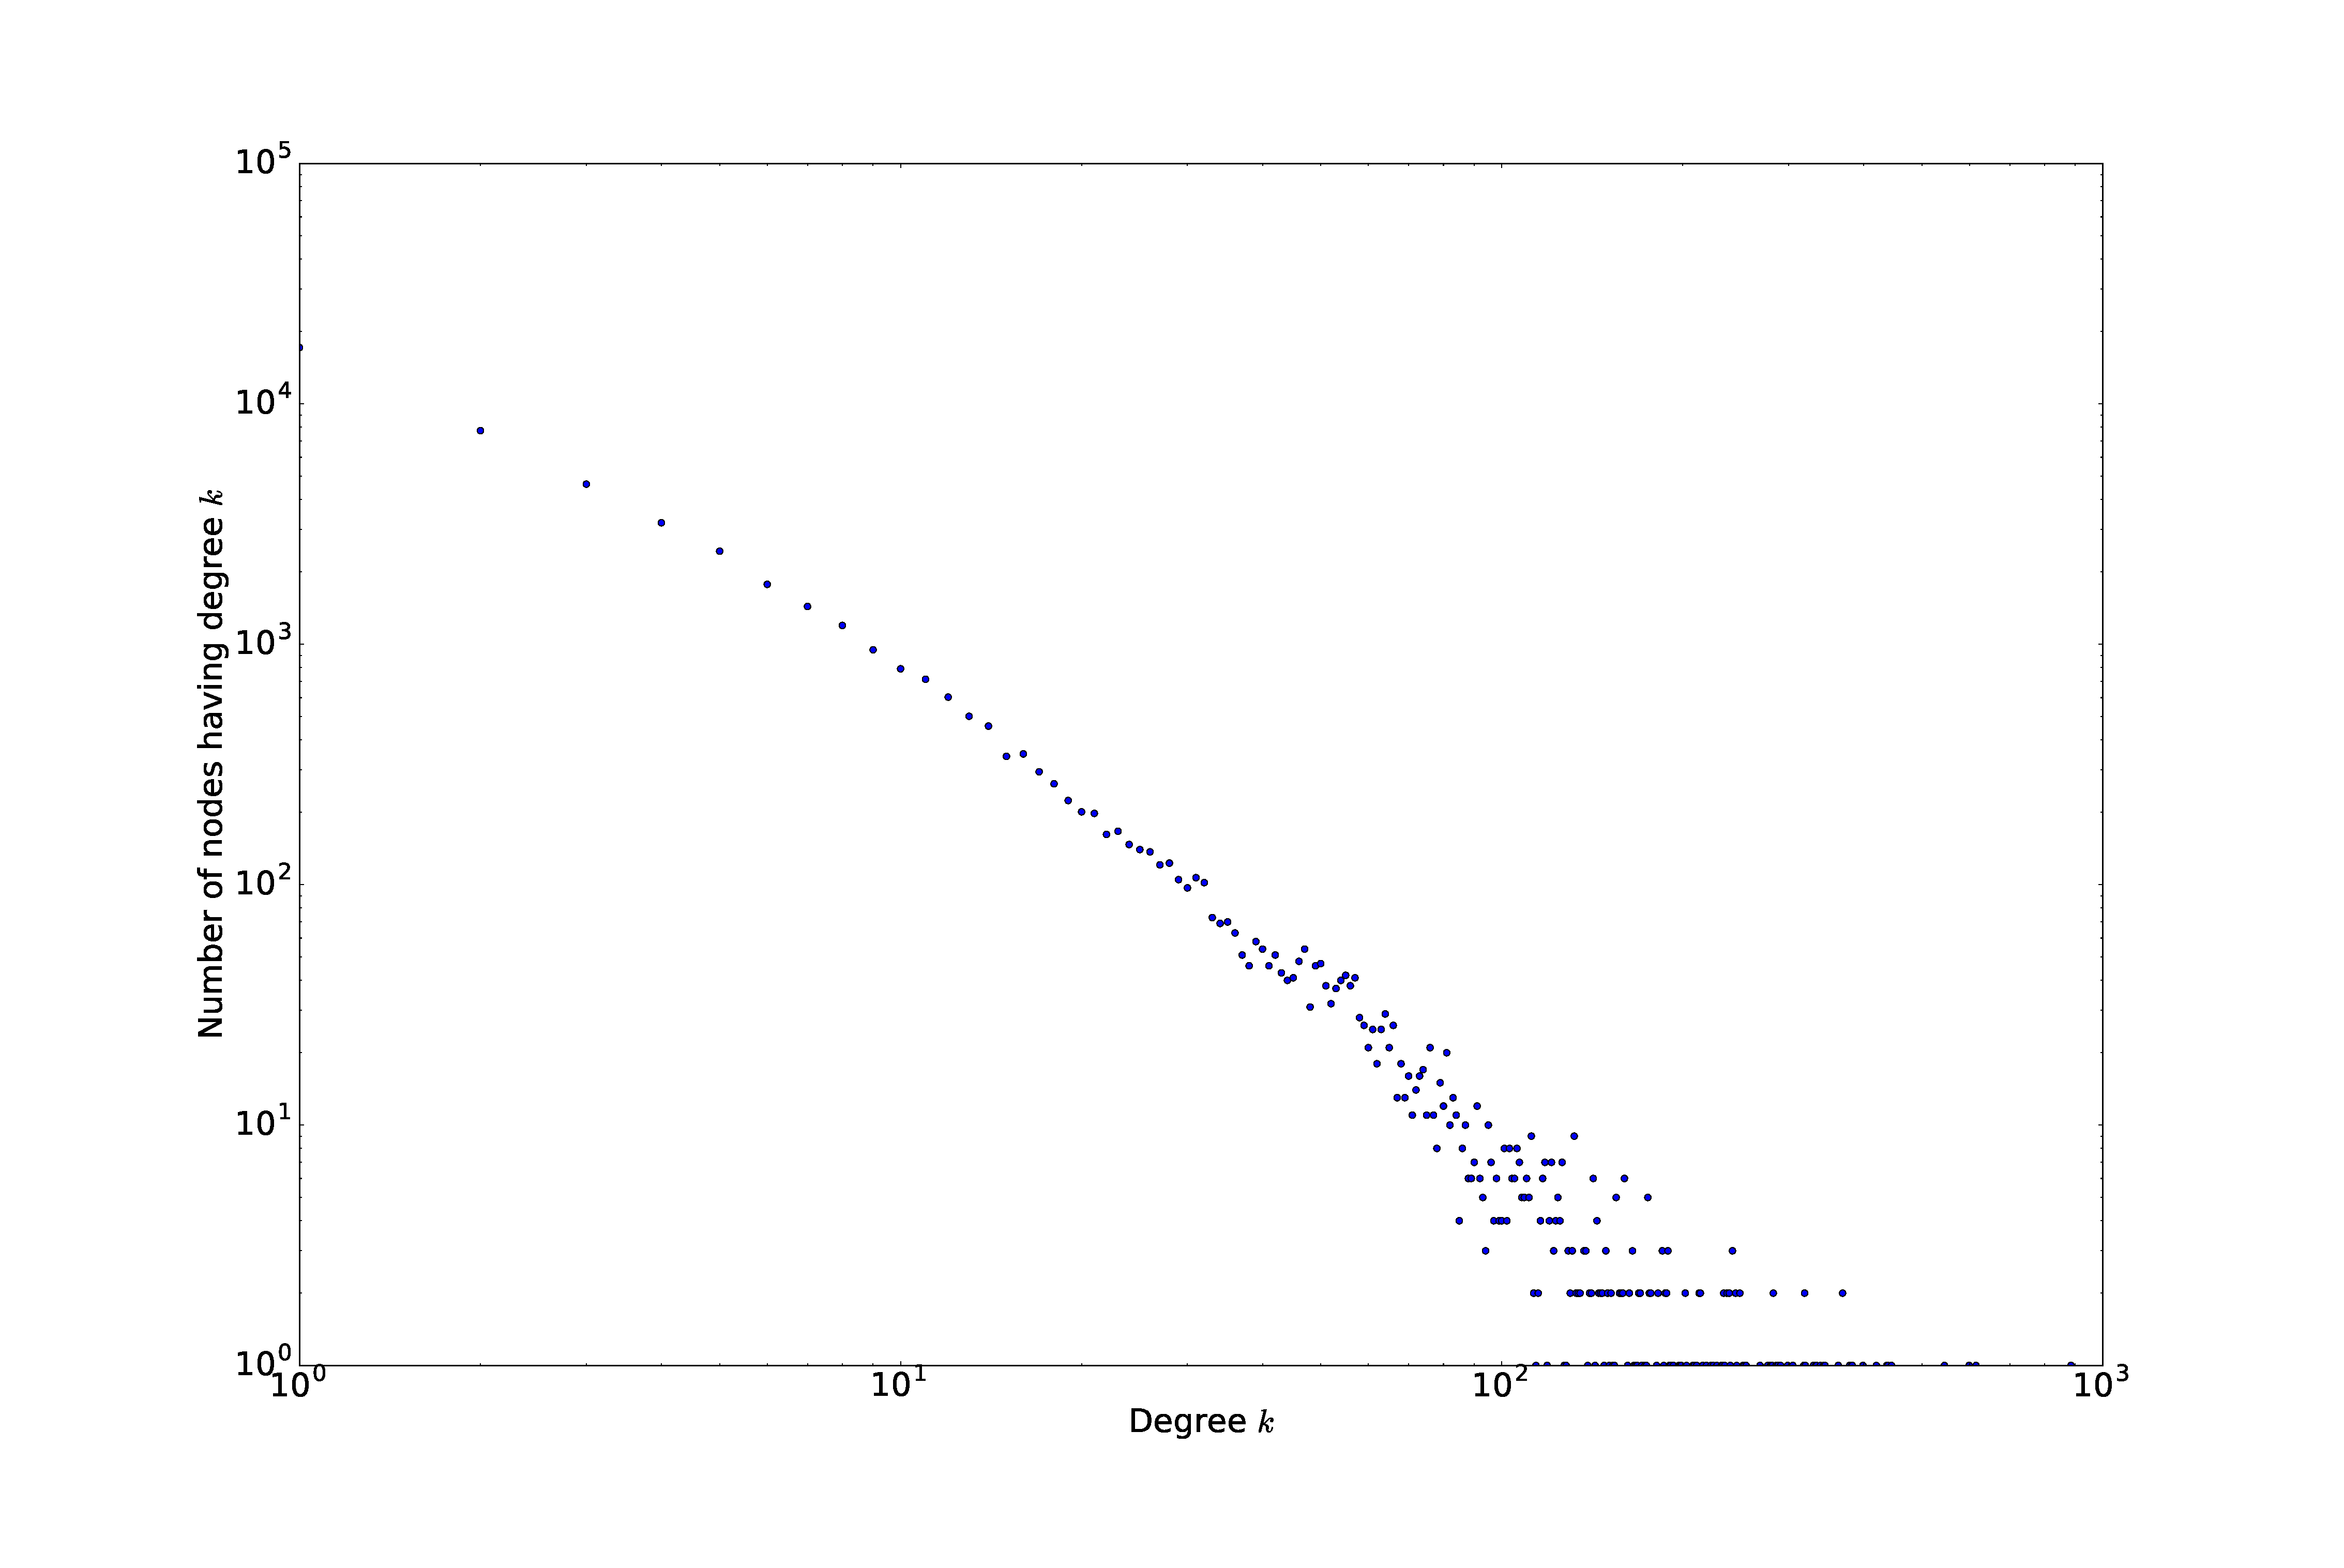
\includegraphics[width=100mm]{../fig/wot_degree_distribution.eps}}
     \caption{Web of Trustネットワークの次数分布}
     \label{fig:wot_dd}
    \end{figure}

  \acrshort{wot} $G$の解析の結果得られた基本情報を表\ref{table:wot_info}に示す. なお平均最短経路長はDijkstra法により, スケーリング指数については最小二乗法により求めた. 表\ref{table:wot_info}と\acrshort{wot}の次数分布をプロットした図\ref{fig:wot_dd}に見られるように, 高いクラスタリング係数, 小さな平均最短経路長, べき則に従う次数分布等, 典型的なスモールワールドネットワークかつスケールフリーネットワークの特徴が確認できる. 

 WoTをシミュレーション用実データとして用いている\cite{sandberg2006distributed}や\cite{clarke2010private}では以上に述べたのと同様の前処理の後さらにネットワークの局所的な部分グラフを取り出したり, 低次数ノードを削除するなどの操作を加えた後シミュレーションを行っているが, 本研究では現実のF2Fネットワークトポロジーにおけるルーティングのパフォーマンスをより正確に評価するために, まずはそういった意図的な操作は施さずにシミュレーションを行う. 以下では無向グラフとみなせる部分グラフを抽出する最低限の前処理が施されたのみで, 意図的な操作が加えられていないデータを便宜的に「未処理のネットワーク」と呼ぶこととする.

未処理のネットワークに対するシミュレーション後, ハブノードの消失に対する頑健性を考察するために次数上限を設けたネットワークに対するシミュレーションを行った. 以下$k_{\max}$を次数上限とする. 2017年1月20日現在, FreenetのF2Fモードでは特に接続ノード数の上限はないが, Opennetモードの接続数上限が100であるため, 本研究でも$k_{\max}=100$を基準とし, さらに$k_{\max}$を減少させた場合についても検証を行った. 実際にデプロイされたF2Fオーバーレイネットワークにおけるノードは個人利用のマシンが大半であると想定されるため, 100という数字は同時接続数制限として妥当な数字と考えられる. また, 実際今回用いたWoTネットワークにおいて次数が100を超えるノードは全ノードの1\%にも満たないため, 耐障害性の観点から, これら少数のハブノードの消失がルーティングパフォーマンスに及ぼす影響を評価することは非常に重要である.

なお今回行ったシミュレーションに関わる全てのソースコードはGitHubレポジトリ(\url{https://github.com/akiratk0355/navigable-network-analysis})にて誰もが閲覧可能である.


  \subsection{シミュレーション結果}
   \subsubsection{未処理のネットワークに対する結果}
   まずWoTネットワークをID空間に埋め込んだ様子を図\ref{fig:wot_emb}に示す. (a)の図は各ノードに独立にランダムなIDを割り当てただけのもので, (b)は(a)を初期状態としてSWAPアルゴリズムを適用し$6000|V|$回反復した後の様子を表す. Kleinbergモデルによって生成されたグラフの配置と同様に(b)の図には「距離が近いノードどうしほどエッジを持ちやすい」という特徴が現れており, Kleinbergモデルの性質が「復元」されたのが視覚的にも確認出来る. \newline
   またlocal contactの存在率$p_{\rm{local}}$を以下のように定義する.
   \begin{eqnarray*}
    p_{\rm{local}} = \frac{\mbox{ID空間上で最も近距離にいるノード同士を接続するエッジの本数}}{|V|}
   \end{eqnarray*}
   $p_{\rm{local}}$を(a), (b)について共に算出したところ, (b)の方がlocal contactの存在率が高くなっているものの1.0からは程遠いため, 埋め込み後のネットワークにおける単純なgreedyルーティングの効率性が担保されないことが, この時点ですでに予測される.

   \begin{figure}[htbp]
    \centering
    \begin{subfigure}[b]{0.48\textwidth}
        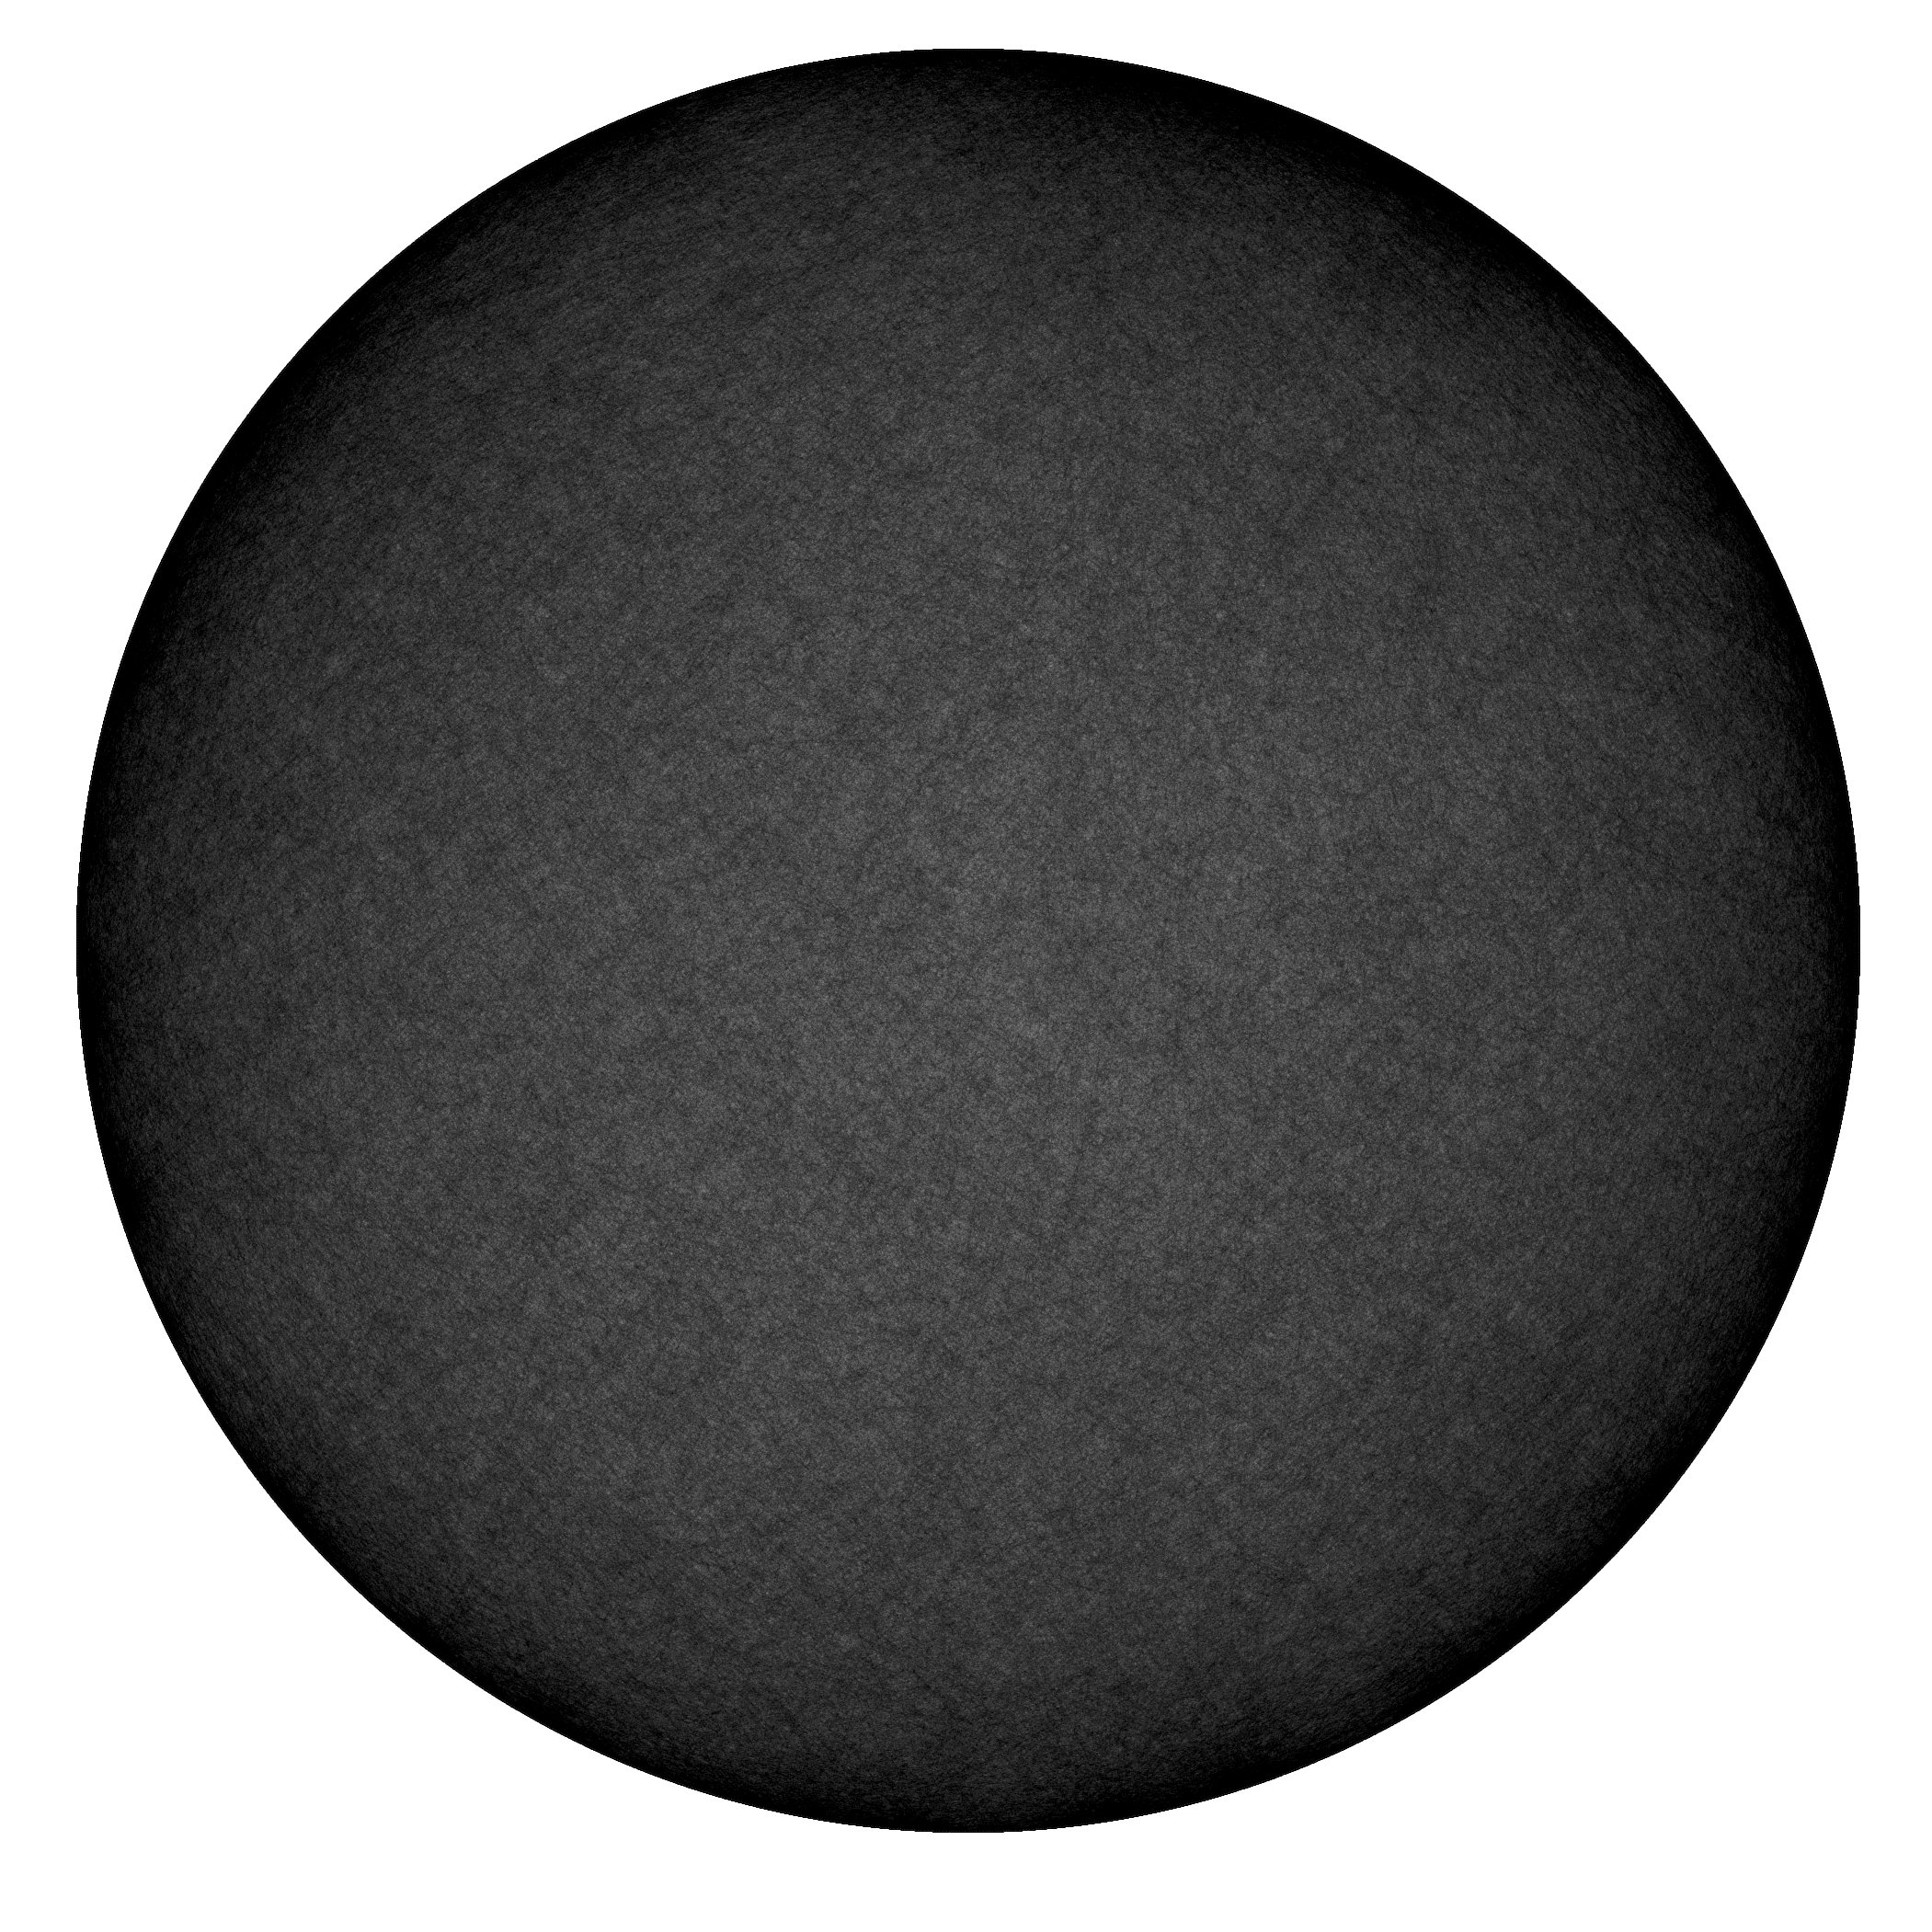
\includegraphics[width=\textwidth]{../fig/wot_default_random_thesis.png}
        \caption{SWAP適用前 \\ $p_{\rm{local}} = 0.0002$}
    \end{subfigure}
    \begin{subfigure}[b]{0.48\textwidth}
        \includegraphics[width=\textwidth]{../fig/wot_emb_sandberg_thesis.png}
        \caption{SWAP適用後 \\ $p_{\rm{local}} = 0.23$}
    \end{subfigure}
    \caption{ID空間$C=[0,1)$に埋め込まれたWeb of Trustネットワーク}
    \label{fig:wot_emb}
   \end{figure}

   次に図\ref{fig:wot_emb}(b)のネットワークに対するルーティングシミュレーションを行った結果を図\ref{fig:succ_hops_full}, \ref{fig:cml_noclip}に示す.  シミュレーションの結果$D^3$-$DFS$は$D^2$-$DFS$を15\%以上成功率で上回り, にも関わらず平均ホップ数を20以上短縮するという大幅なパフォーマンスの改善を見せた. またEVNRと$D^3$-$DFS$は成功率, 平均ホップ数共に拮抗しており, 図\ref{fig:cml_noclip}から読み取れる通り, 各ホップ数内に成功したルーティングの割合は$D^3$-$DFS$がごく僅かに上回る結果となった. \cite{simsek2008navigating}では, 隣接ノードが全て訪問済みの場合ランダムに選ばれた隣接ノードにフォワードすることが最も高いパフォーマンスを記録したと述べられているが, 今回の実験結果はそれに反することがわかった.

   一方, 隣接ノードが全て訪問済みの場合にルーティング失敗とする3つのルーティングについて着目すると, 単純なgreedyルーティングのヒューリスティックを利用するFAILとCONTの成功率は非常に低いが, EVNのヒューリスティックを導入するだけで大幅な改善が見られた. これはたとえターゲットに近くとも次数が極端に低いノードにメッセージがフォワードがされづらくなったためと考えられる.

   \begin{figure}[htbp]
    \centerline{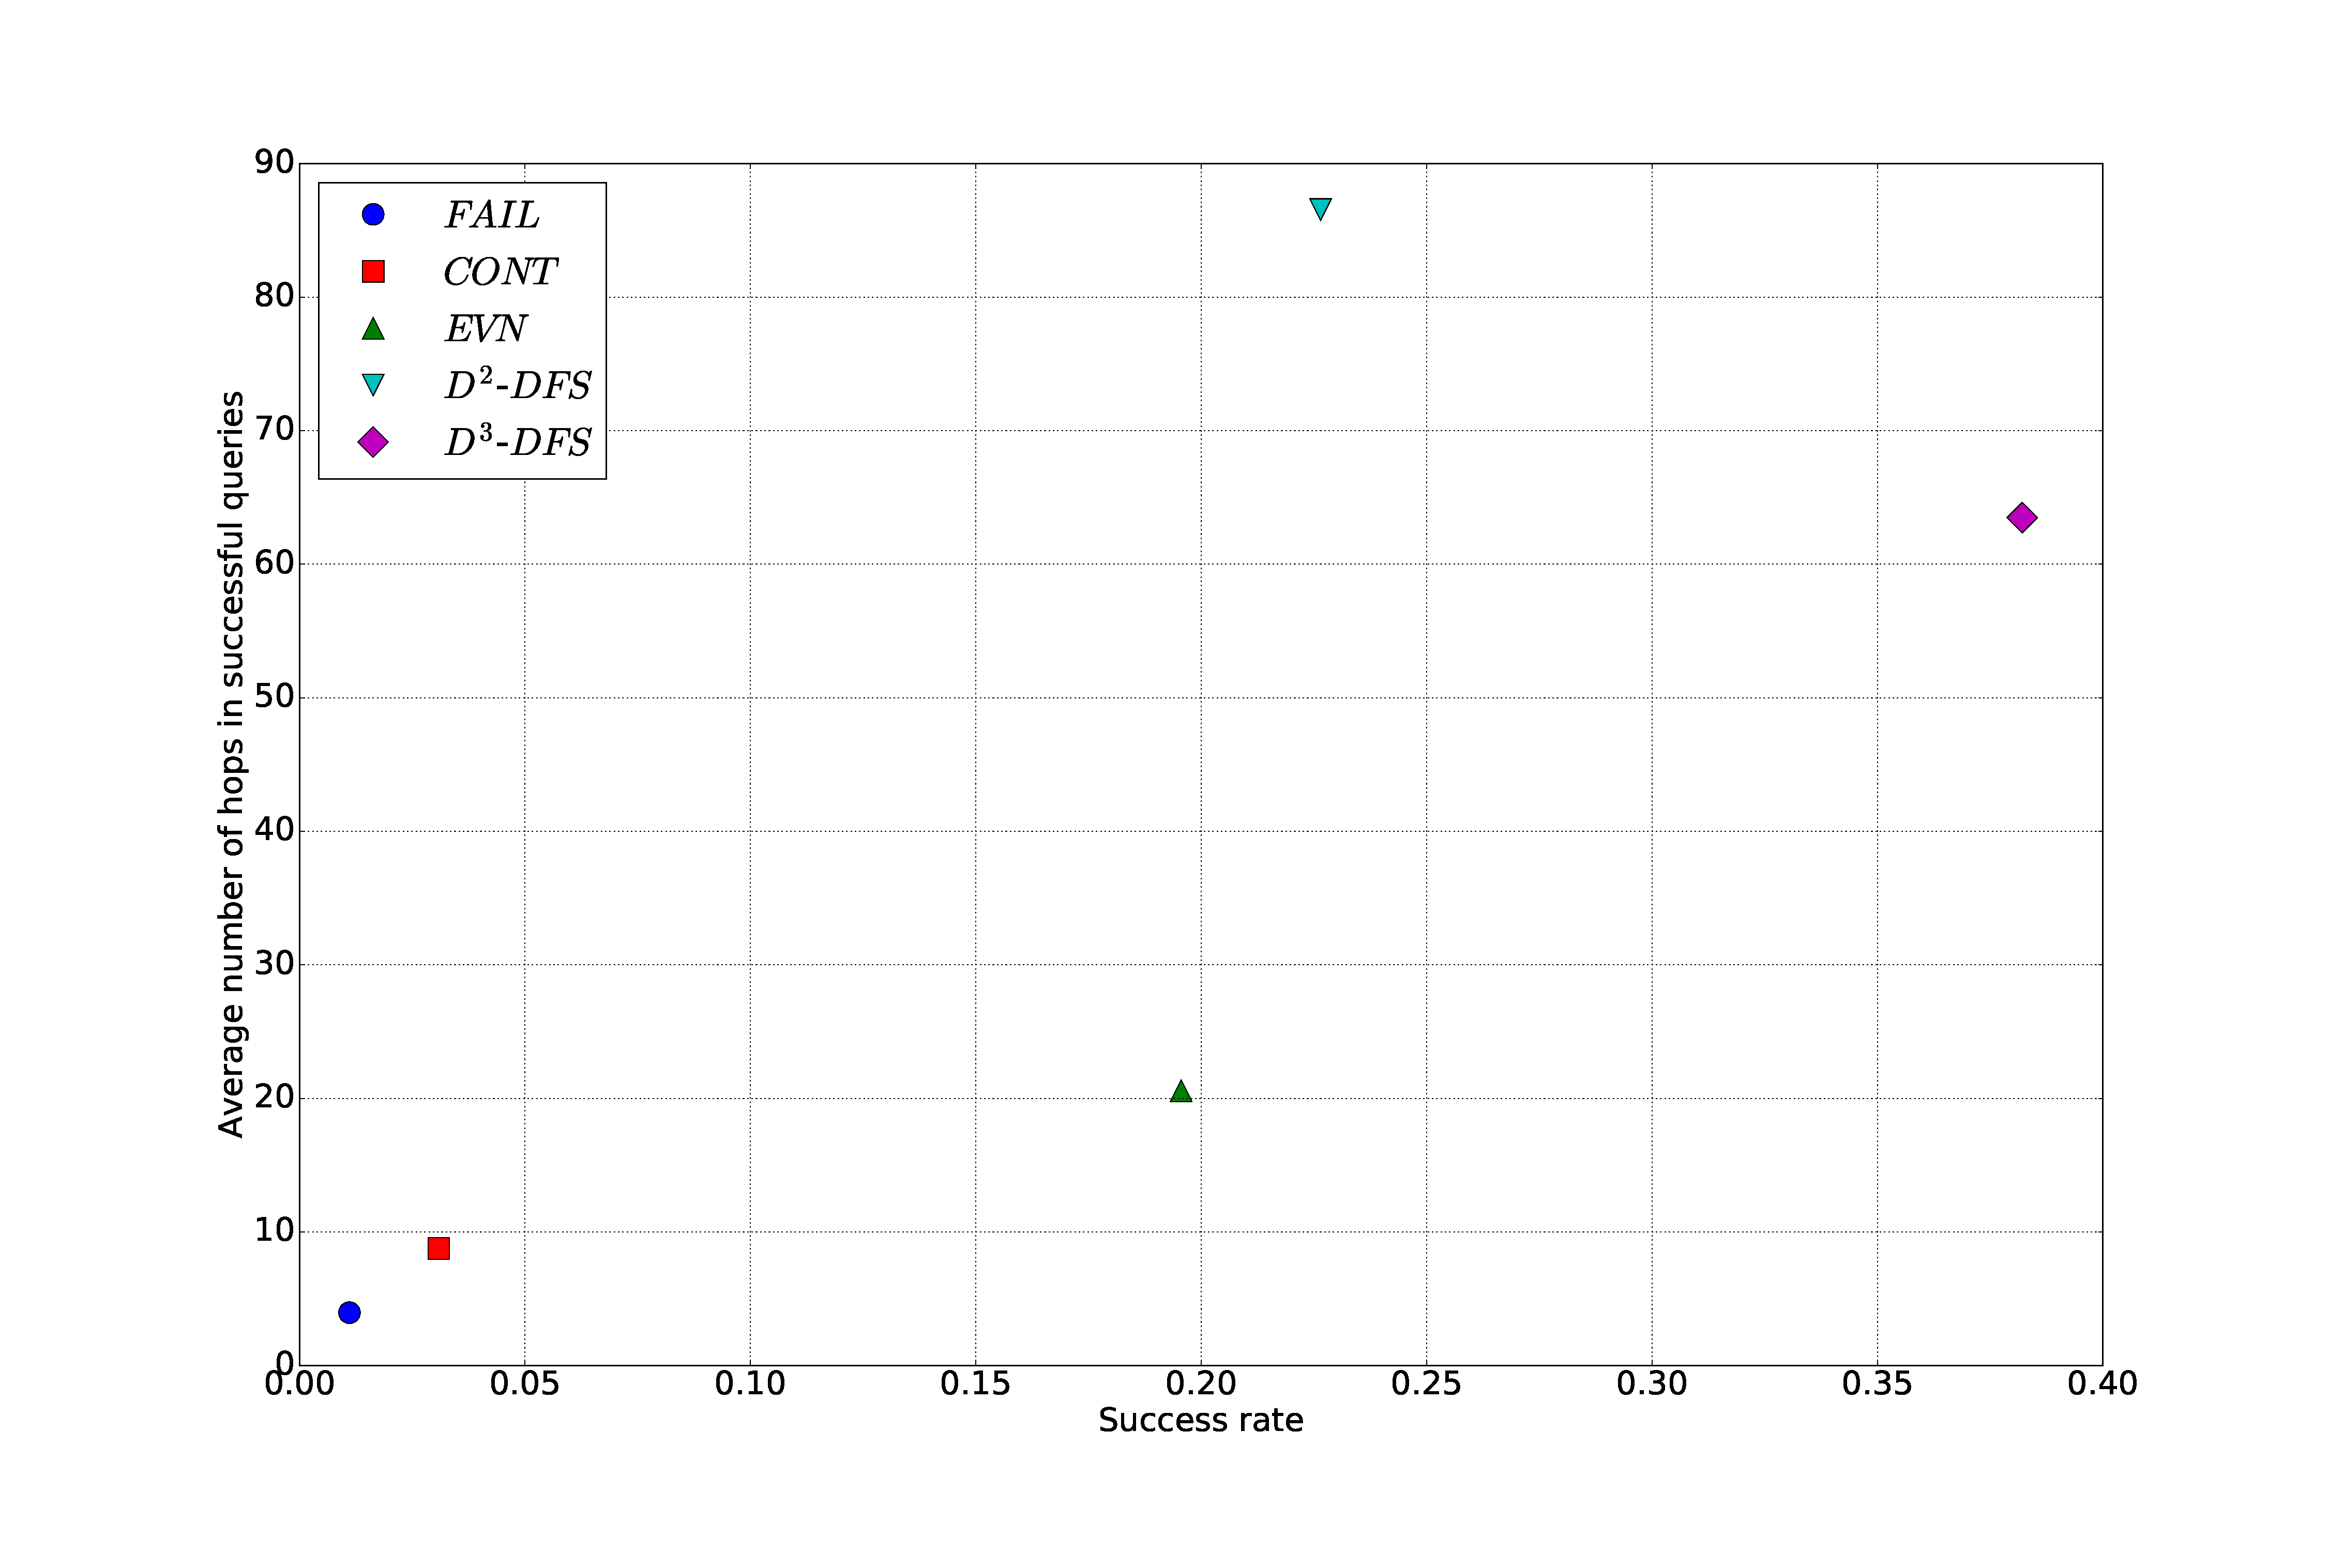
\includegraphics[width=100mm]{../fig/succ_hops_full.eps}}
    \caption{ID割り当て後のWeb of Trustネットワークにおける各ルーティングアルゴリズムの成功率と平均ホップ数}
    \label{fig:succ_hops_full}
   \end{figure}
   \begin{figure}[htbp]
    \centerline{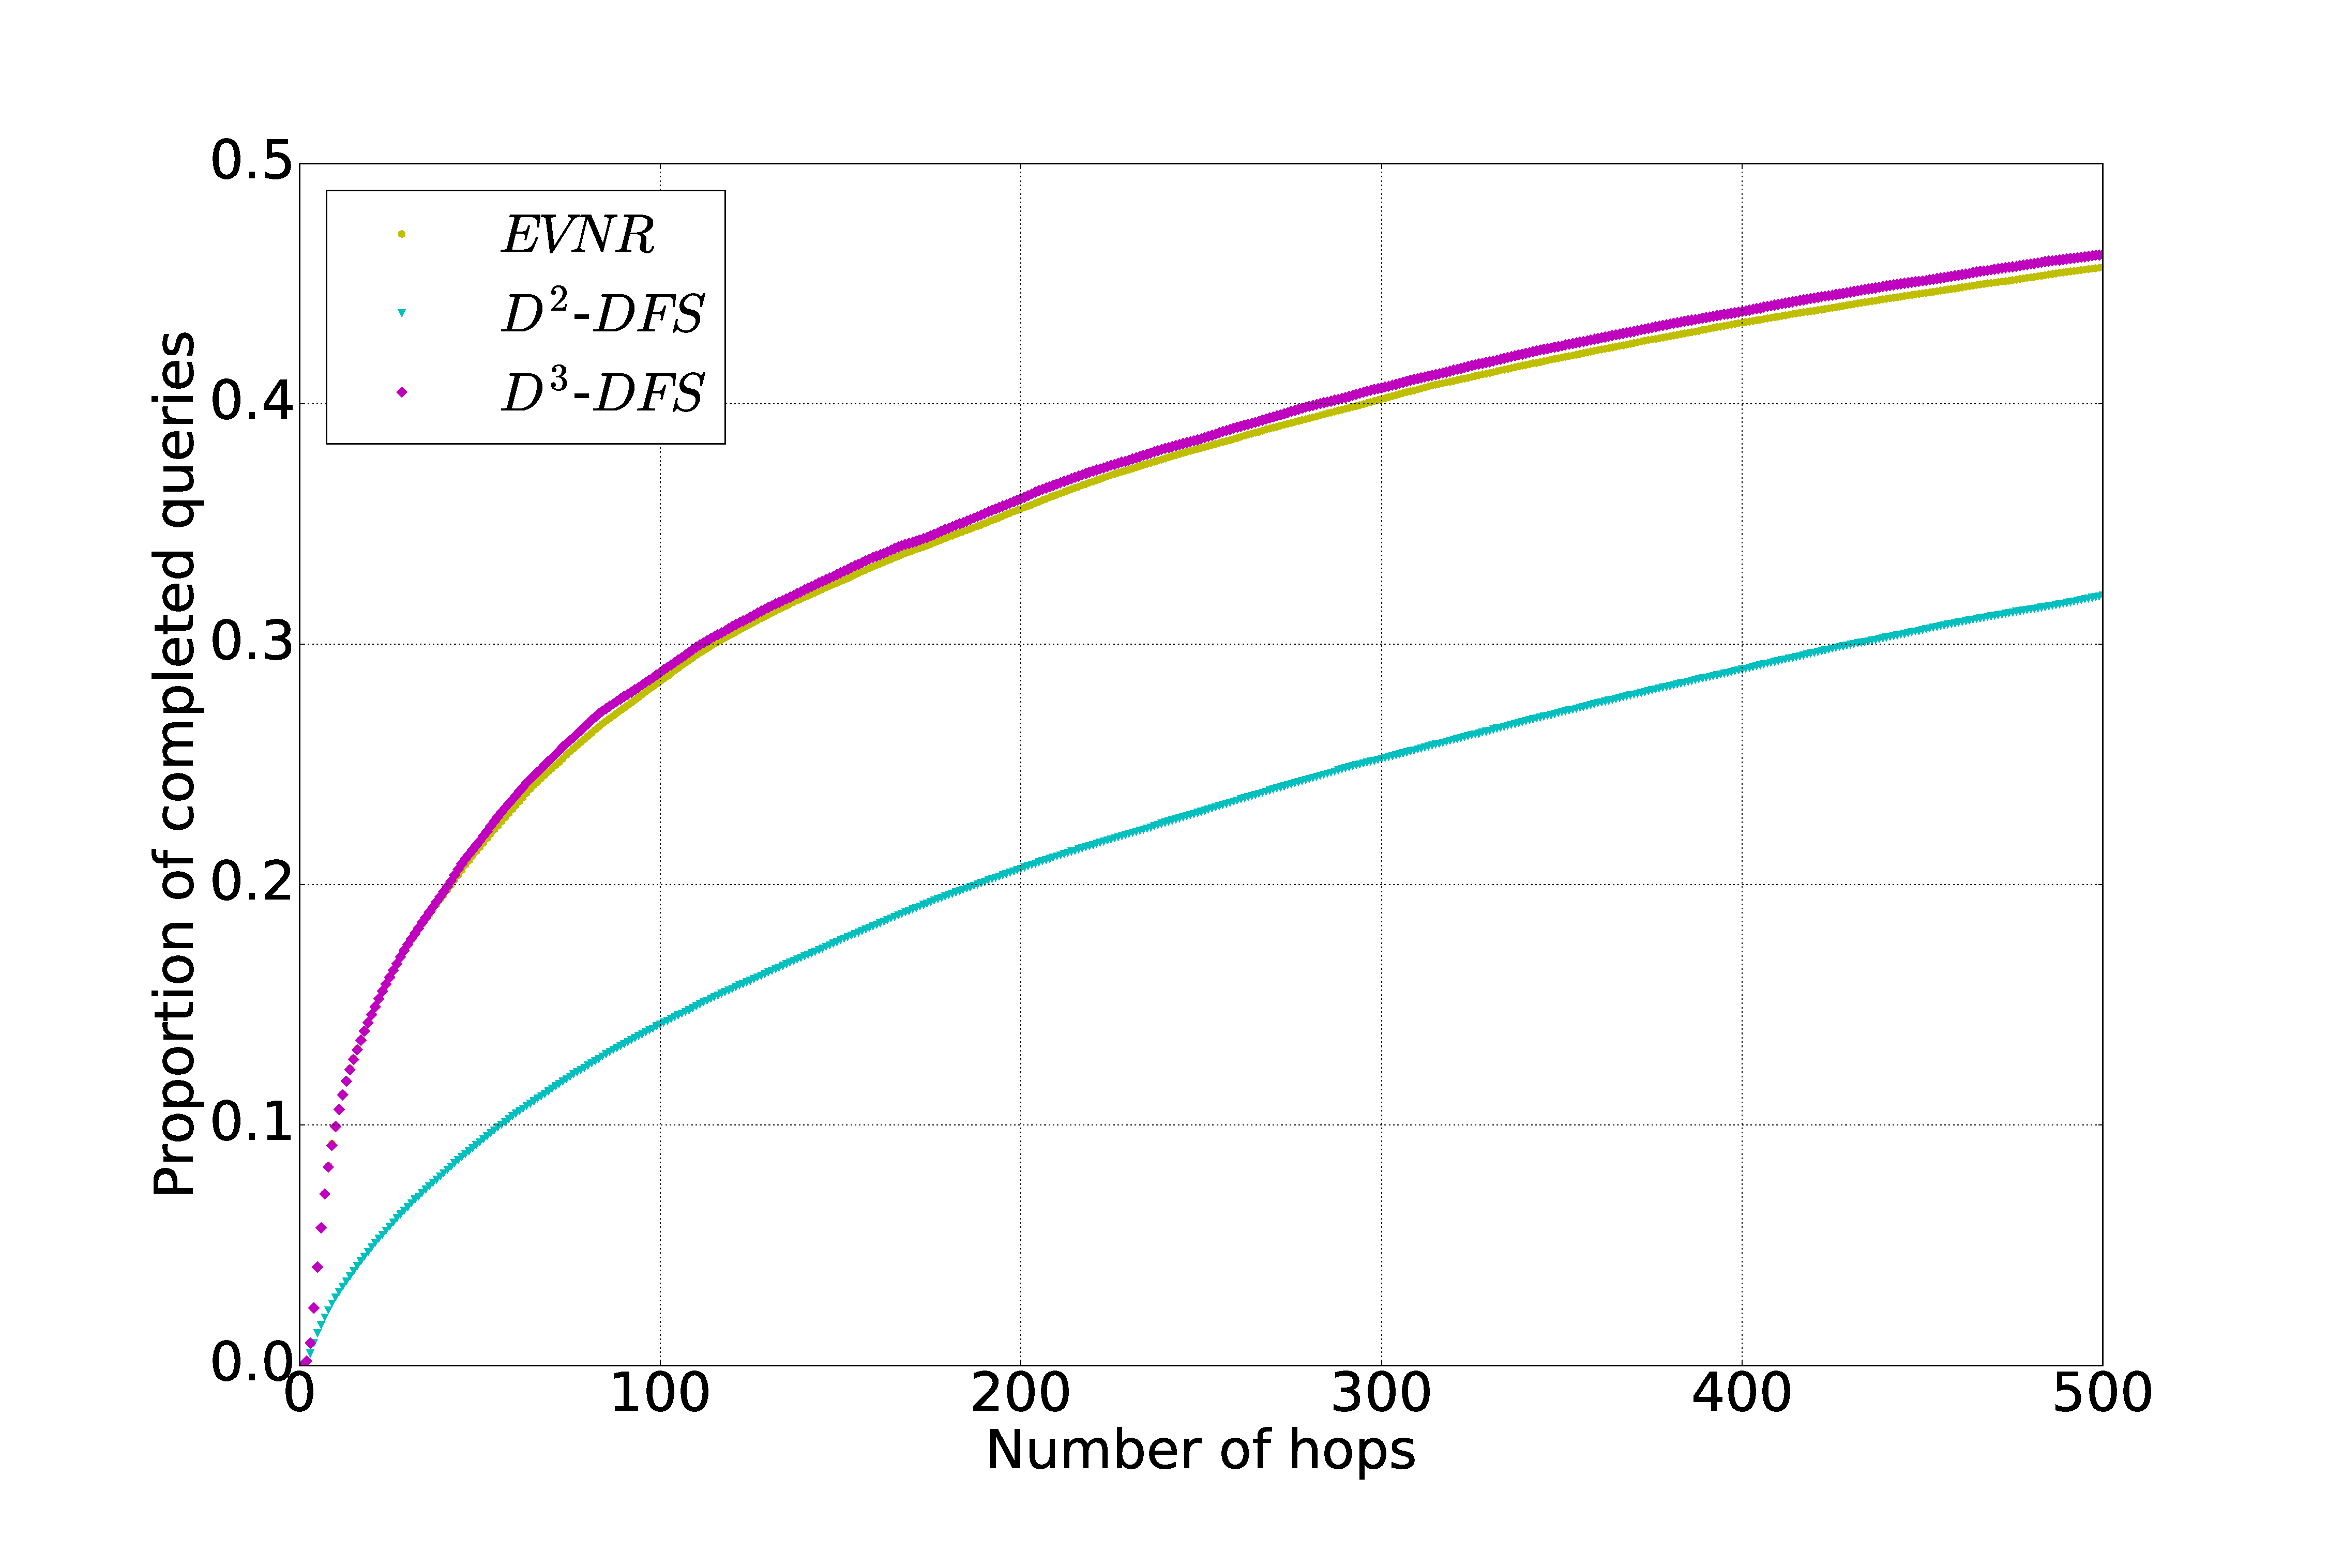
\includegraphics[width=100mm]{../fig/cml_noclip.eps}}
    \caption{ID割り当て後のWeb of Trustネットワークにおける各ホップ数以下で成功したルーティング試行の割合}
    \label{fig:cml_noclip}
   \end{figure}

   \subsubsection{次数上限を設けたネットワークに対する結果}
   未処理のWoTネットワークデータに次数上限を設け, ネットワーク全体でごく僅かな割合を占める少数のハブノードを取り除いた後のネットワークに対して前節と同じシミュレーションを埋め込みの段階も含めて行った際の結果を図\ref{fig:clip_succ}, \ref{fig:clip_hops}, \ref{fig:cml_dclip}に示す.

   概ねの傾向としていずれのルーティングアルゴリズムにおいても$k_{\max}$が減少するに応じて, 成功率が低下していることがわかった. つまりgreedyルーティングにせよ, EVNのヒューリスティックにせよ, 少数のハブの存在がルーティングのパフォーマンス向上に寄与していることになる. また, 次数上限がある中でも成功率や各ホップ数以内に成功したルーティング試行の割合の面でルーティングアルゴリズムの優劣は基本的に変わらず, $k_{\max}=10$の場合を除き, $D^3$-$DFS$, EVNR, $D^2$-$DFS$の順に高いパフォーマンスを発揮した.

   よって$D^3$-$DFS$はハブノードの存在によって恩恵を受けており, ハブの消失により確かに絶対的なパフォーマンスは低下するものの, 既存ルーティングアルゴリズムも同様にパフォーマンスが低下するため, 相対的には優れた性能を持ったアルゴリズムであることが分かる. これはEVNのヒューリスティックがgreedyルーティングのそれを包含しており, 次数のばらつきがない場合にEVNのヒューリスティックは単なる距離に基づいたものとなるからである.

   \begin{figure}[htbp]
    \centerline{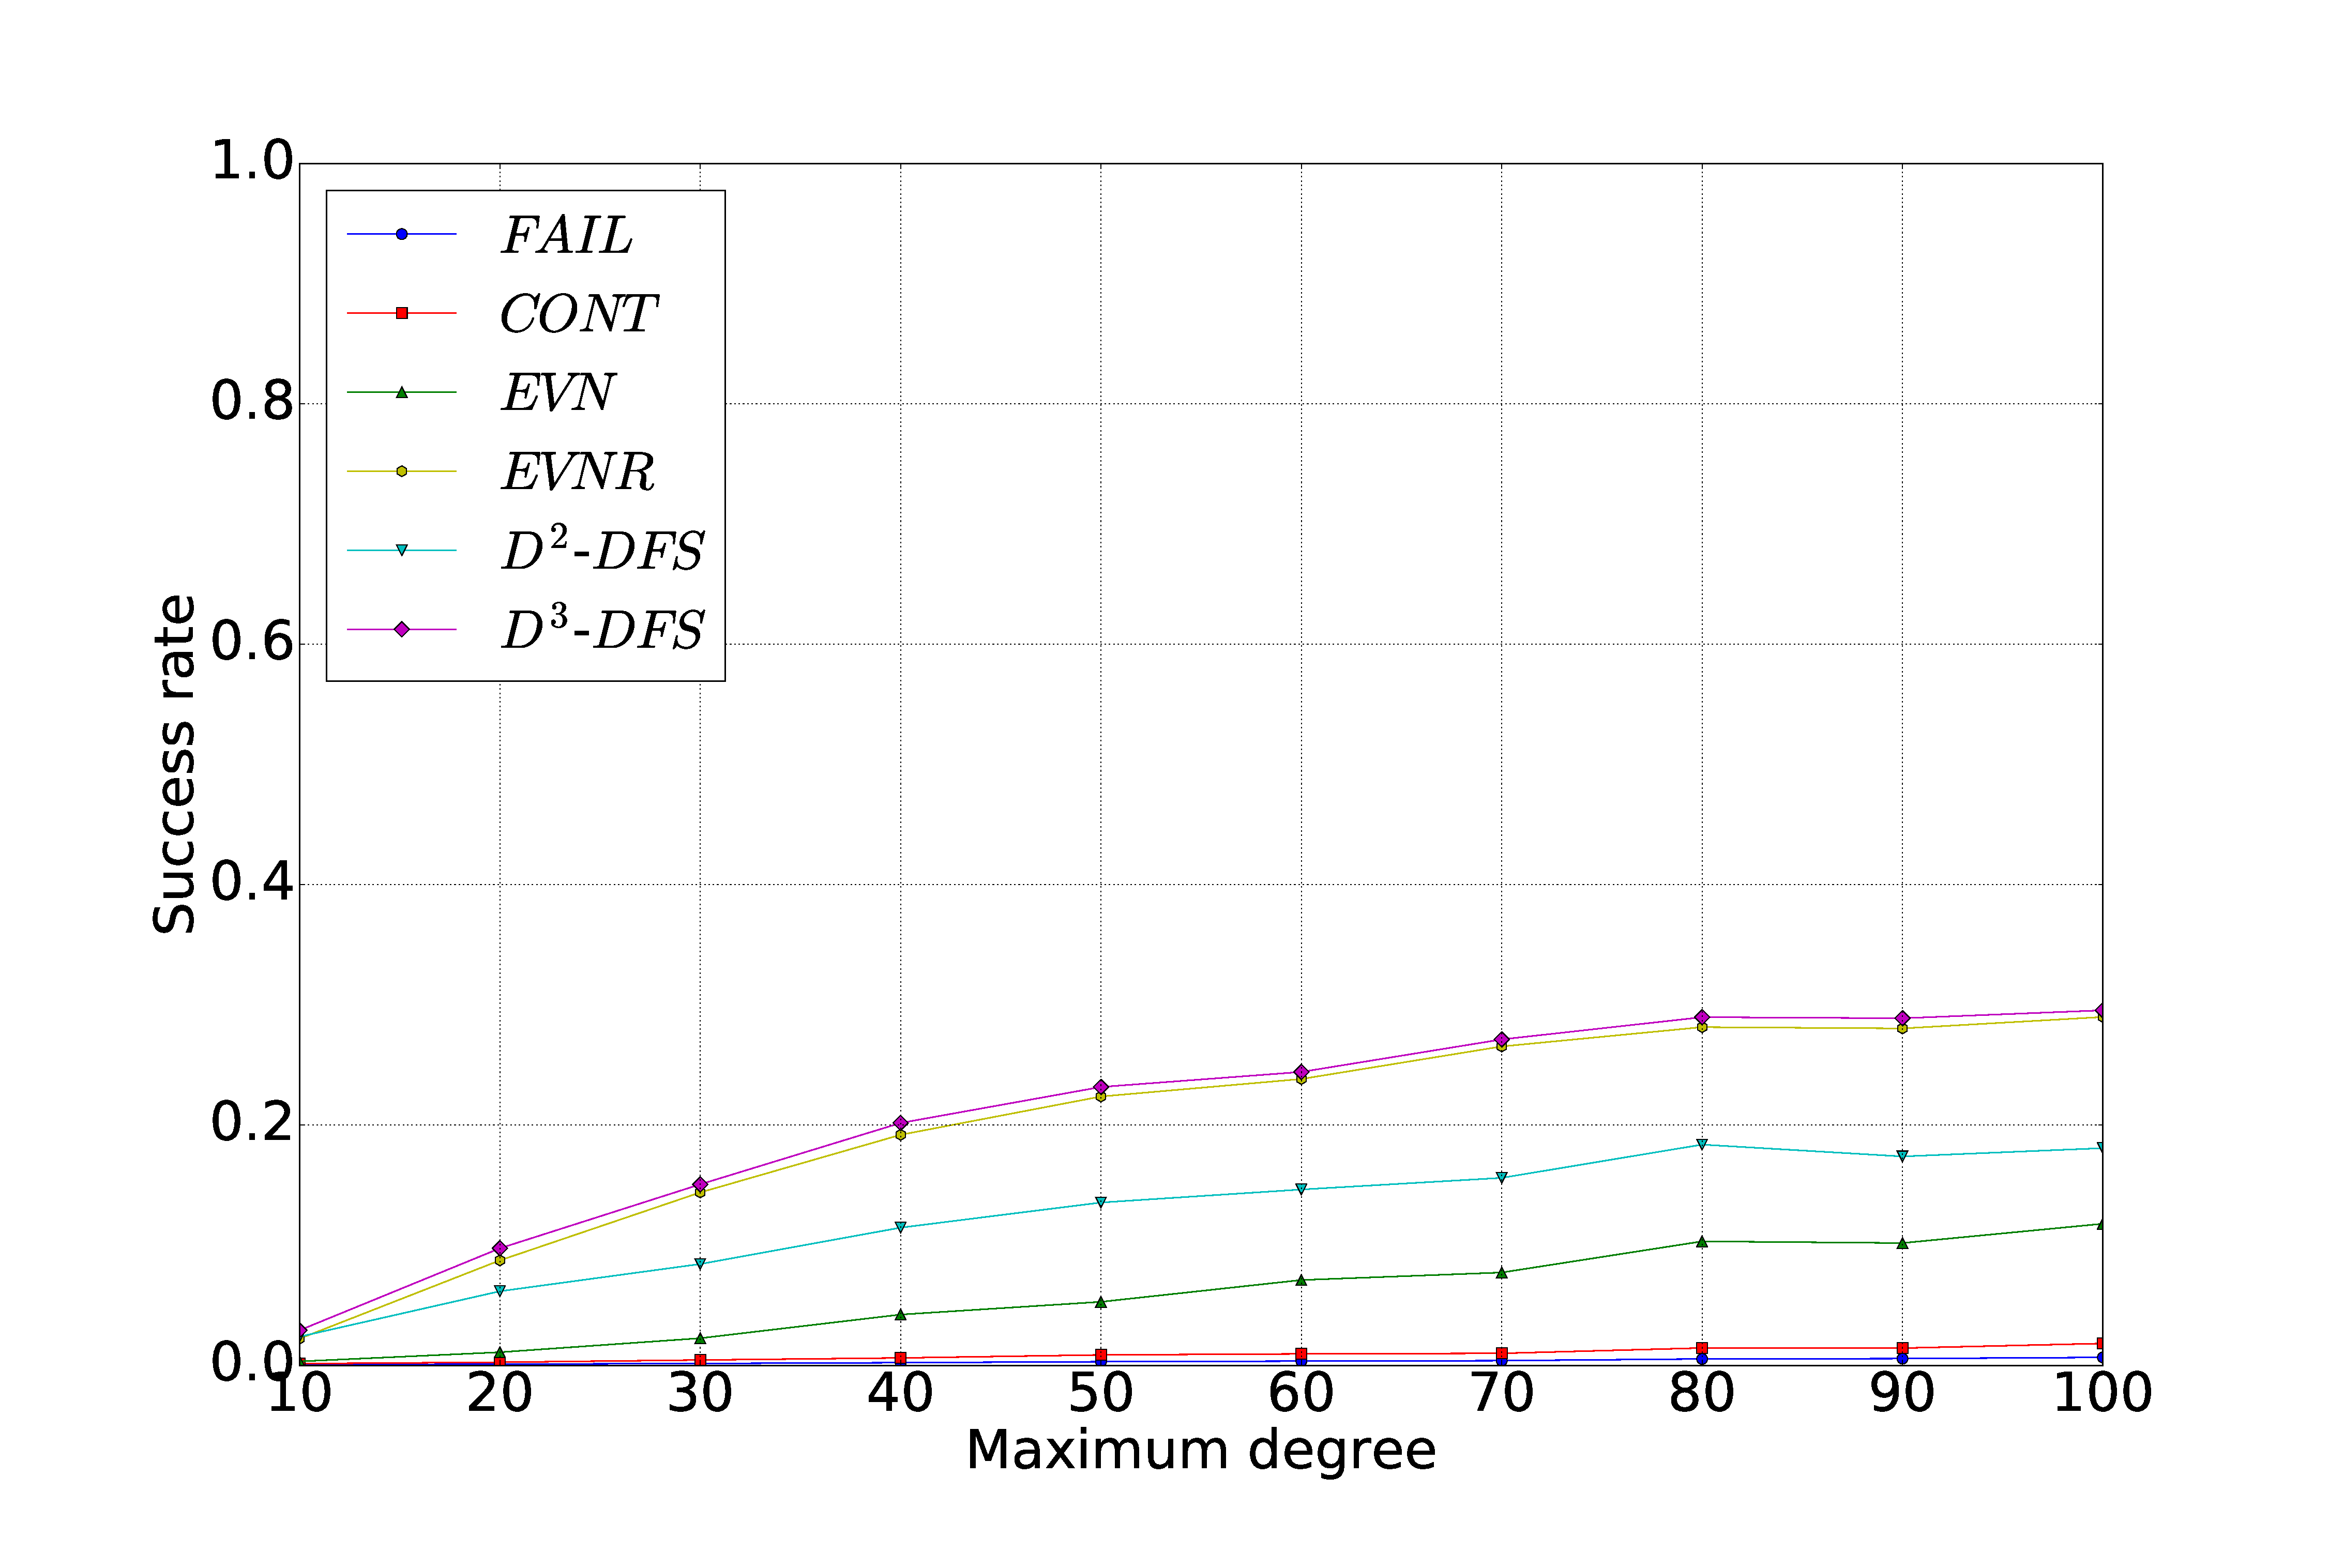
\includegraphics[width=100mm]{../fig/clip_succ.eps}}
    \caption{次数上限を設定したWeb of Trustネットワークにおける各ルーティングアルゴリズムの成功率}
    \label{fig:clip_succ}
   \end{figure}

   \begin{figure}[htbp]
    \centerline{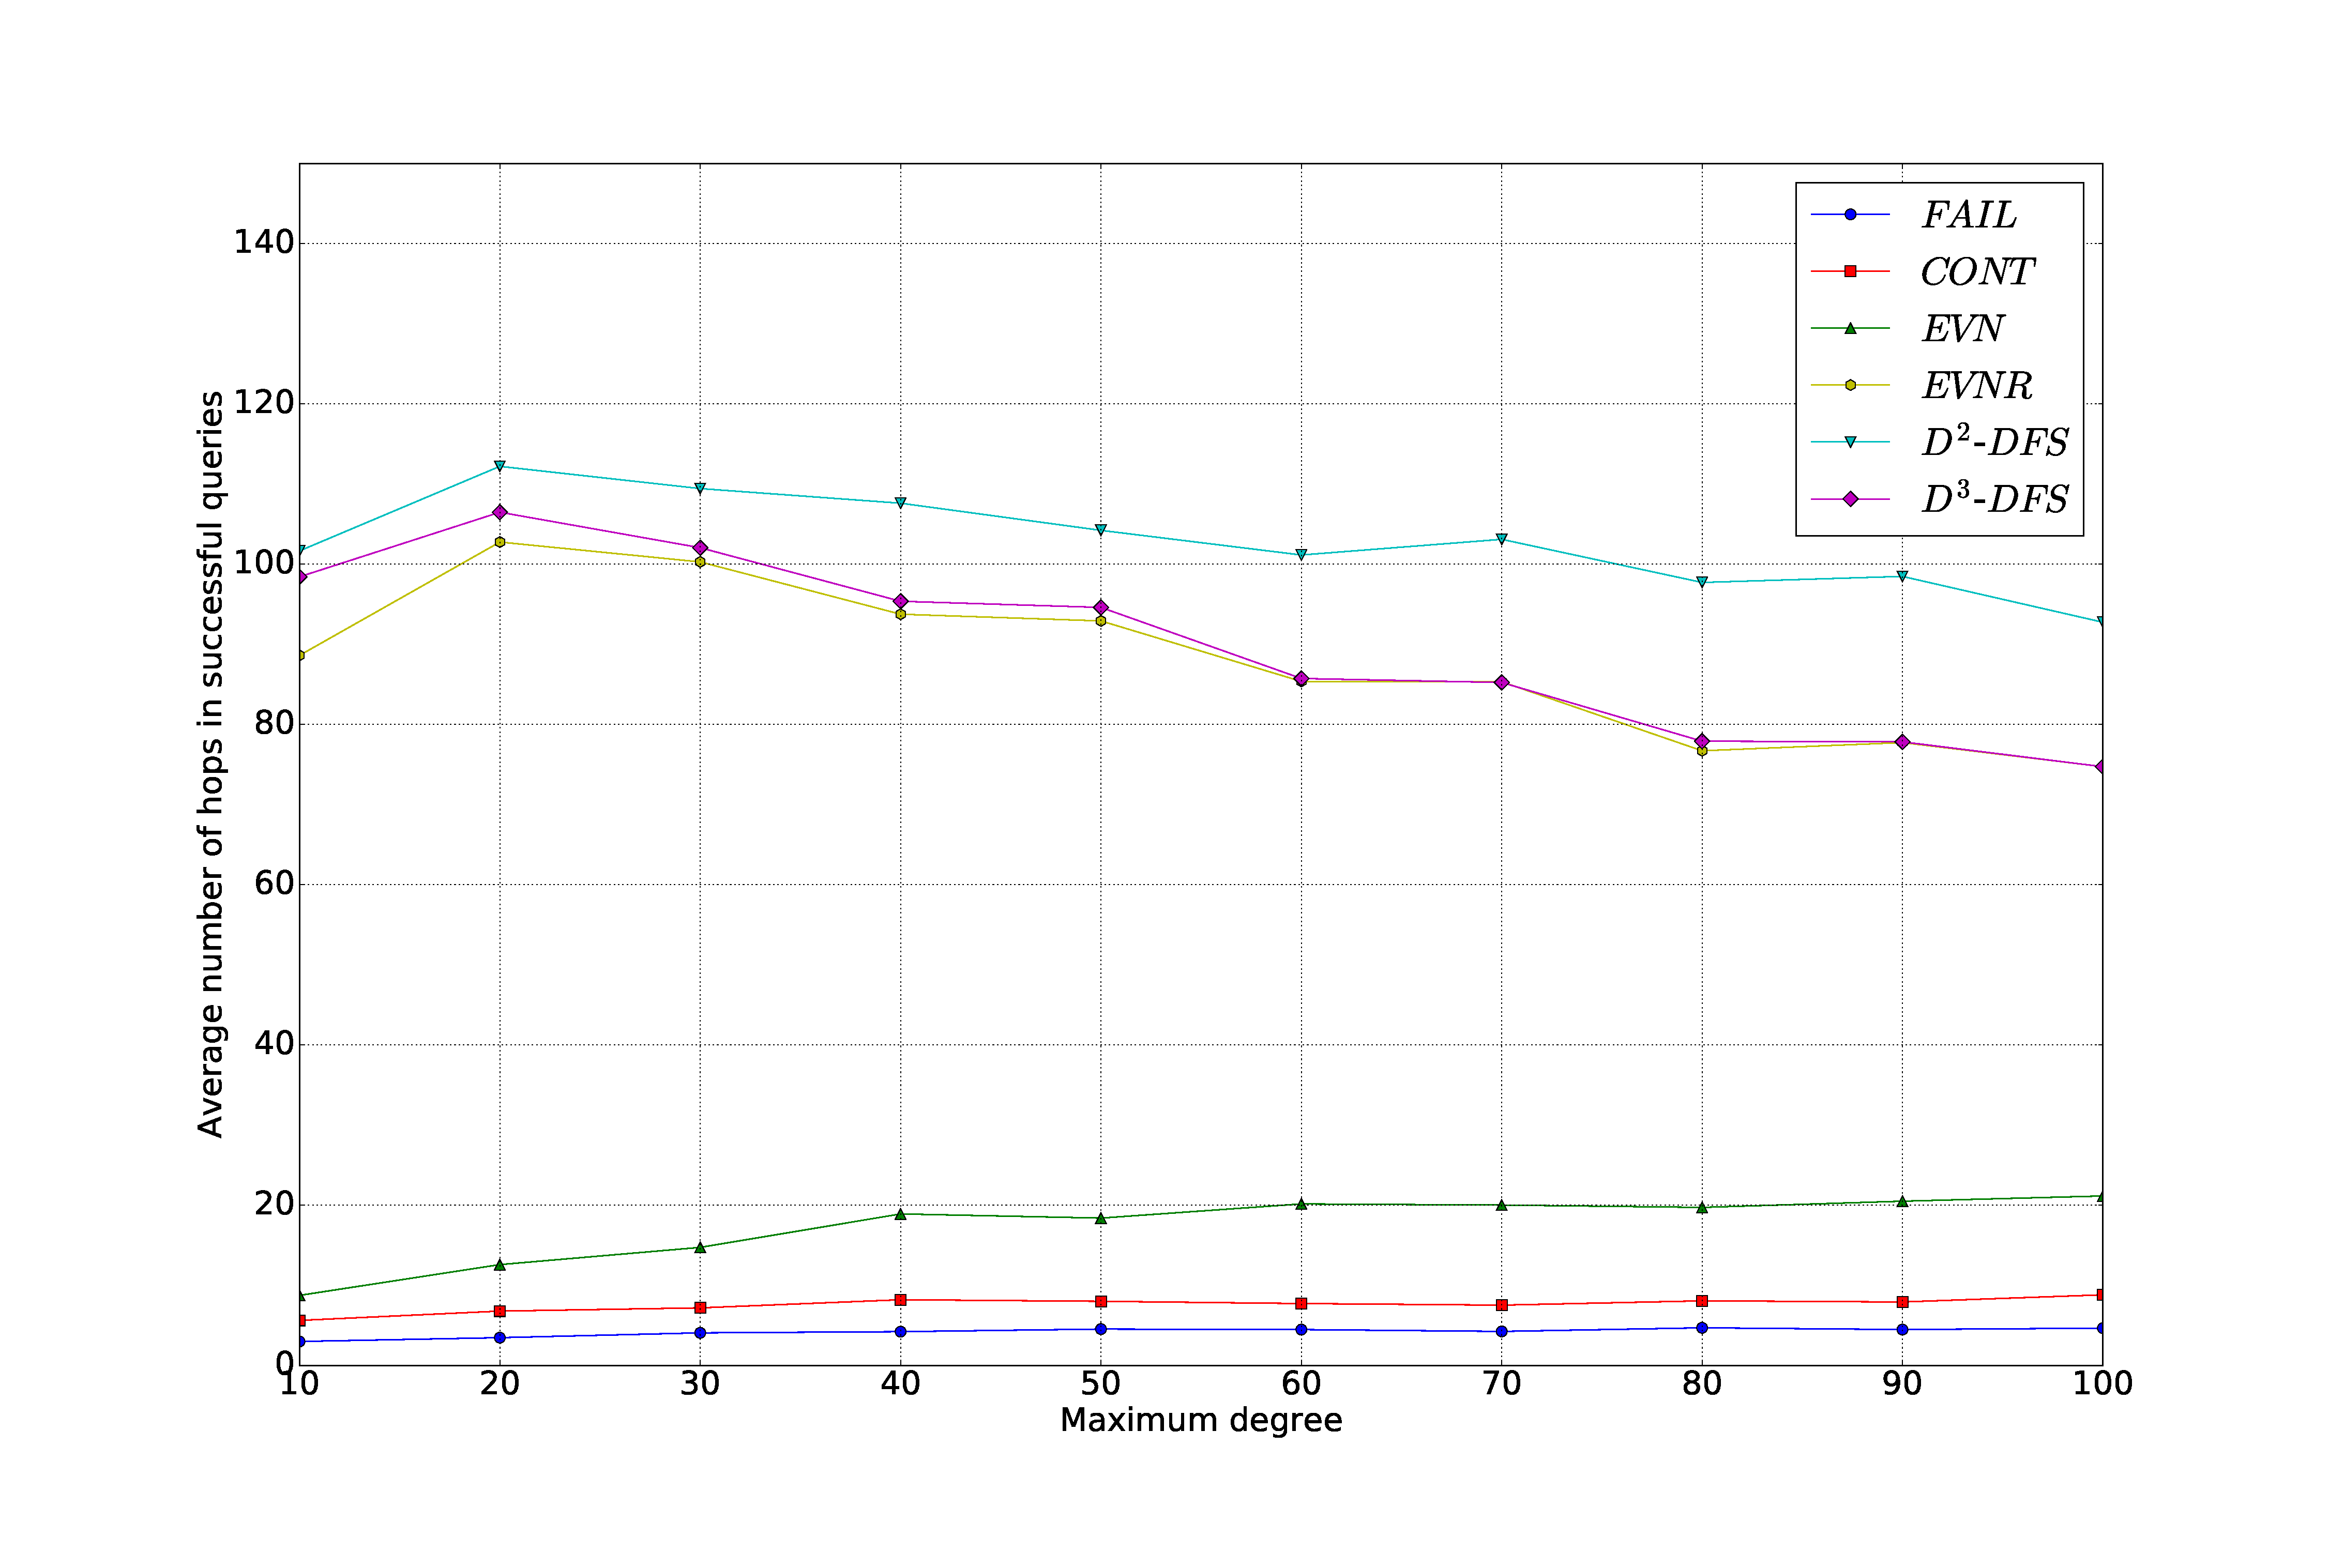
\includegraphics[width=100mm]{../fig/clip_hops.eps}}
    \caption{次数上限を設定したWeb of Trustネットワークにおける各ルーティングアルゴリズムの平均ホップ数}
    \label{fig:clip_hops}
   \end{figure}

   \begin{figure}[htbp]
    \begin{minipage}{0.33\hsize}
     \begin{center}
      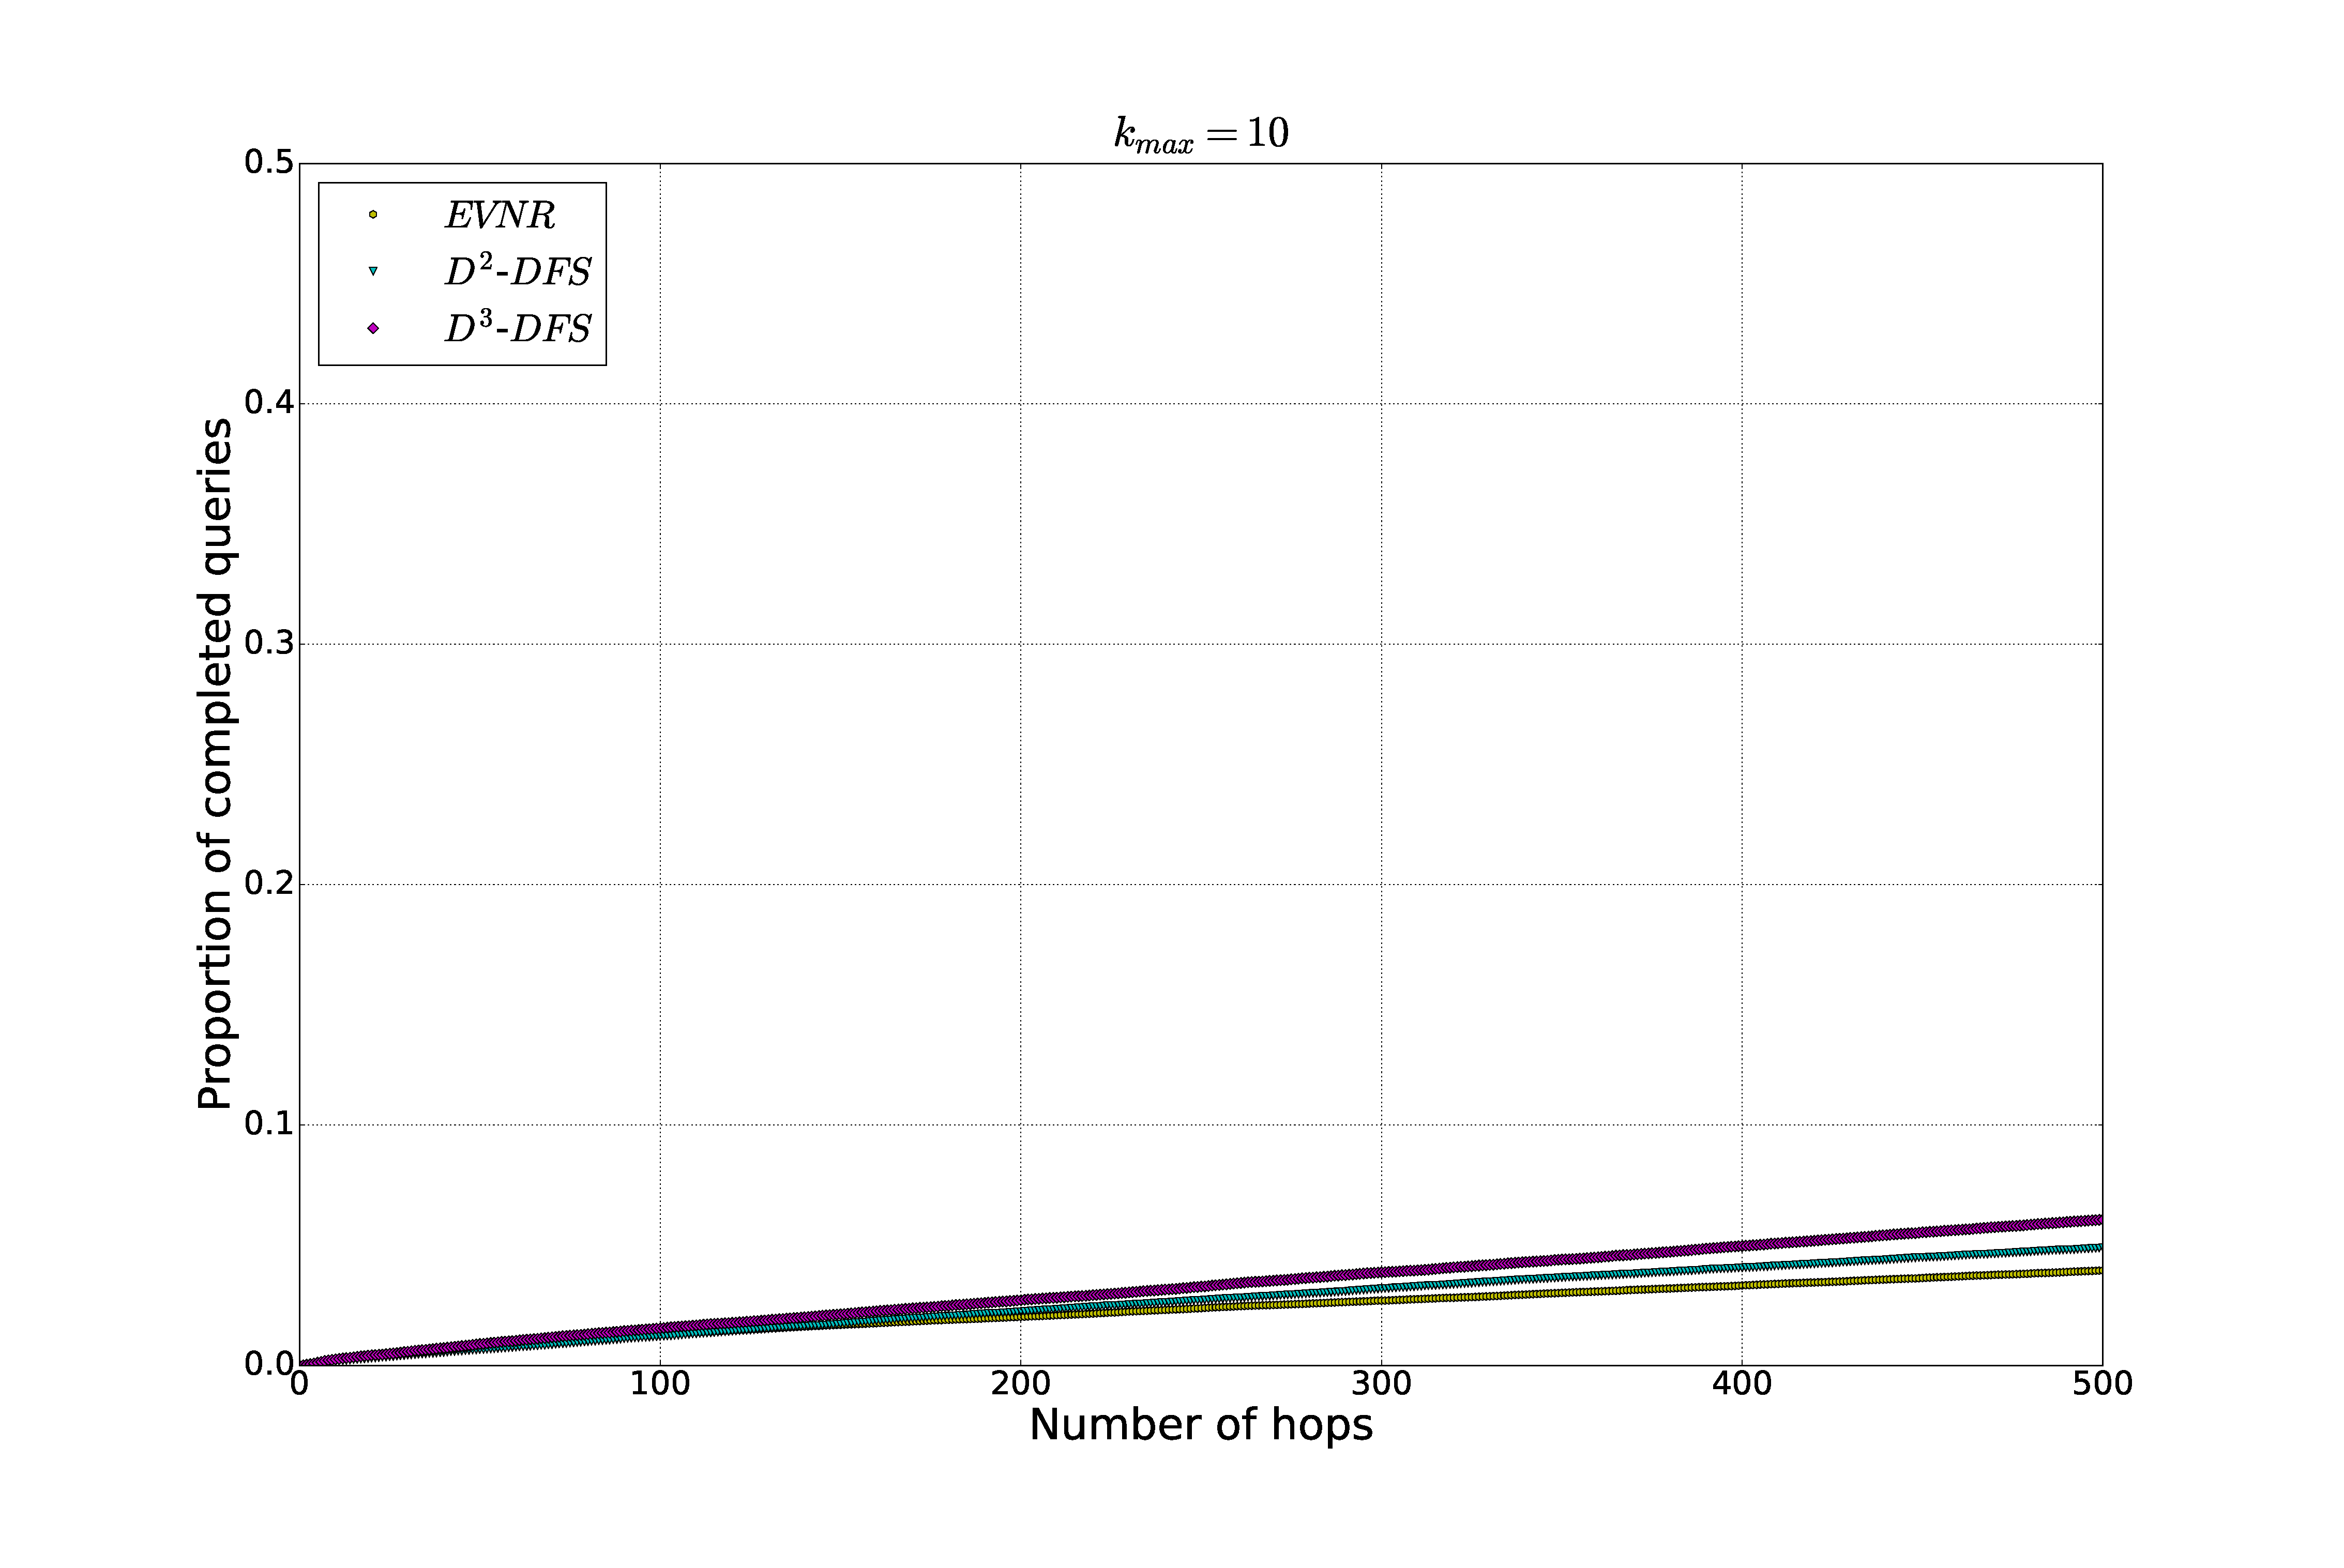
\includegraphics[width=47mm]{../fig/cml_10clip.eps}
     \end{center}
     \label{fig:11}
    \end{minipage}\begin{minipage}{0.33\hsize}
     \begin{center}
      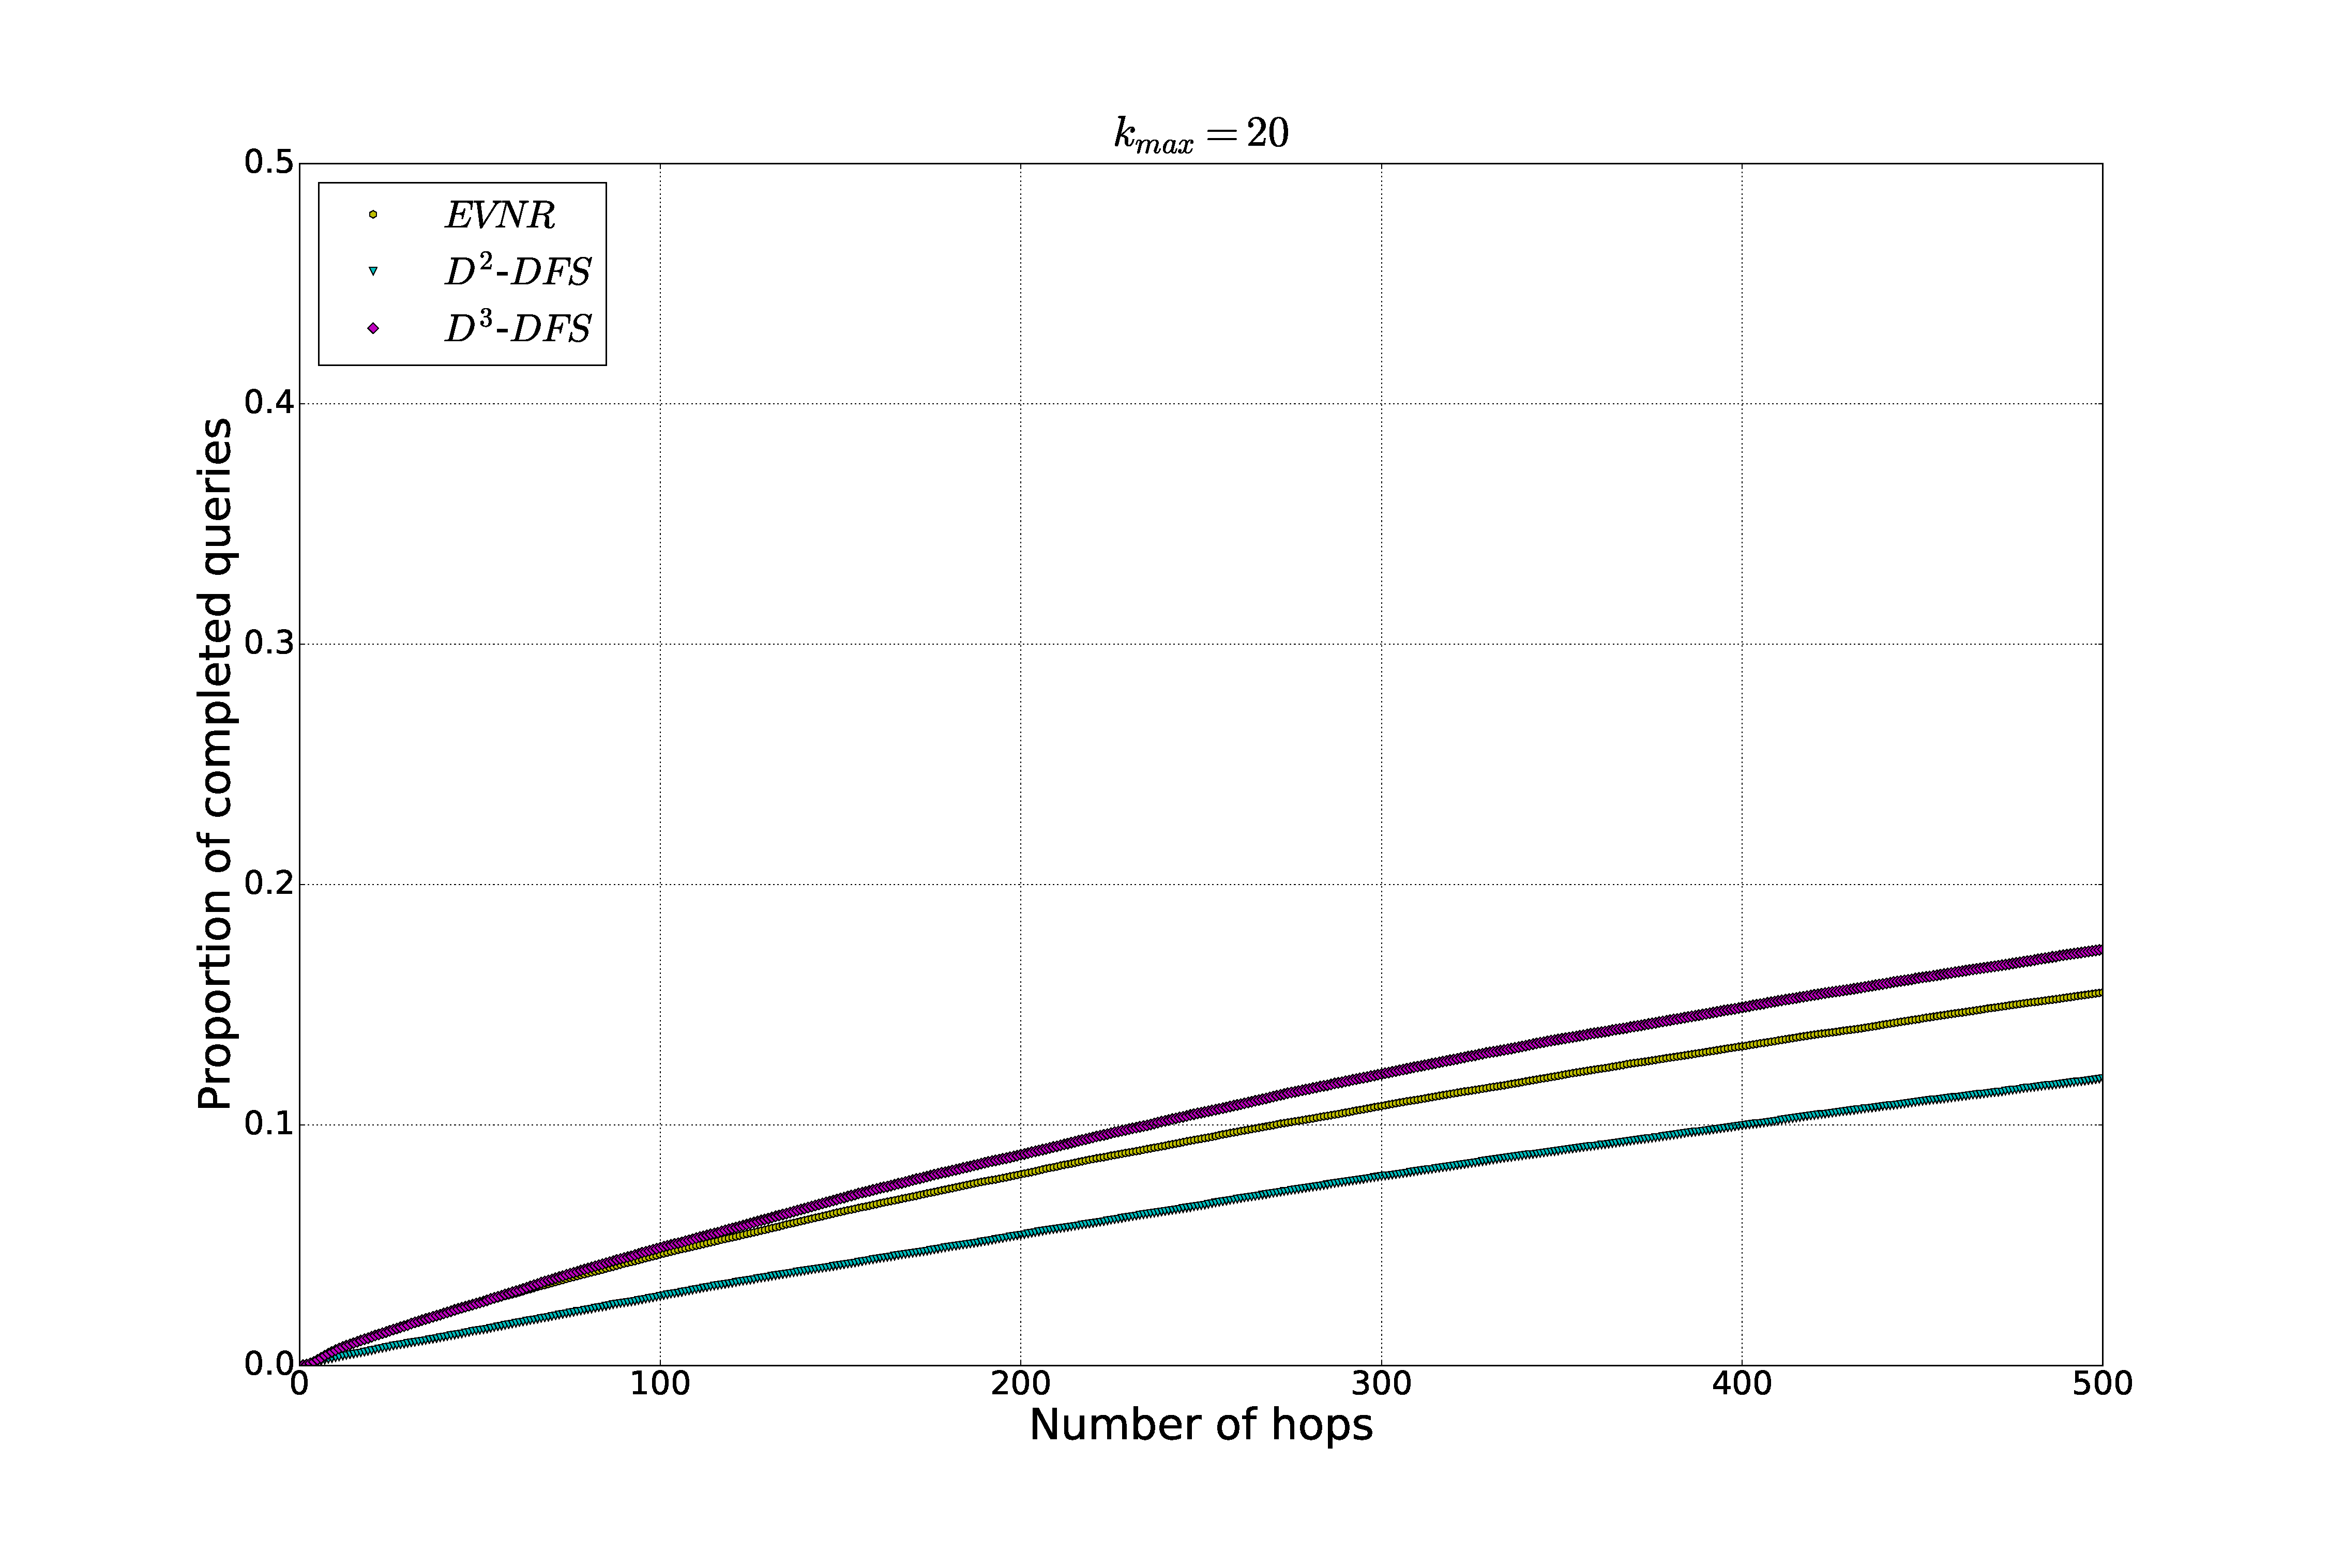
\includegraphics[width=47mm]{../fig/cml_20clip.eps}
     \end{center}
     \label{fig:12}
    \end{minipage}\begin{minipage}{0.33\hsize}
     \begin{center}
      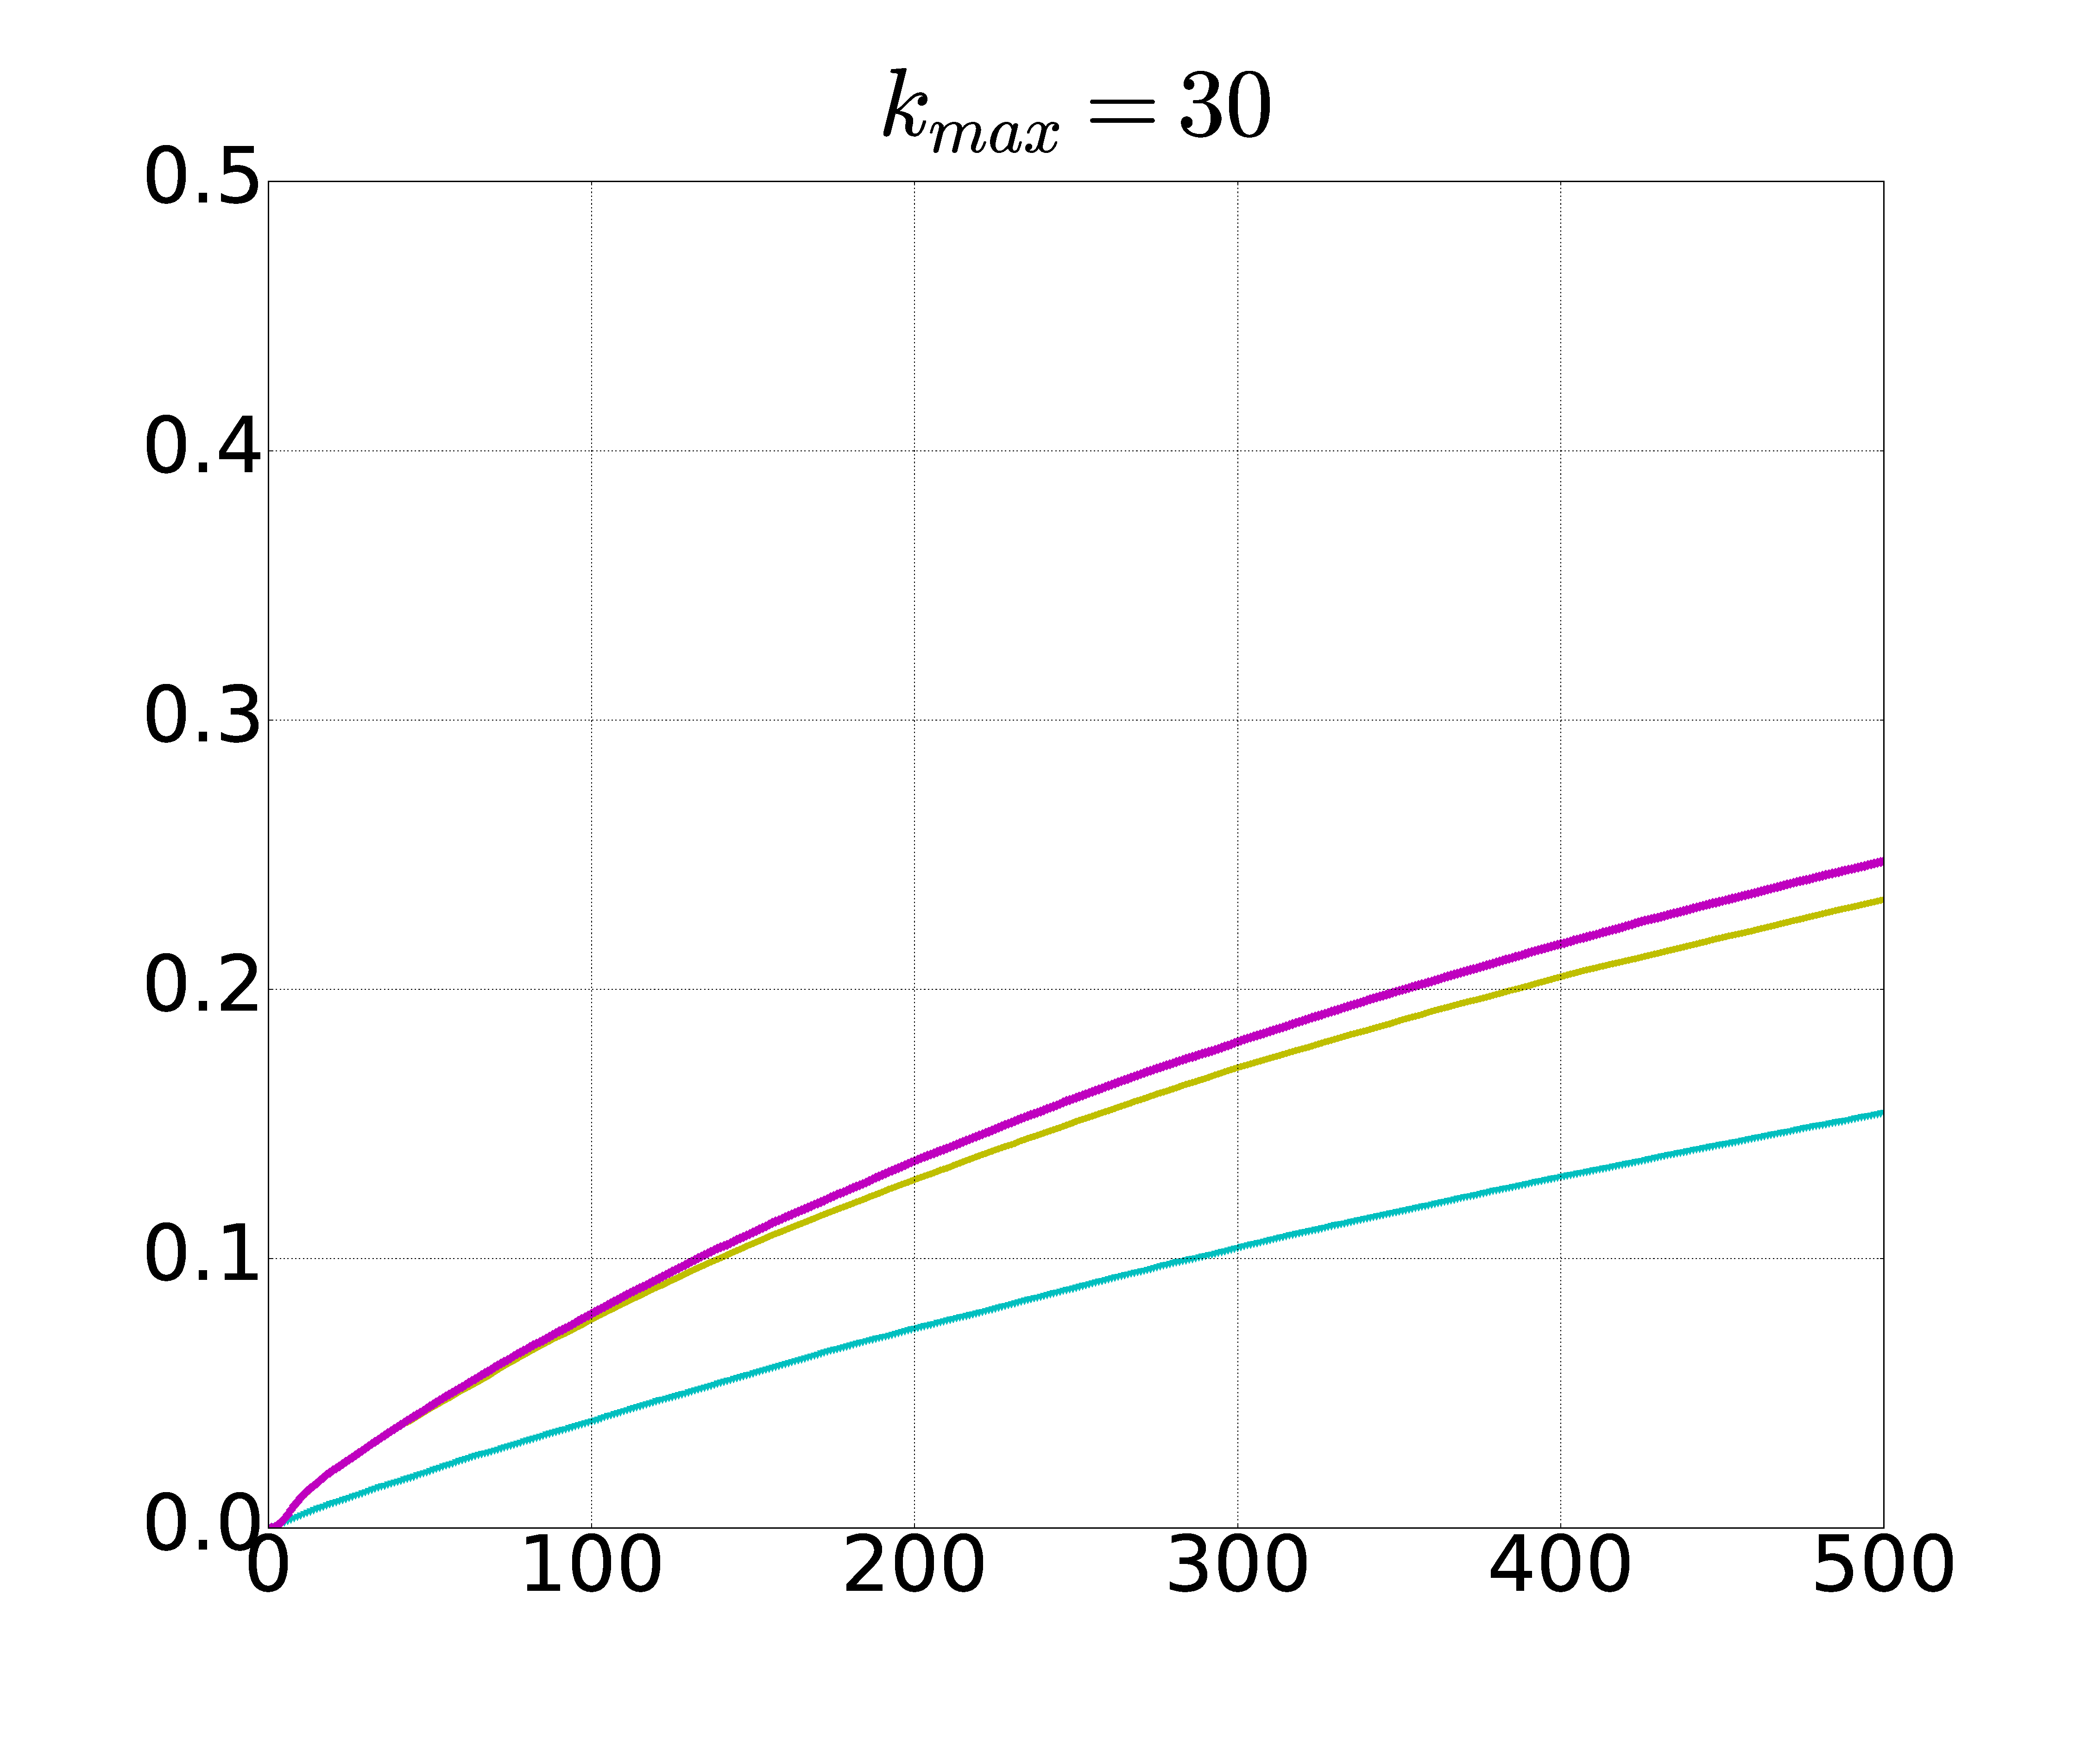
\includegraphics[width=47mm]{../fig/cml_30clip.eps}
     \end{center}
     \label{fig:13}
    \end{minipage}
    %%%%%%%%%%%%%%%%%%%%%%%%%%%%%%%%%%%%%%%%%%%%%%%%%%%%%%
    \begin{minipage}{0.33\hsize}
     \begin{center}
      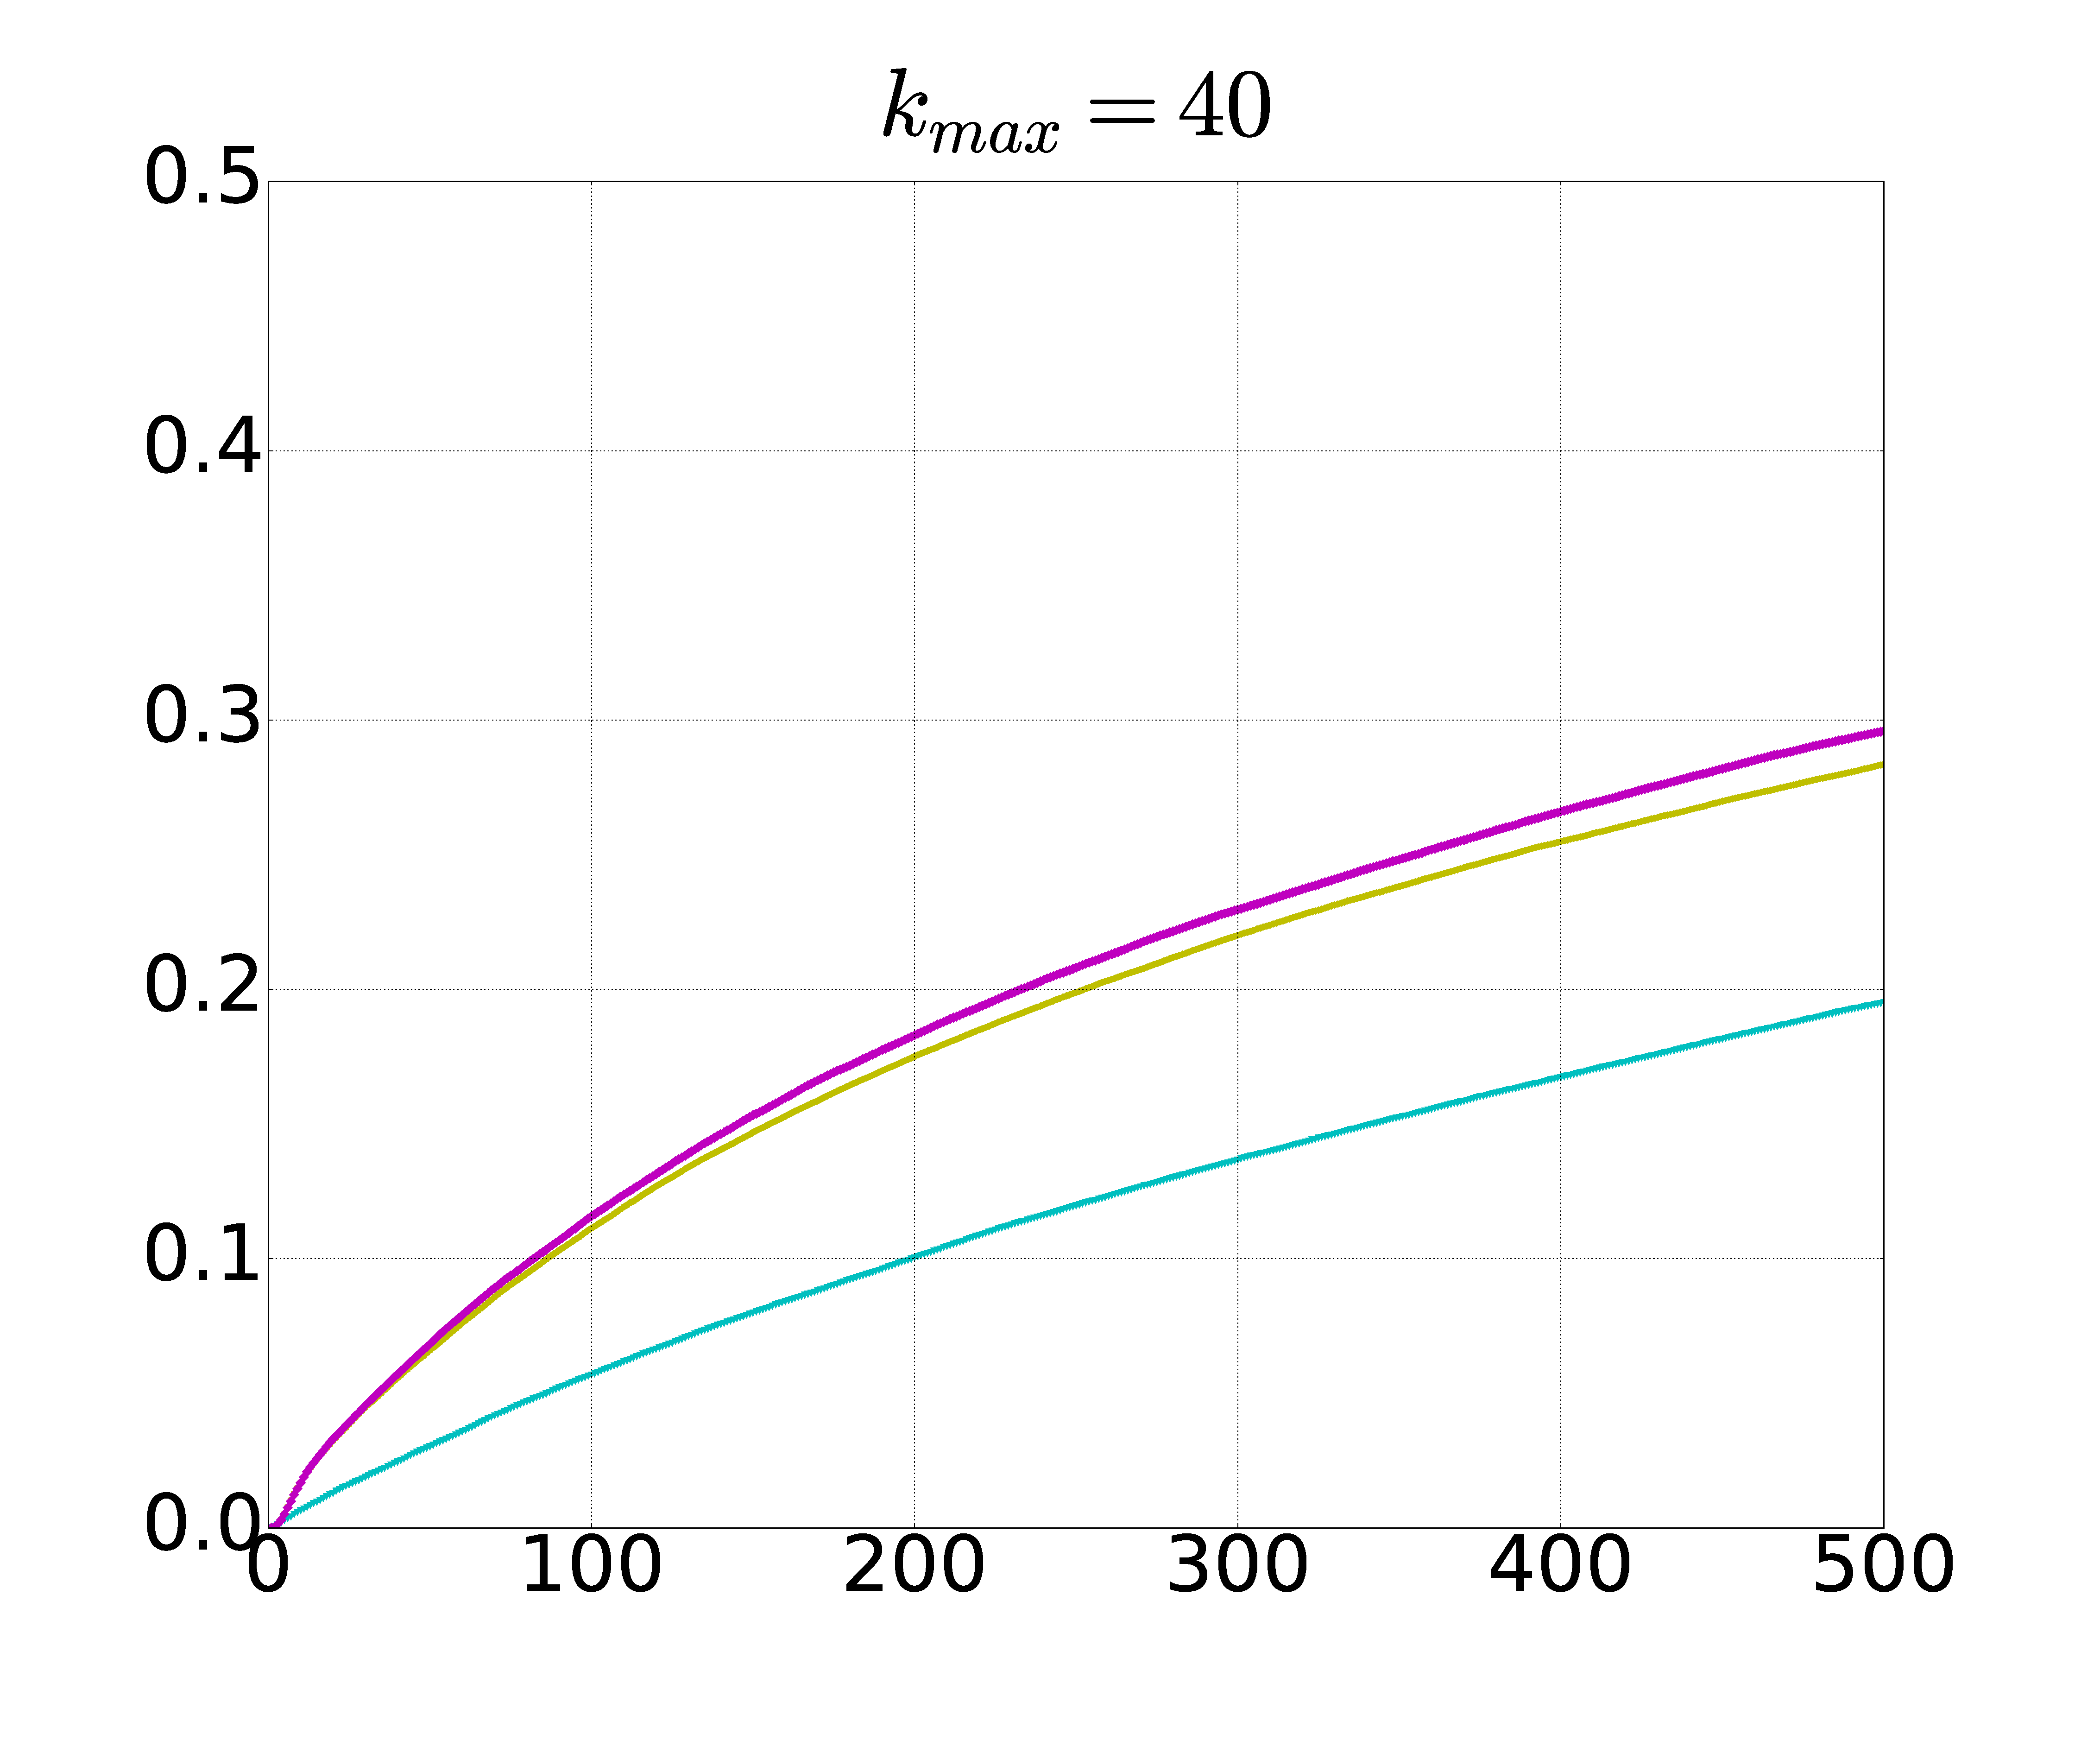
\includegraphics[width=47mm]{../fig/cml_40clip.eps}
     \end{center}
     \label{fig:21}
    \end{minipage}\begin{minipage}{0.33\hsize}
     \begin{center}
      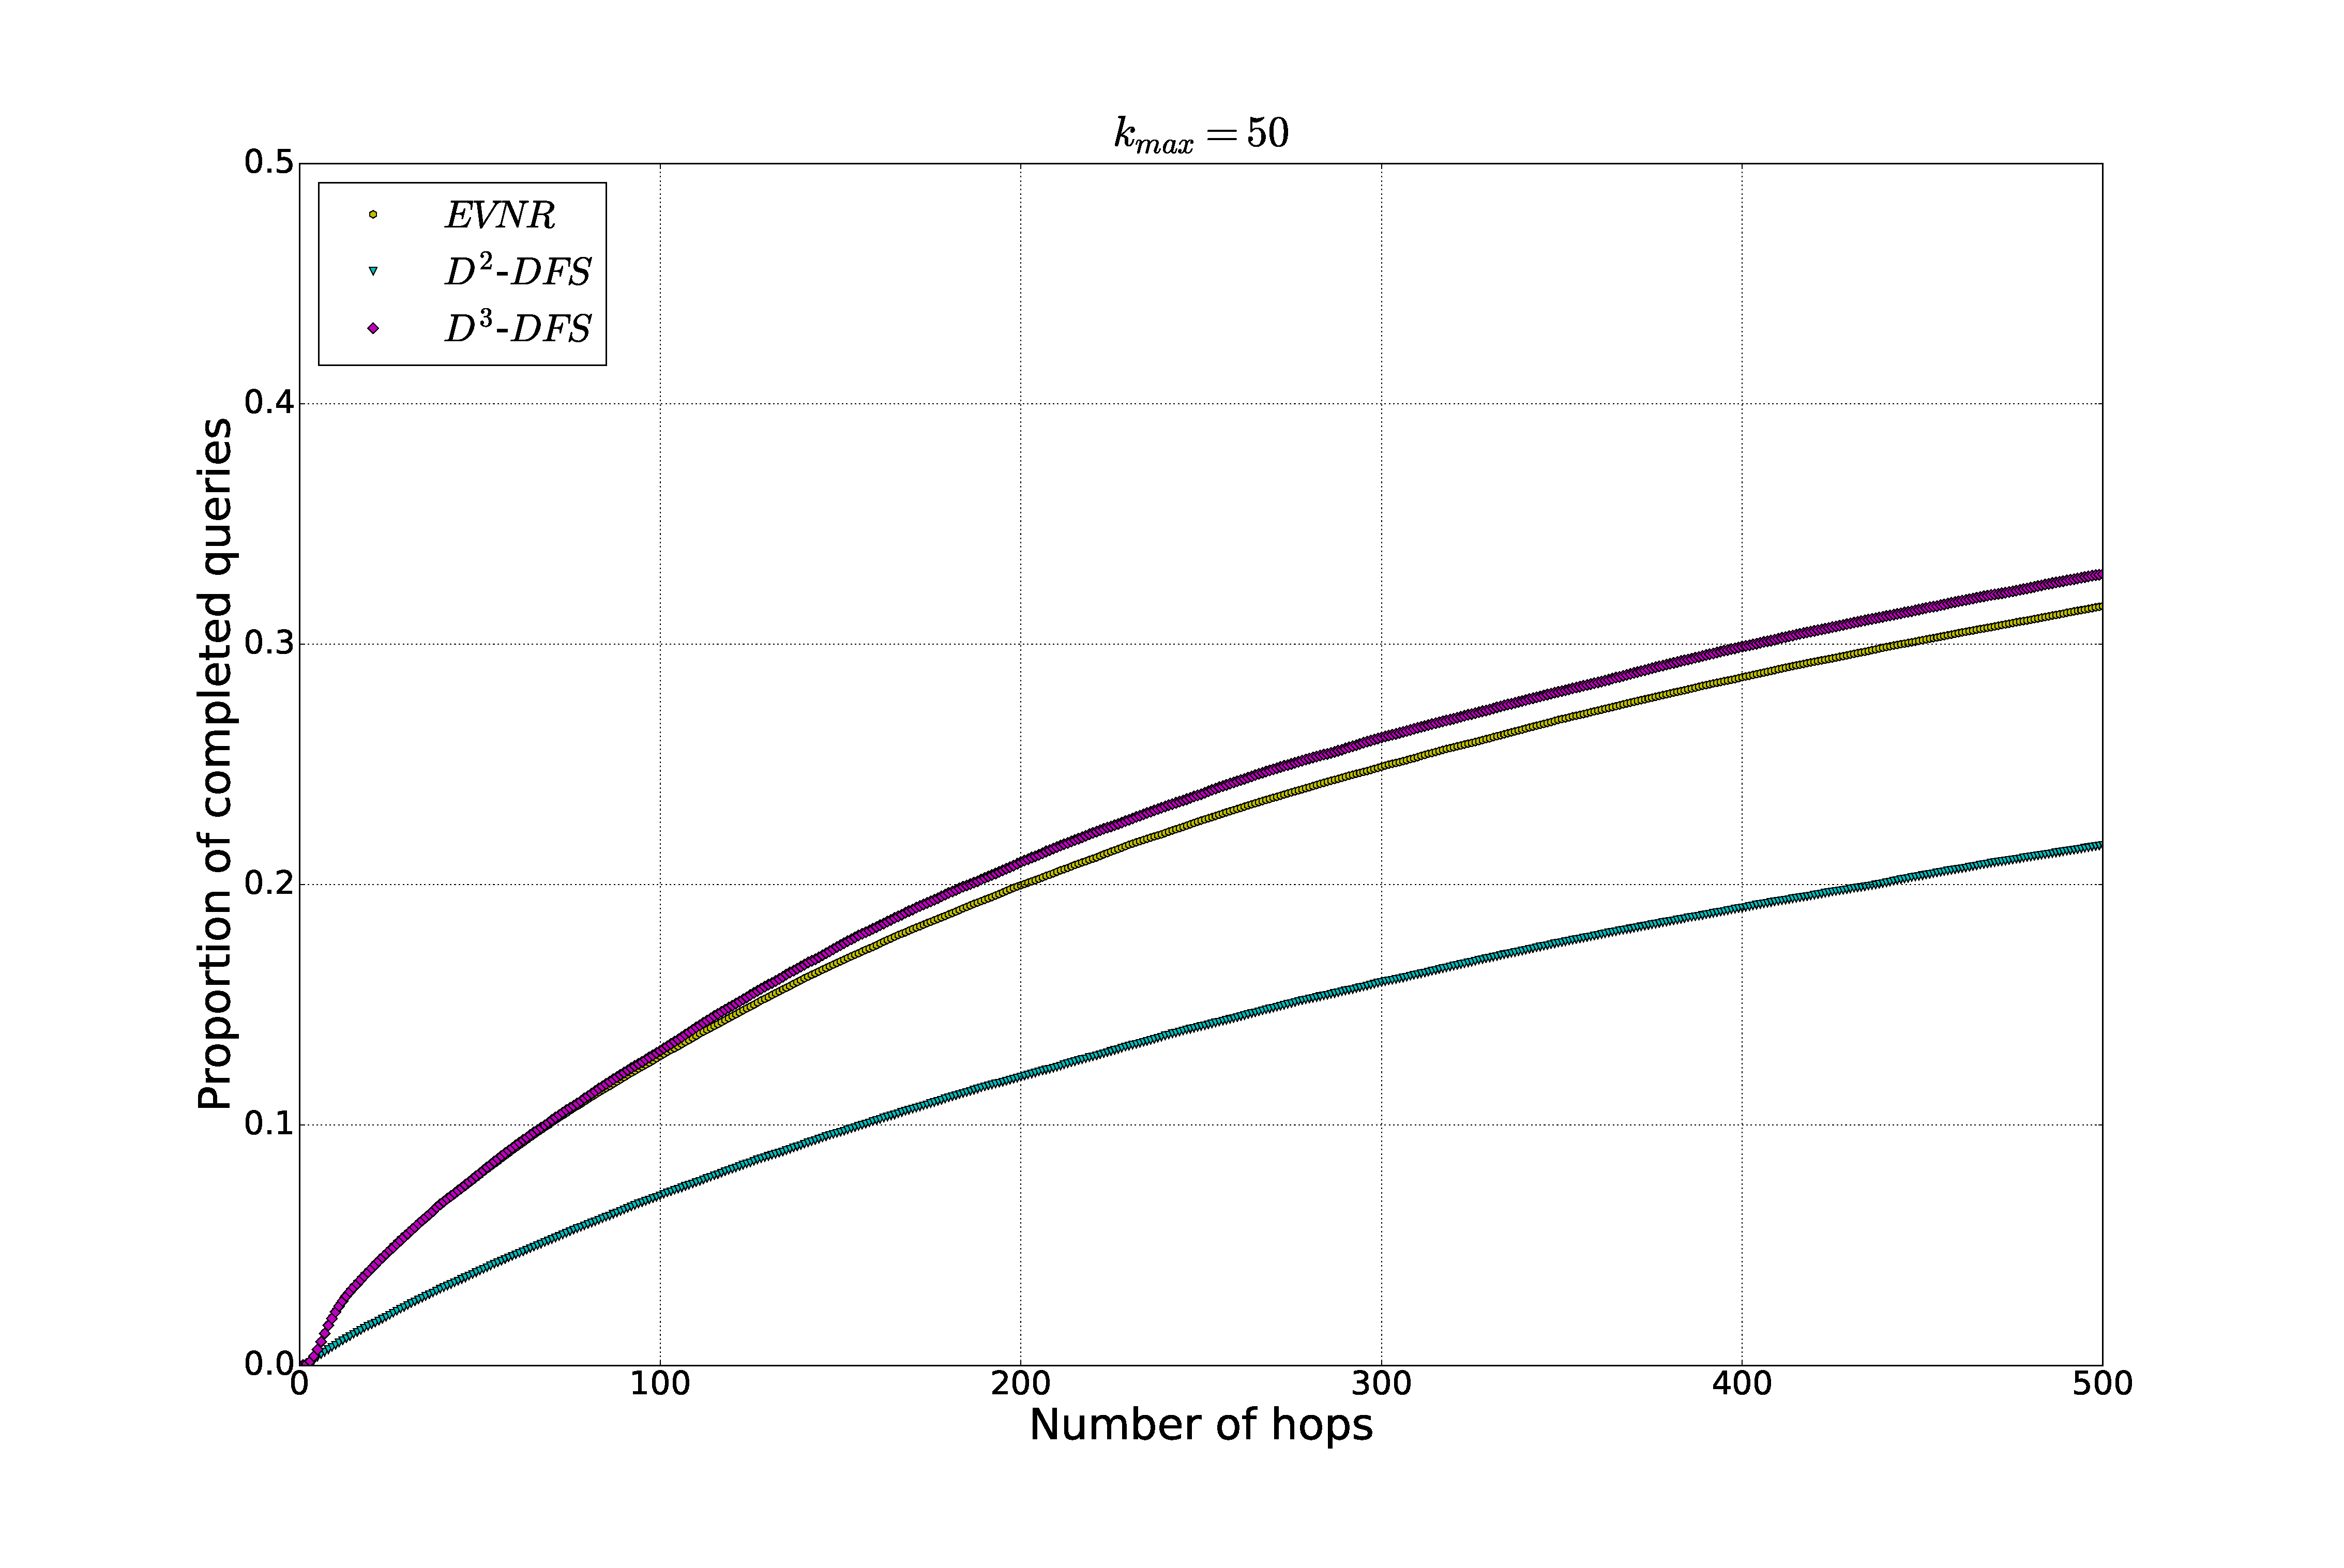
\includegraphics[width=47mm]{../fig/cml_50clip.eps}
     \end{center}
     \label{fig:22}
    \end{minipage}\begin{minipage}{0.33\hsize}
     \begin{center}
      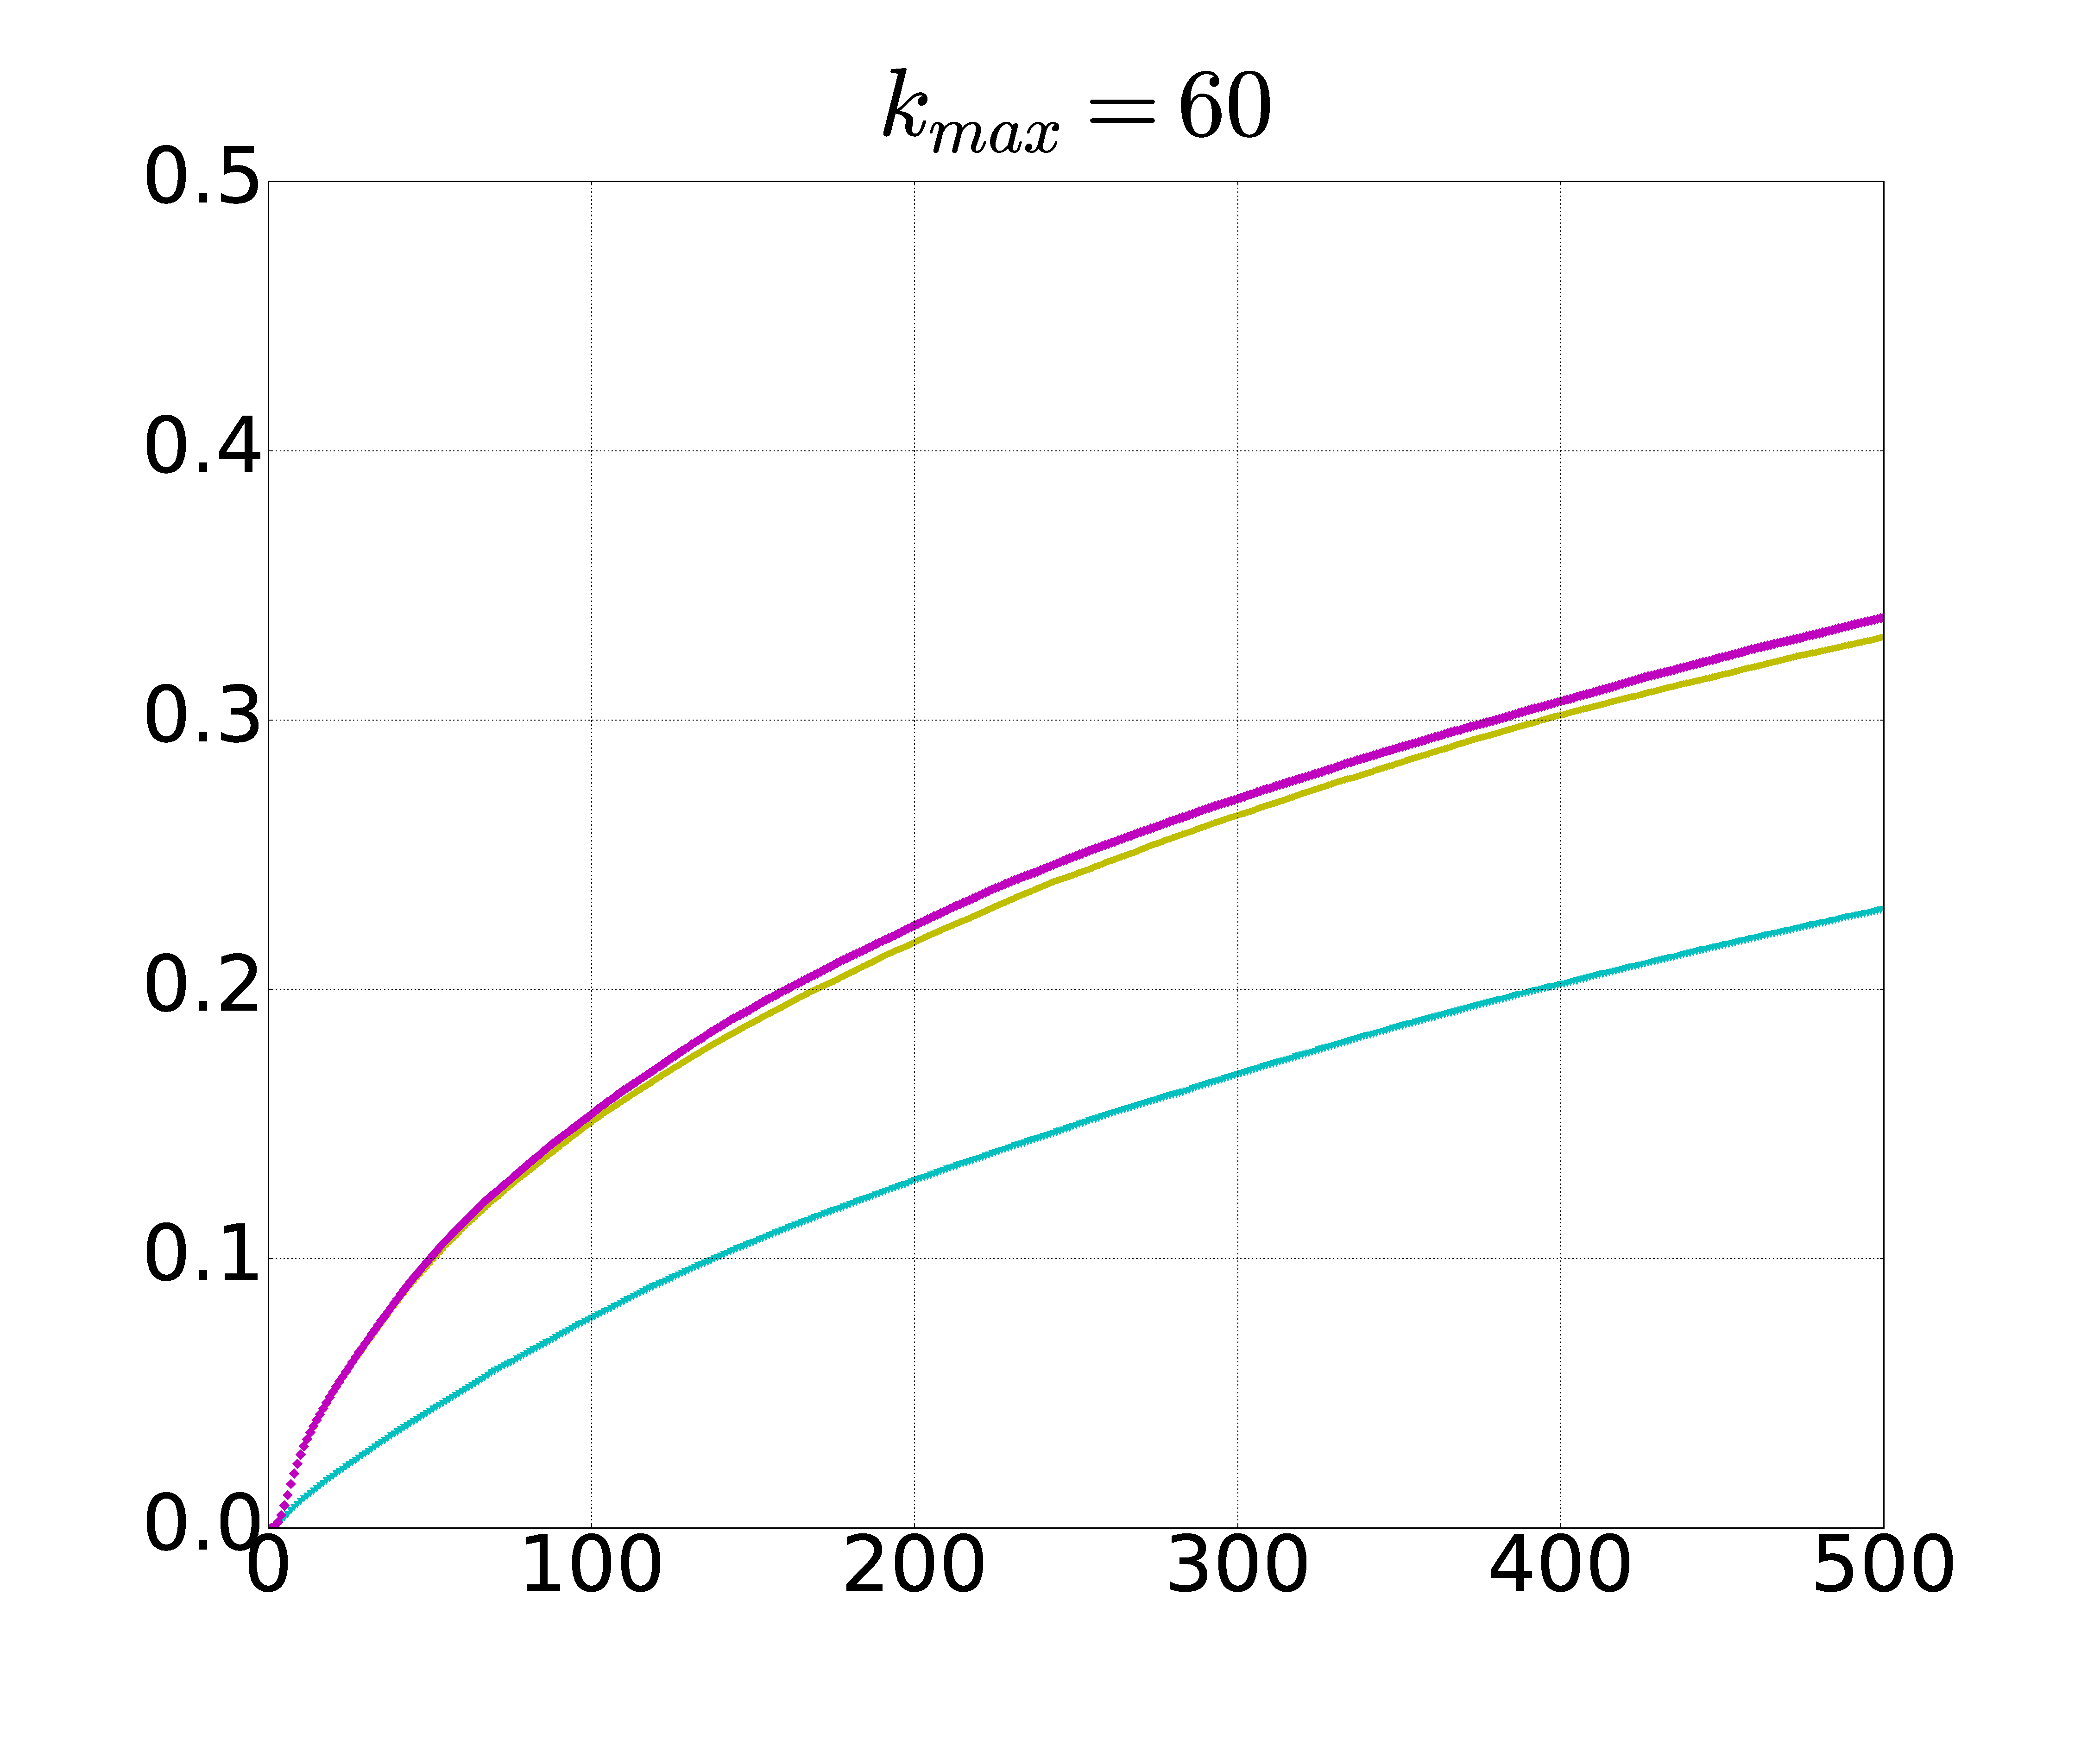
\includegraphics[width=47mm]{../fig/cml_60clip.eps}
     \end{center}
     \label{fig:23}
    \end{minipage}
    %%%%%%%%%%%%%%%%%%%%%%%%%%%%%%%%%%%%%%%%%%%%%%%%%%%%%%
    \begin{minipage}{0.33\hsize}
     \begin{center}
      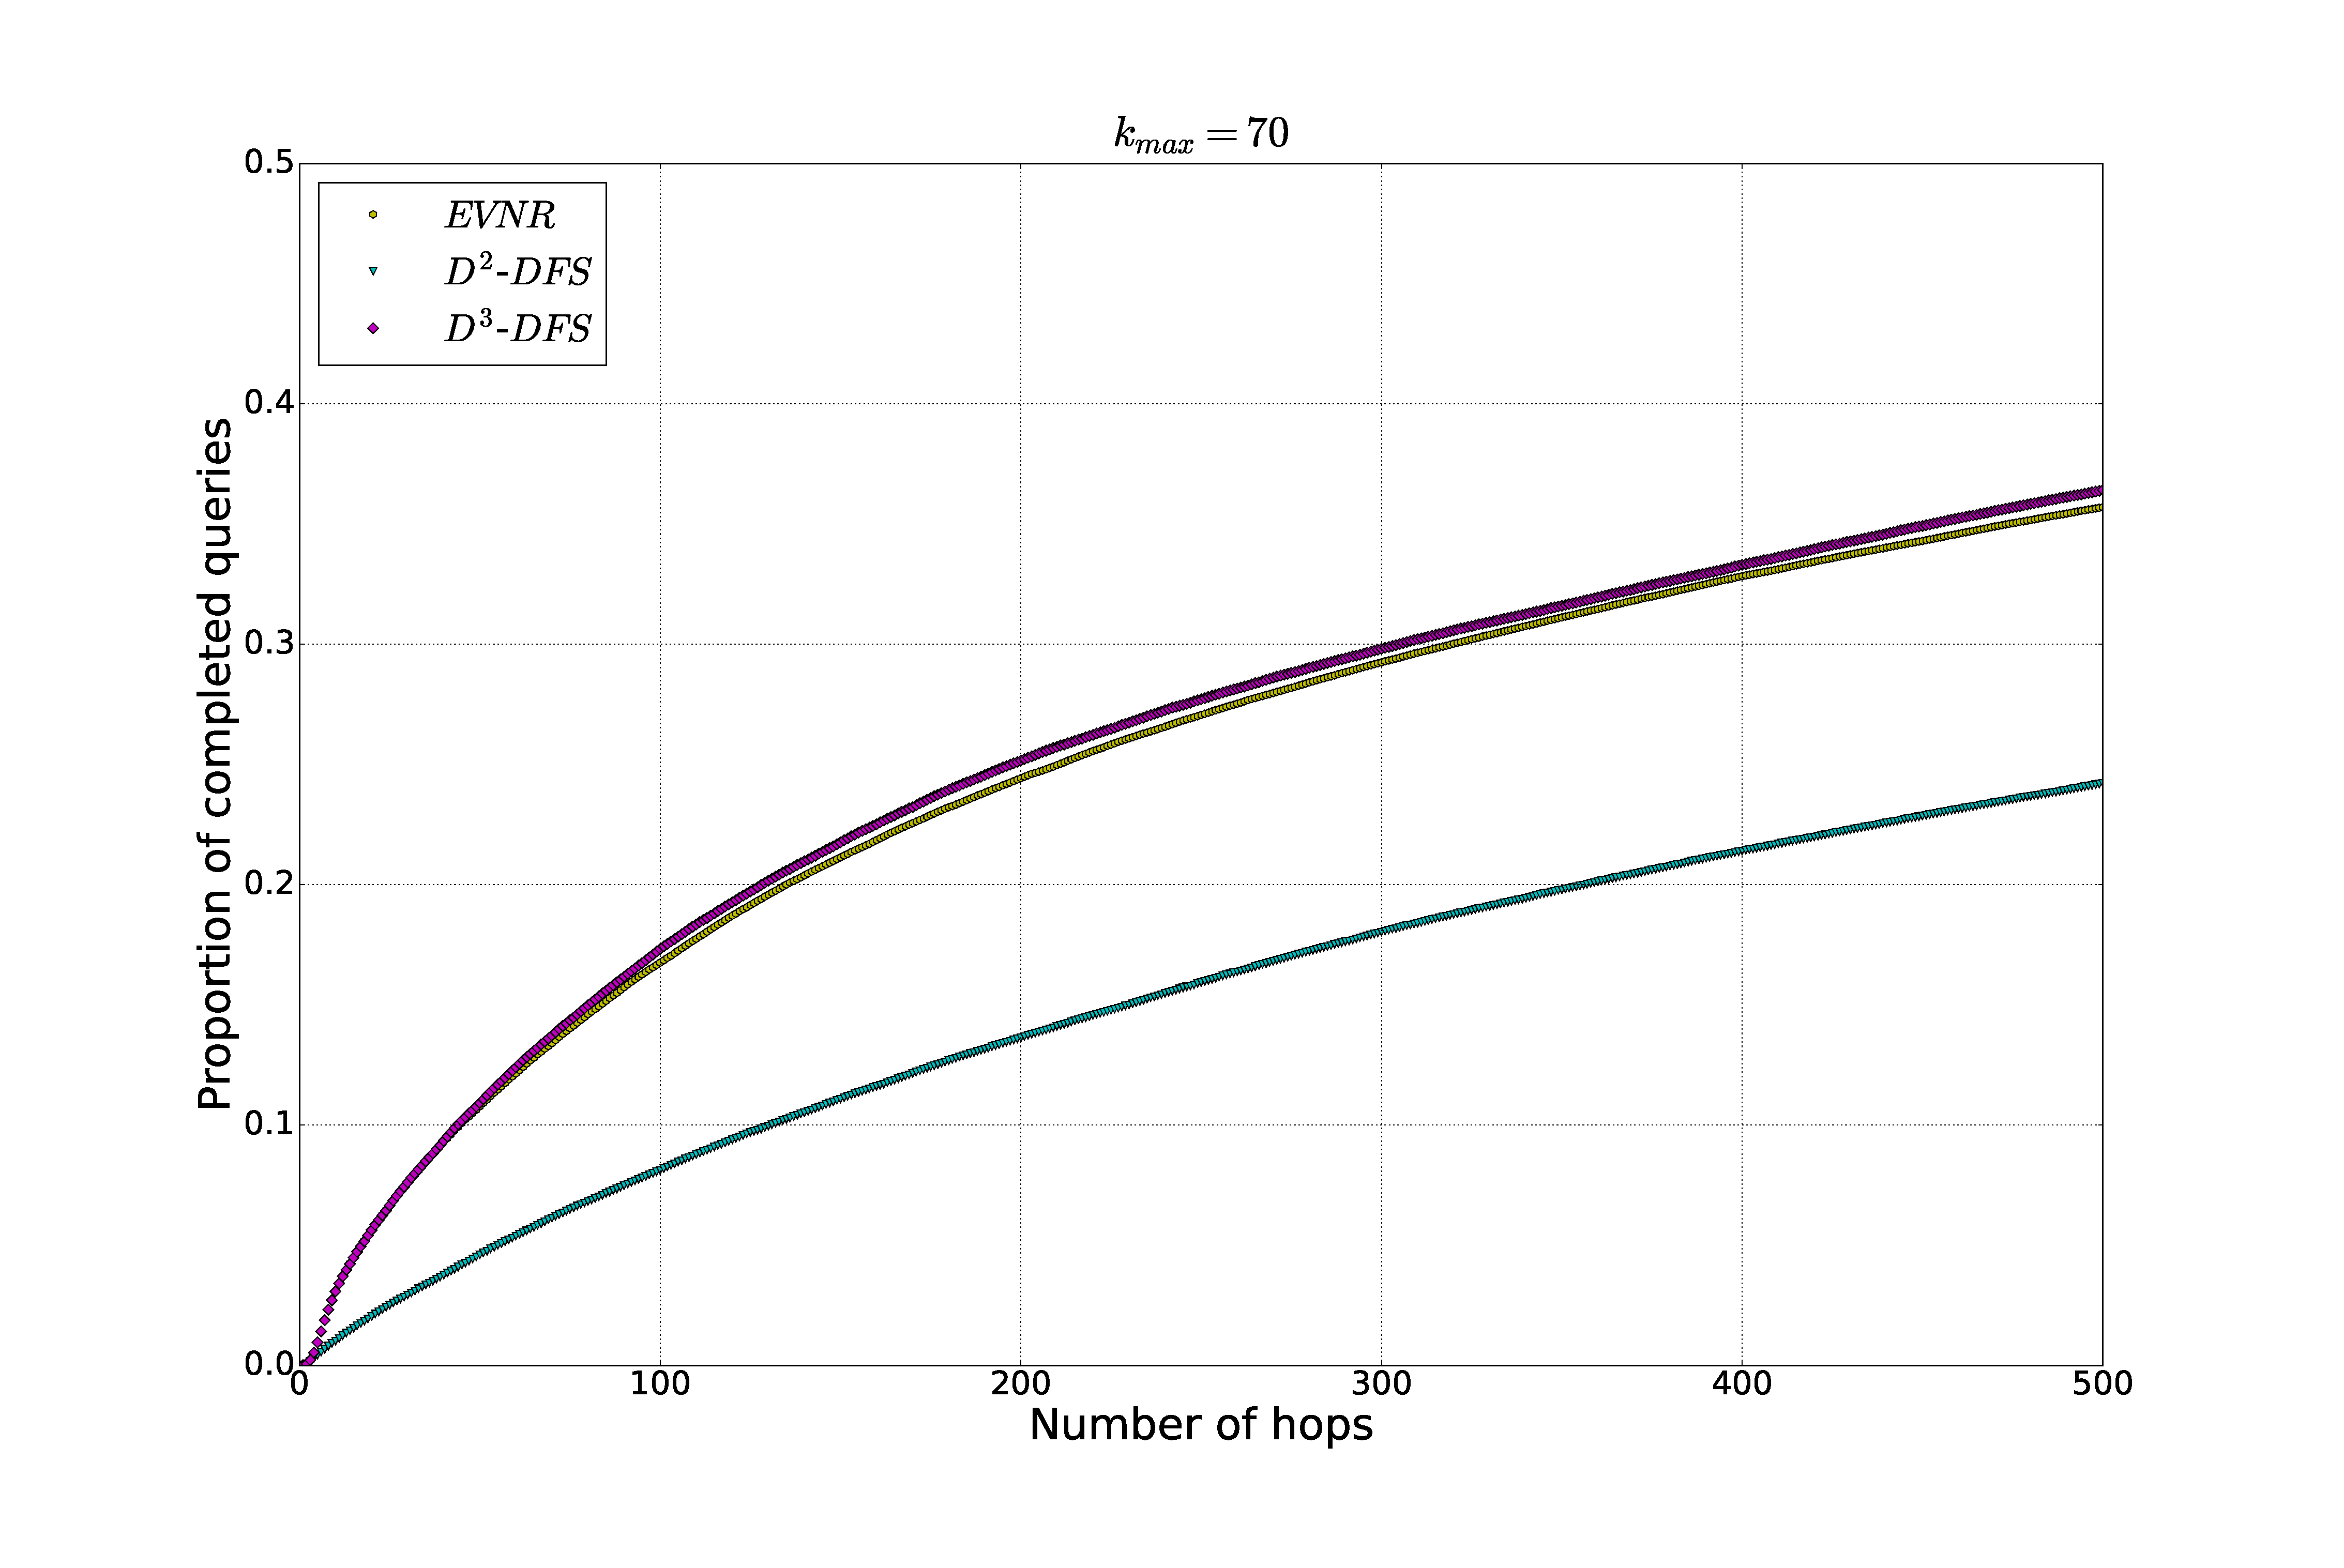
\includegraphics[width=47mm]{../fig/cml_70clip.eps}
     \end{center}
     \label{fig:31}
    \end{minipage}\begin{minipage}{0.33\hsize}
     \begin{center}
      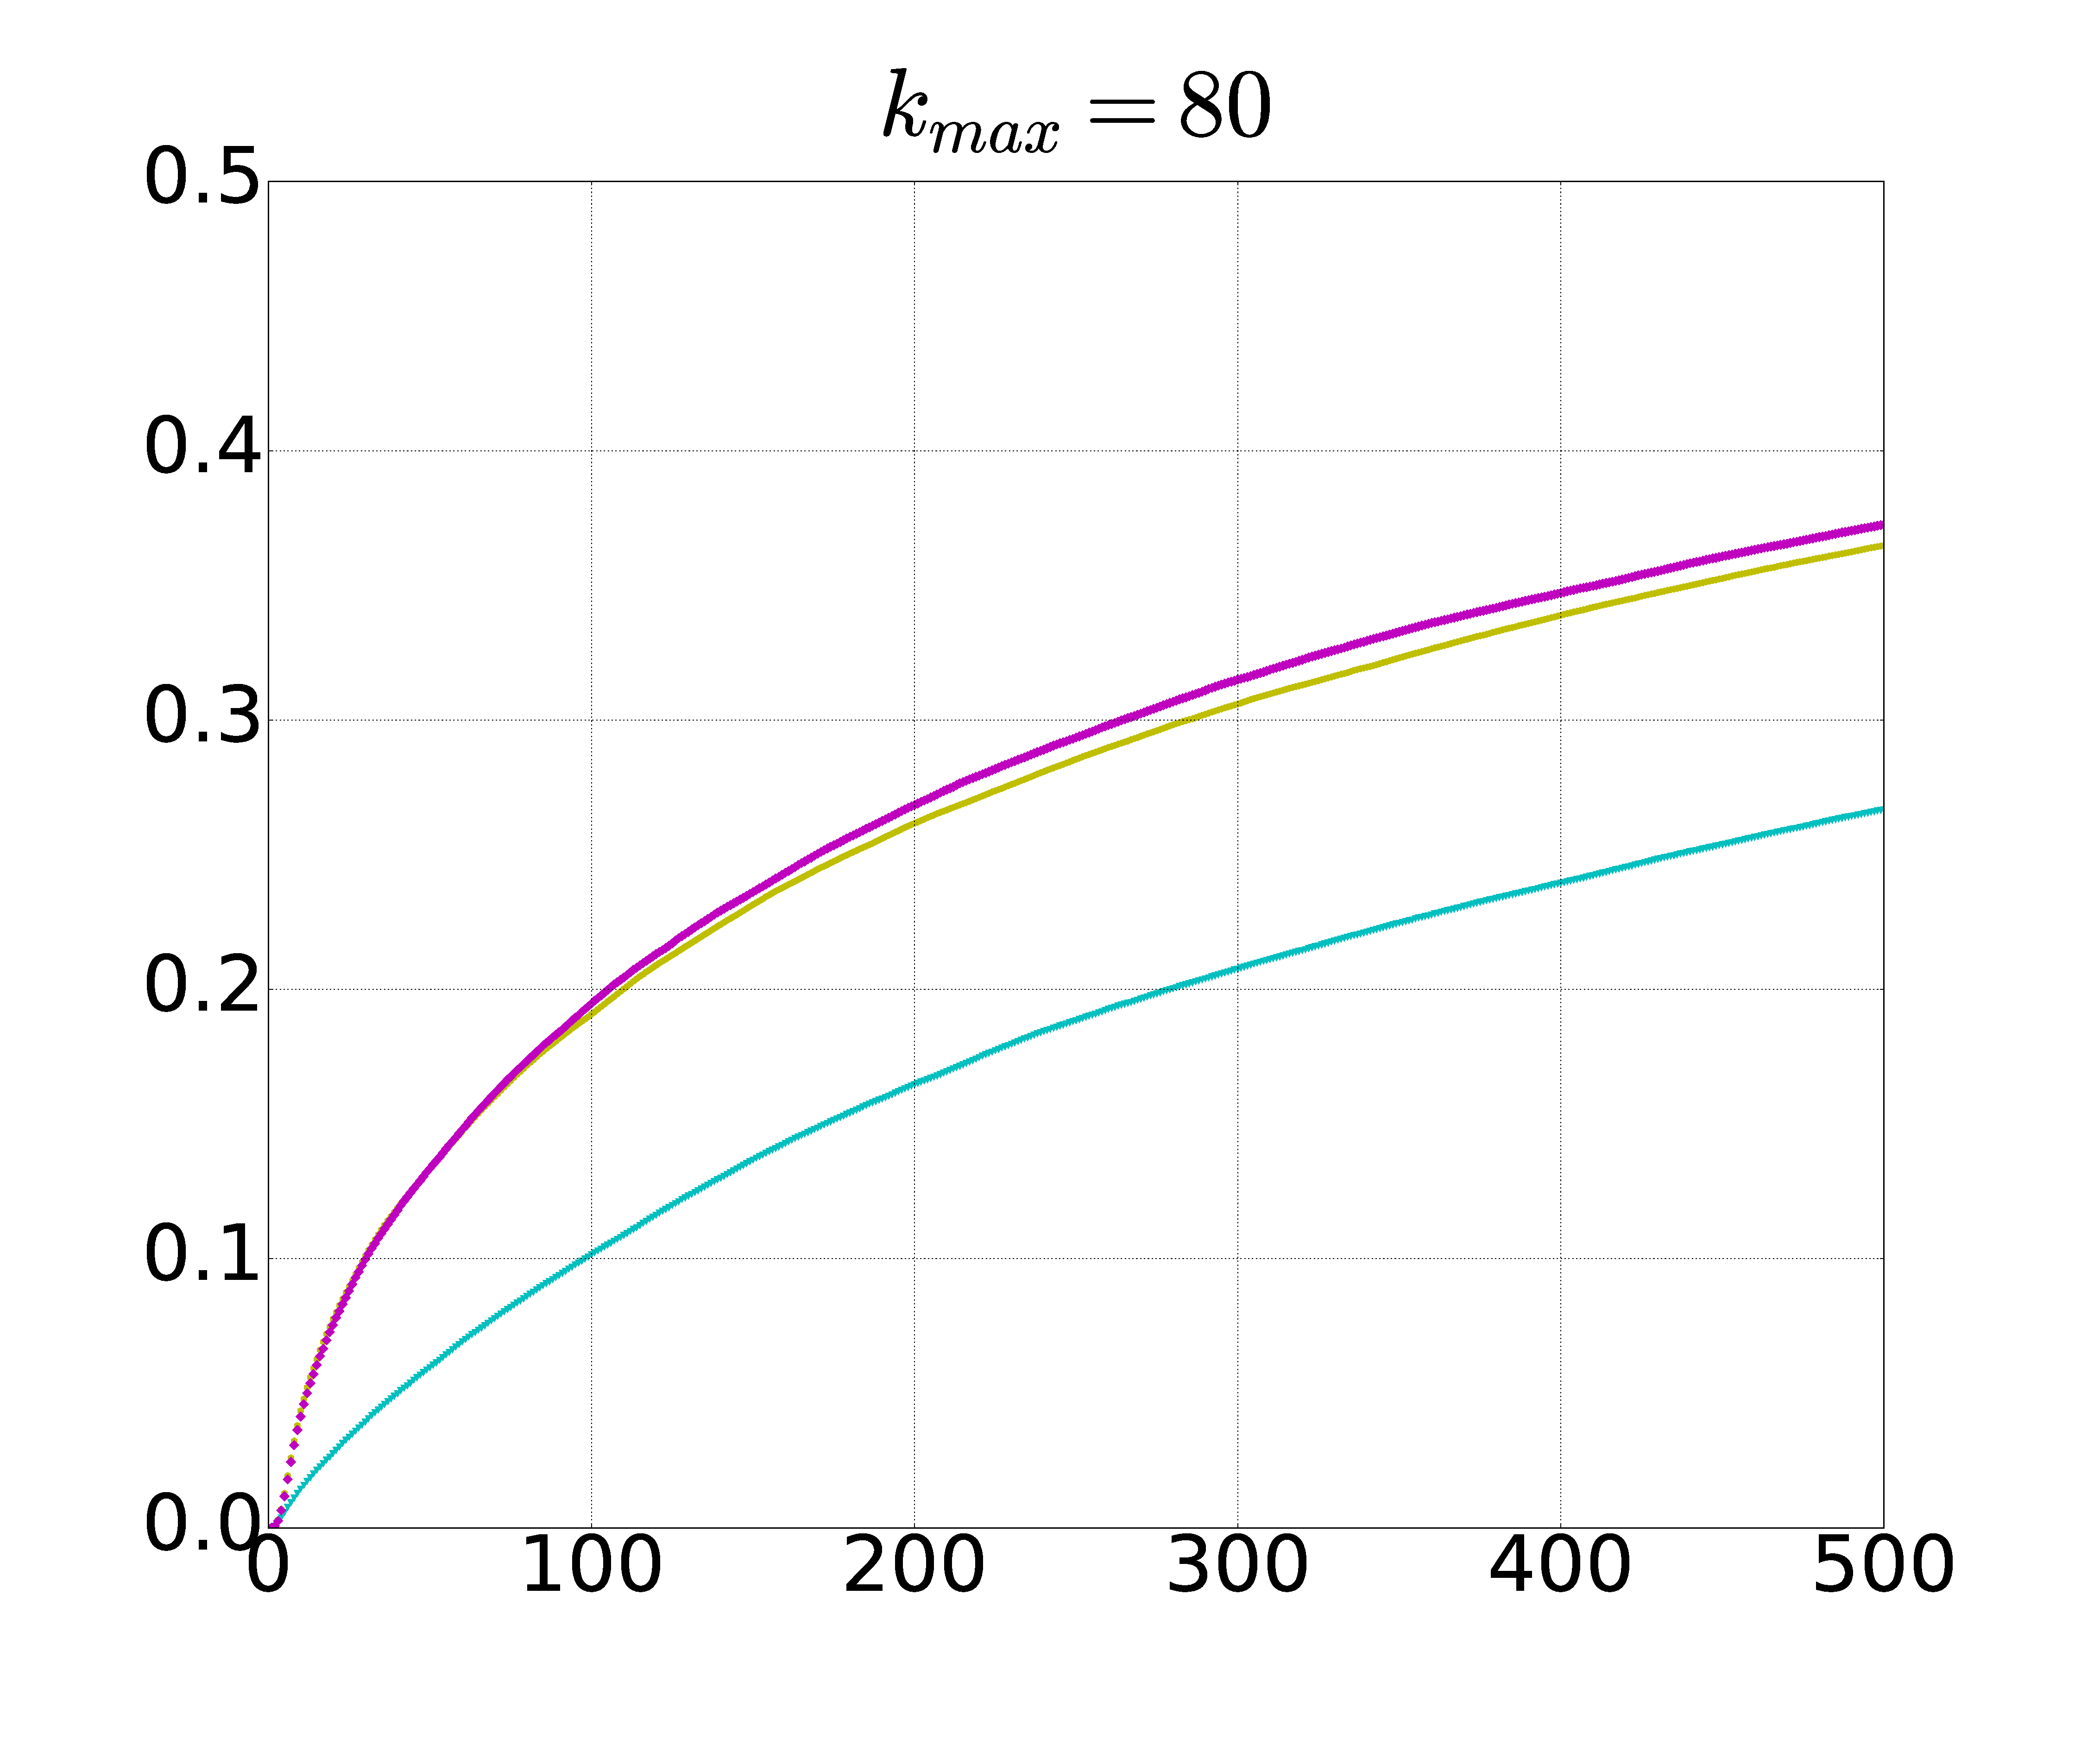
\includegraphics[width=47mm]{../fig/cml_80clip.eps}
     \end{center}
     \label{fig:32}
    \end{minipage}\begin{minipage}{0.33\hsize}
     \begin{center}
      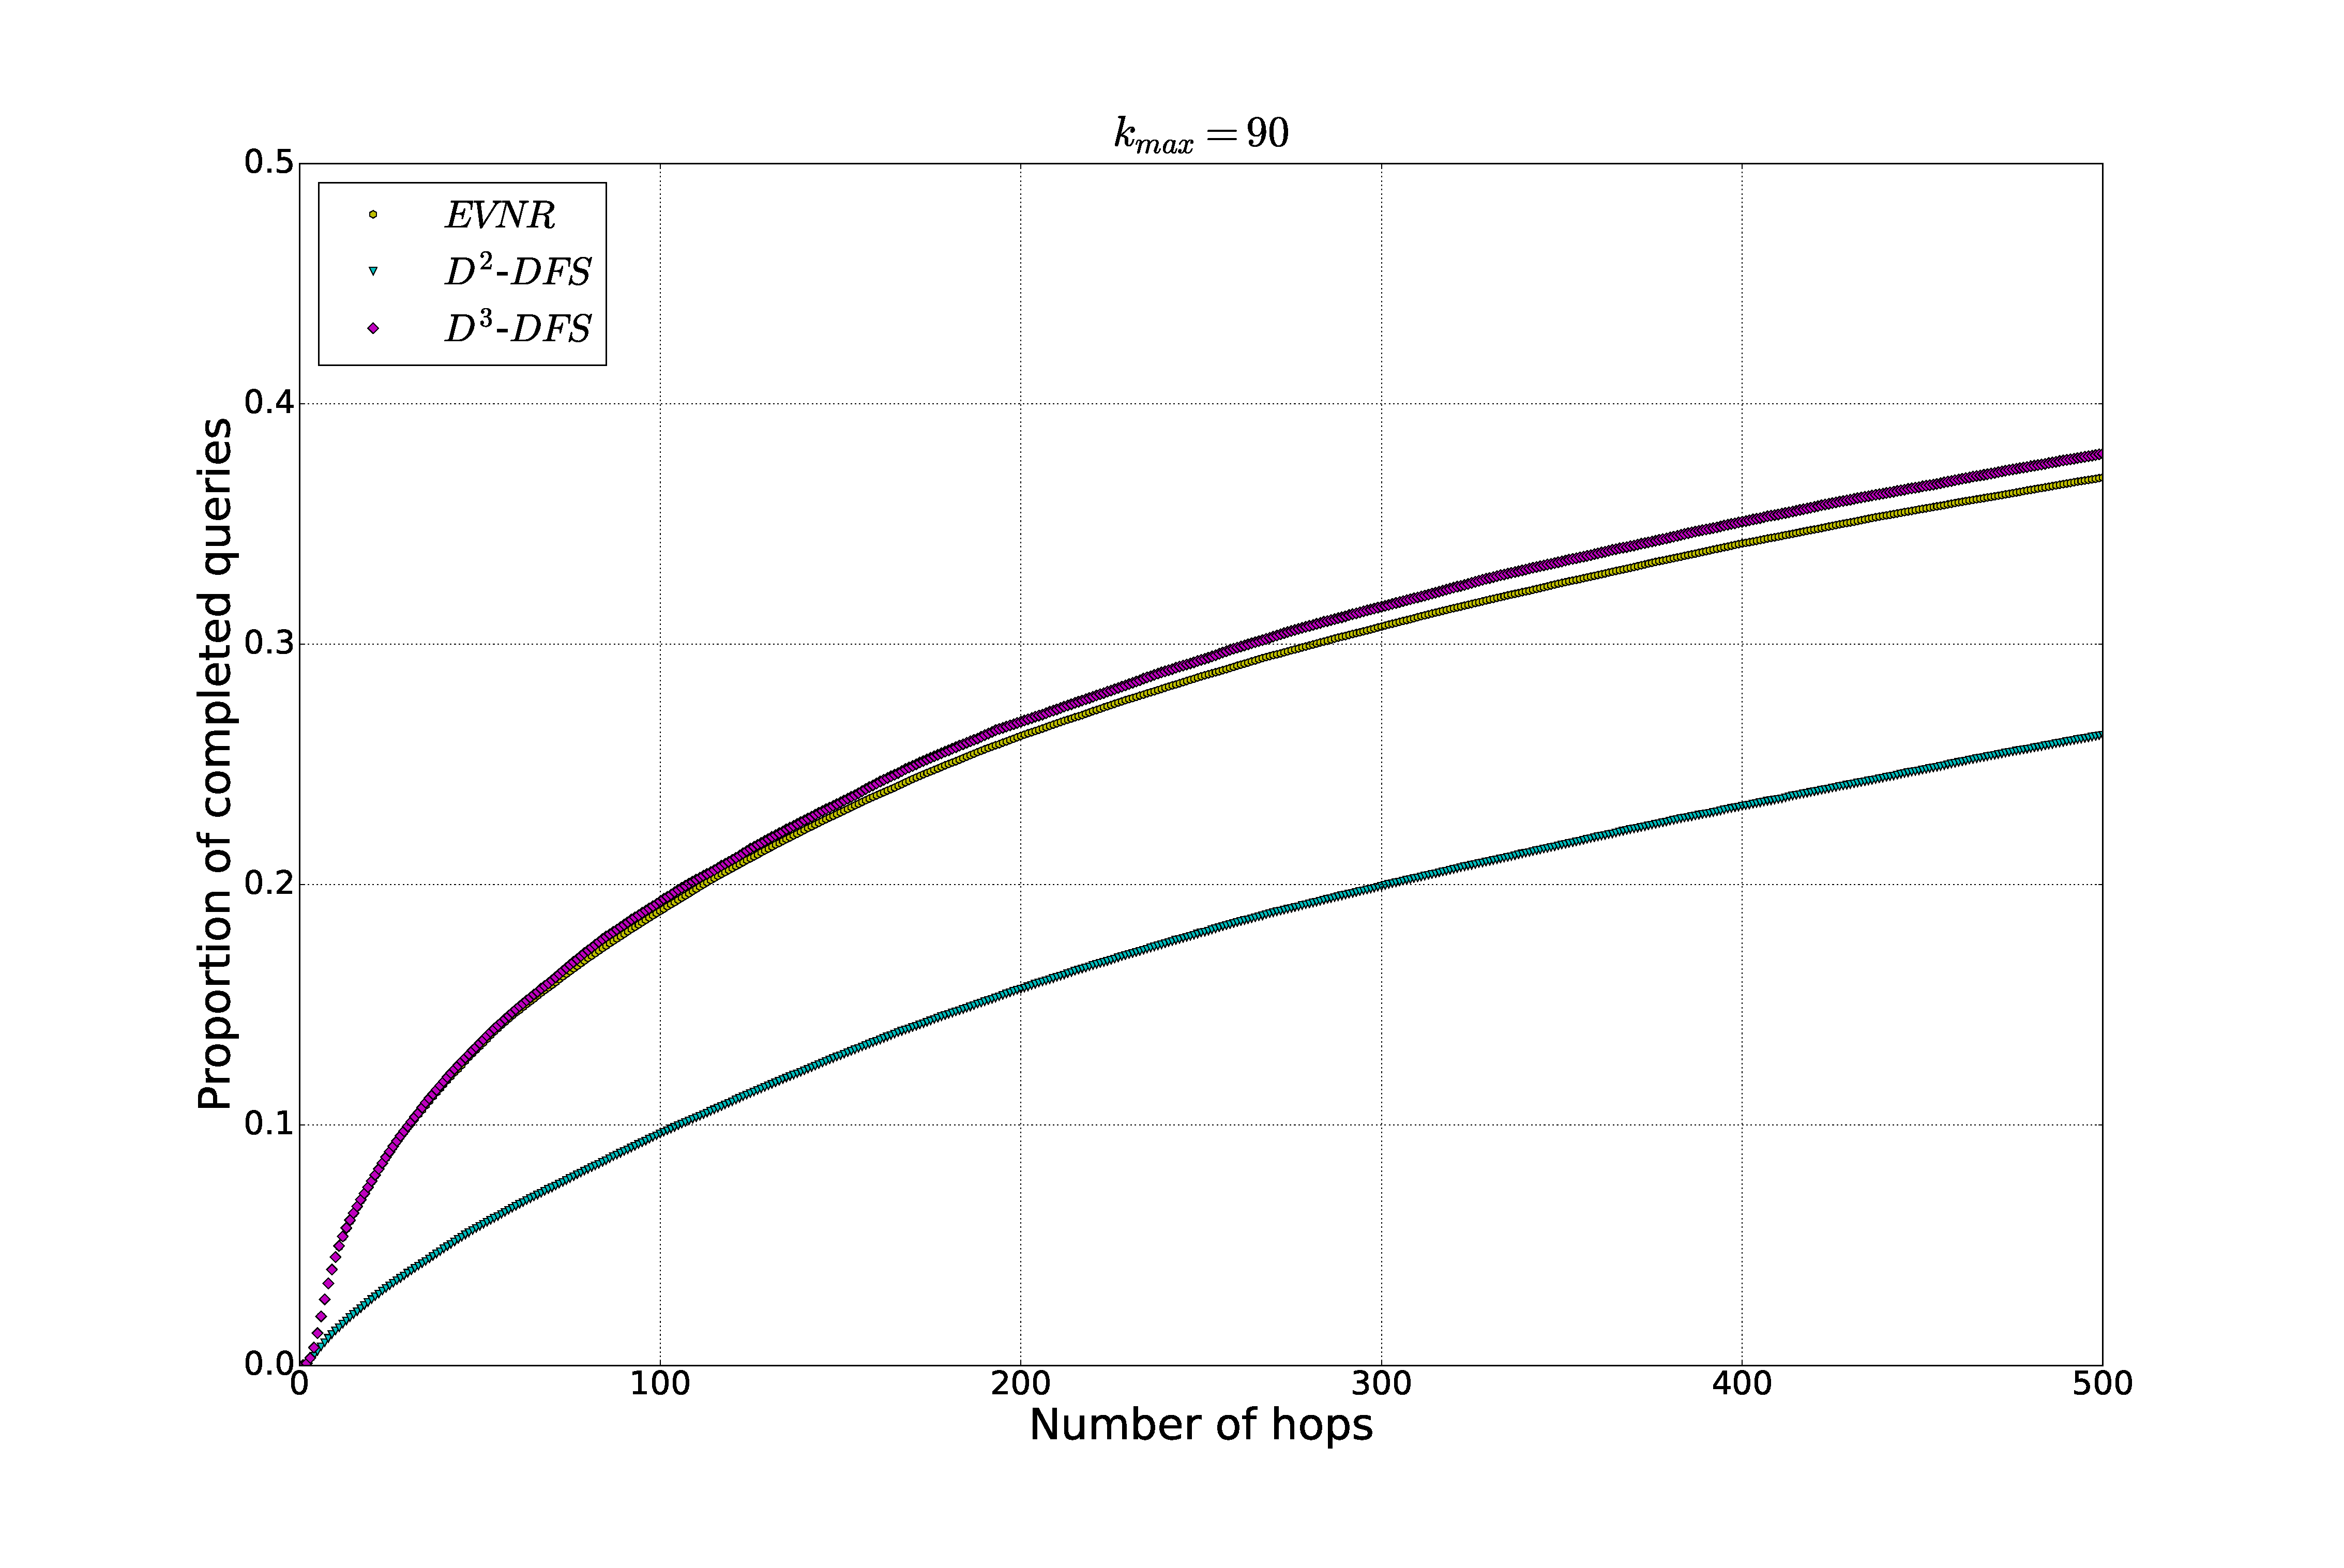
\includegraphics[width=47mm]{../fig/cml_90clip.eps}
     \end{center}
     \label{fig:33}
    \end{minipage}
    %%%%%%%%%%%%%%%%%%%%%%%%%%%%%%%%%%%%%%%%%%%%%%%%%%%%%%
    \begin{center}
     \begin{minipage}{0.33\hsize}
      \centerline{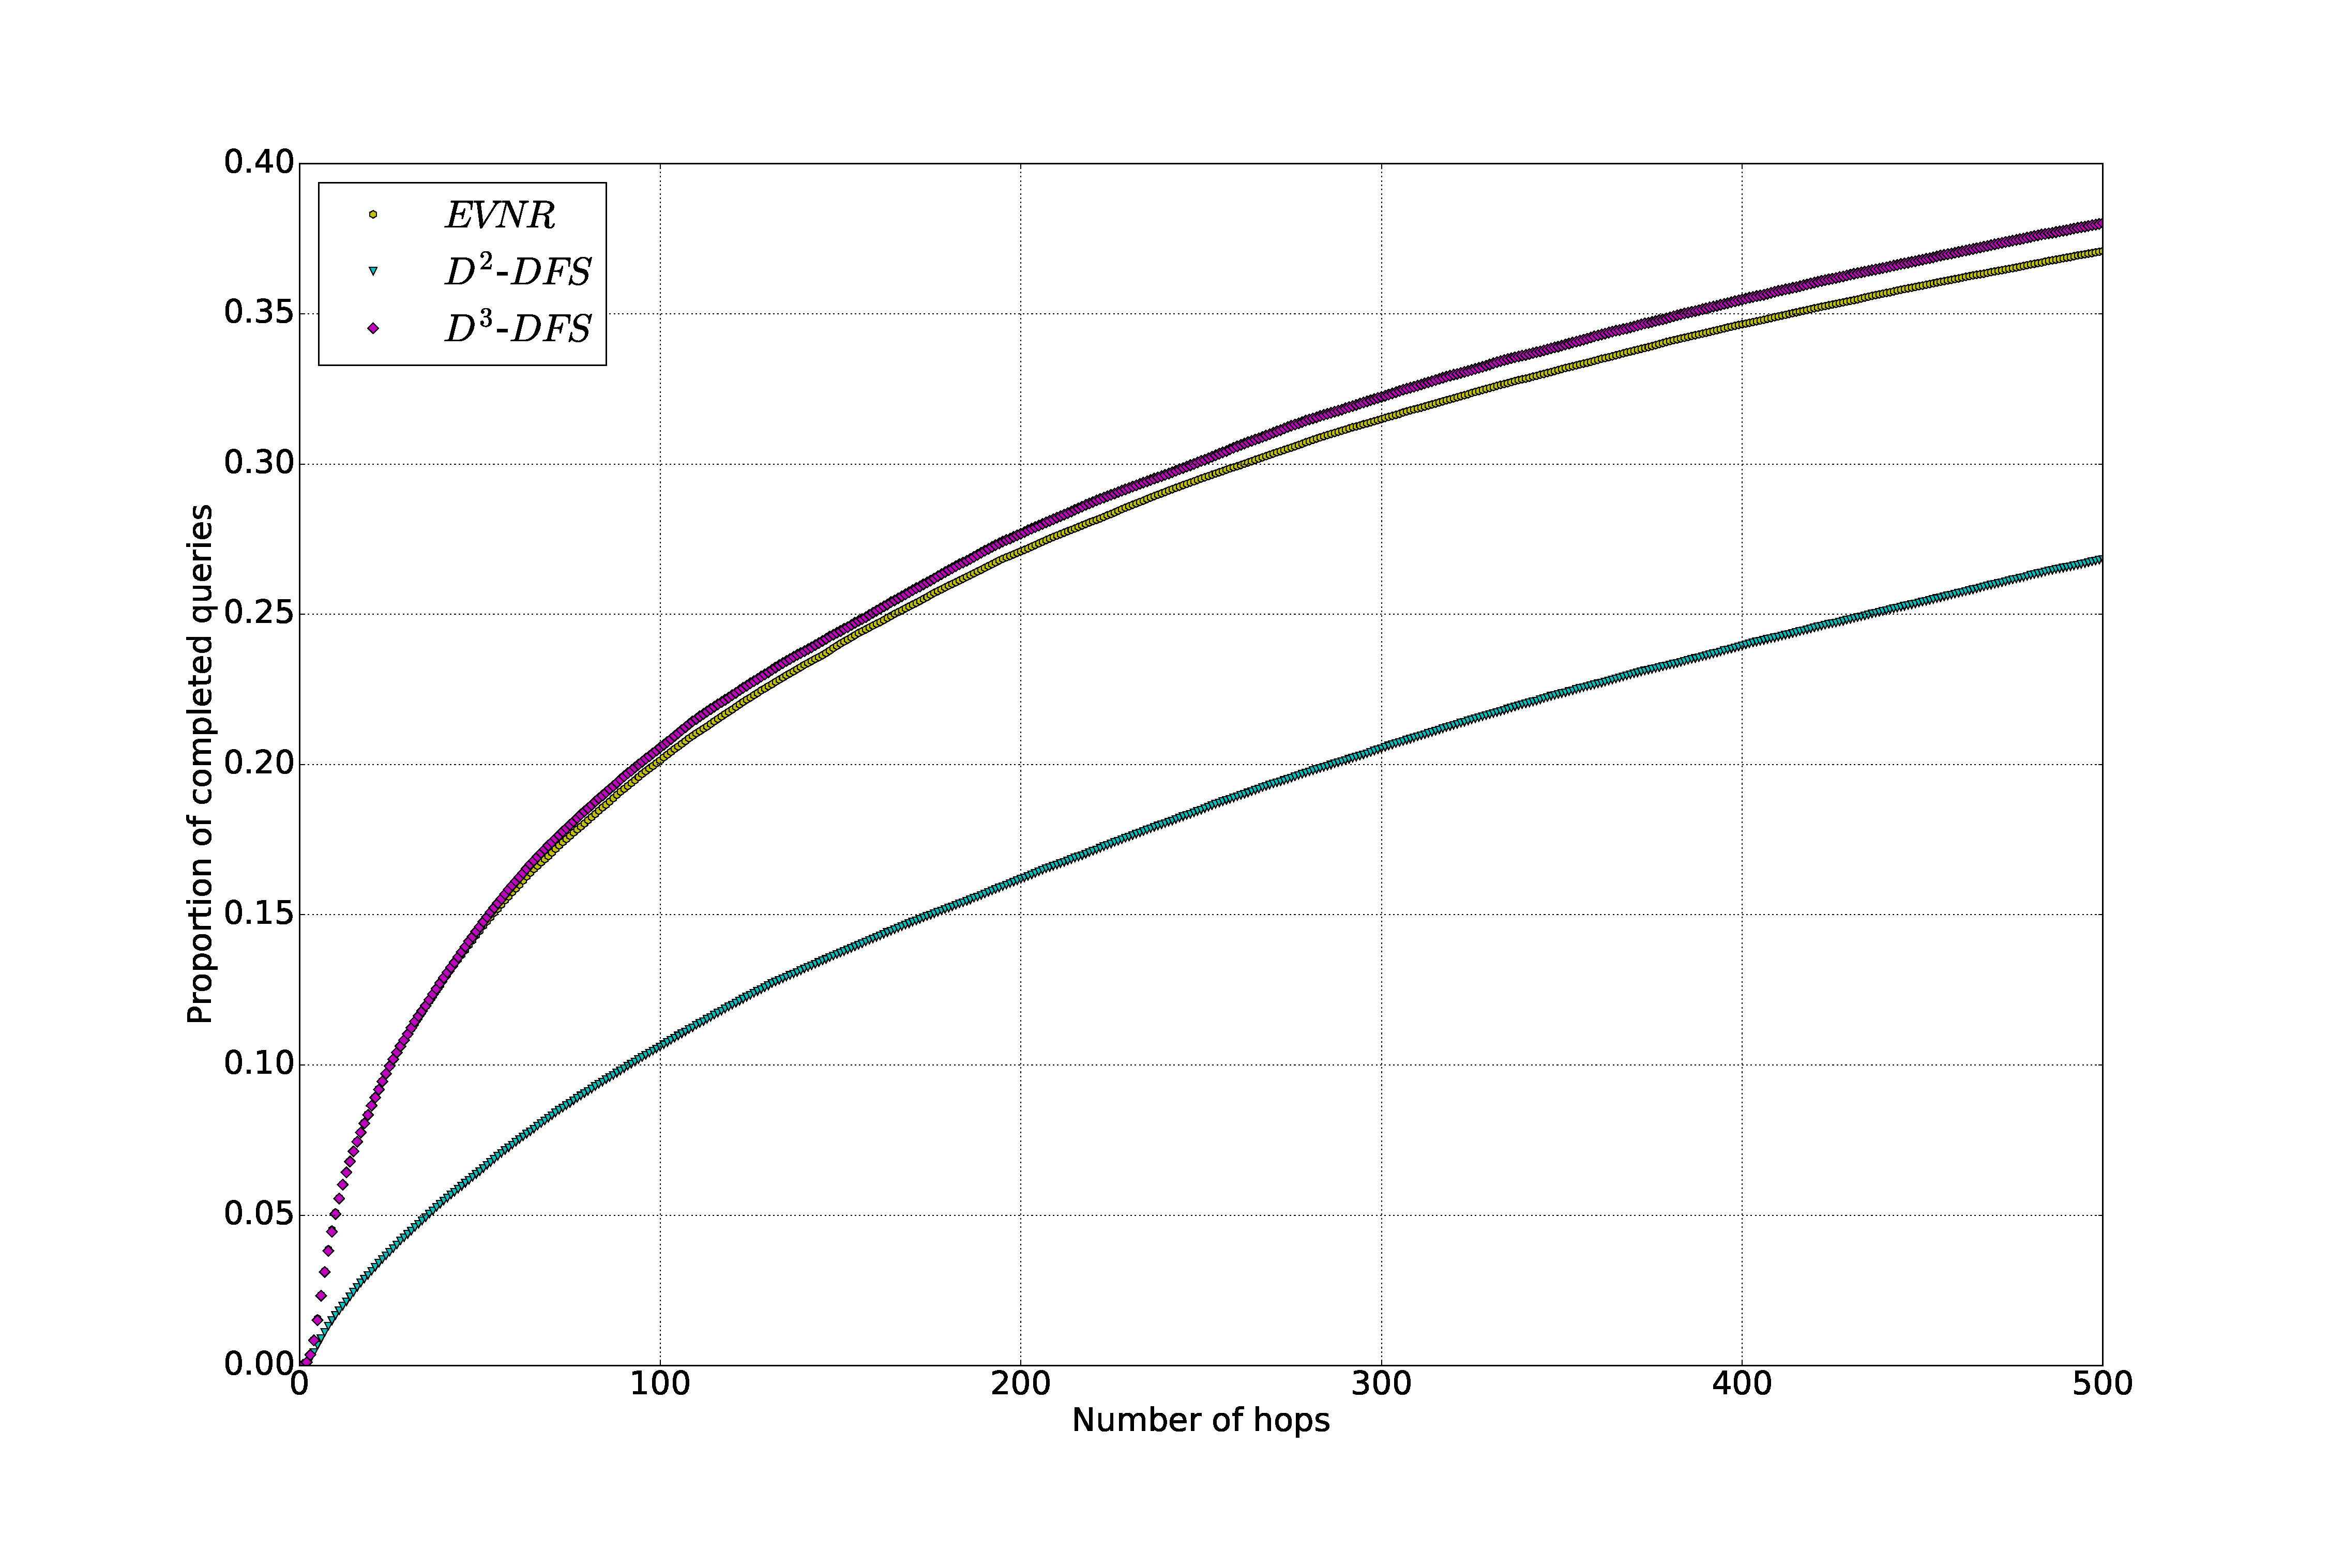
\includegraphics[width=47mm]{../fig/cml_100clip.eps}}
      \label{fig:41}
     \end{minipage}
    \end{center}

    \caption{次数上限を設定したWeb of Trustネットワークにおける \\ 各ホップ数以下で成功したルーティング試行の割合}
    \label{fig:cml_dclip}
   \end{figure}


\section{結論と今後の課題}
本研究ではF2Fネットワークにおける分散ルーティングの手法として主にFreenetのプロトコルを概観した. そしてSandbergの埋め込み生成アルゴリズムSWAPをWeb of Trustネットワークデータに適用し, ルーティングシミュレーションを行うことにより, $D^2$-$DFS$では$\log^2|V|$のホップ数上限のもとで20\%強という低い成功率と80強という決して短いとは言えない平均ホップ数しか達成できないことを実証的に確認した. よってFreenetの実装においてもOpennetを考慮しないピュアなF2Fモードではルーティングのパフォーマンスは低いことが予想できる.

その上で分散ルーティングの効率性を向上させるために $D^2$-$DFS$に隣接ノードの次数を考慮したヒューリスティックを加えた$D^3$-$DFS$を提案し, そのパフォーマンス評価を行った. 未処理のF2Fネットワークトポロジーデータ, 一部のハブノードを除いたデータ共に, $D^3$-$DFS$が$D^2$-$DFS$を成功率や平均ホップ数の面で凌ぐことが確認できたため, Freenet等の実際にデプロイされているF2Fネットワークの実装に活用できる可能性が大いにある. 

しかし$D^3$-$DFS$といえども今回の実験では成功率が40\%弱であり, ノードの次数上限を設けた場合は30\%弱と, それ自体決して高い値とは言えない. また表\ref{table:wot_info}の通り今回用いたWeb of Trustネットワークにおける本来の平均最短経路長が6.60であるの対し, $D^3$-$DFS$の平均ホップ数は依然60以上と最適値には程遠い. P2Pネットワークへの応用を考えた場合, ノード間の通信効率を保証するためにも他ノード到達の成功率を高く保ちホップ数を抑えることは非常に重要であるため, これらのパフォーマンス指標をさらに向上させることが, ピュアなF2Fネットワークを実用的なレベルにまで押し上げるための今後の課題である. 例えば今回次ノード選択のヒューリスティックに\cite{simsek2008navigating}で提案されたものを用いたが, 更に高いパフォーマンスを発揮するヒューリスティックを今後模索すべきであろう. また今回埋め込みアルゴリズムは先行研究のSWAPをそのまま用いたが, \cite{roos2017balanced}, \cite{boguna2010sustaining}等greedyルーティングが効率的となる様々な埋め込みのアルゴリズムが他にも提案されている. よって他の埋め込みアルゴリズムを適用した後のネットワークにおいて$D^3$-$DFS$が更に良いパフォーマンスを発揮できるか否か検証するべきだろう.

F2Fネットワークは信頼のおけるノード間に限った通信という厳しい制約上, 効率面において未だ多くの問題を残している. しかし今後はF2Fの直面する安全性と効率性というトレードオフを解消し, F2Fの実用性向上に努めていきたい. 

最後に$D^3$-$DFS$アルゴリズムを仮にFreenetプロトコルに導入するとした場合, 今回のシミュレーション実験に加えて行うべきいくつかの検証項目について述べておく.

\subsubsection*{データのinsert/requestの評価}
本研究ではルーティングを「特定のノードの探索」というシンプルなタスクとして設定したが, Freenetで実際に行われるルーティングは若干異なり「特定のデータを持ったノードの探索」(request) もしくは「特定のデータを保持すべきノードの探索」(insert) である. よって今後は$D^3$-$DFS$を用いたinsertによってデータがネットワーク全体にどのように分布するか, また$D^3$-$DFS$を用いたrequestによって任意のノードから任意のデータに効率的に到達可能かを検証せねばならない. それによって今回提案したアルゴリズムがFreenetにおけるデータの送受信でどの程度のパフォーマンスを発揮できるかをより正確に知ることができるであろう. 

\subsubsection*{セキュリティ面の評価}
Freenetはその目的においてセキュリティレベルを高く保つ必要がある. $D^3$-$DFS$は既存のFreenetにおけるF2Fモードにはない「ノードの次数」という新しい情報を隣接ノード間で共有することにより実現が可能であり, 次数情報自体はグラフ全体のトポロジーや隣接ノード以外のアイデンティティを明らかにするものではないため, 仮に何らかの方法で悪意を持ったノードがFreenet上の特定ノードの信頼を得てネットワークに参加したとしても, 直接接続していないノードのプライバシー侵害を行ったりすることは不可能と考えられる. しかし既存のFreenetプロトコルにも言えることではあるが, 悪意のあるノードはリクエストを無視したり, あるいは意図的に次数の低い隣接ノードへリクエストをフォワードしたりといったDoS(denial-of-service)攻撃が可能なため, これがどの程度$D^3$-$DFS$のパフォーマンスに悪影響を及ぼすか等を検証すべきである.

\subsubsection*{Opennetノードの存在を考慮した評価}
実際のFreenetはピュアな今回の実験で想定したF2Fネットワークではなく, ネットワーク内に接続先を制限しないOpennetノードが多数存在している. よってOpennetノードが一定数存在する環境で$D^3$-$DFS$はどの程度パフォーマンスを向上させることができるか, もしくは$D^3$-$DFS$が効率的となるためにOpennetノードへどういったアルゴリズムでIDや次数を割り当てるべきかを検証する必要があるだろう. 

%% 謝辞 %%%%%%%%%%%%%%%%%%%%%%%%%%%%%%%%%%%%%%%%%%%%%%%%%%%%%%%%%%%%%%%%%%%%%%%%%
\acknowledgment
本研究に取り組むにあたって, 宮崎修次講師には研究のテーマの方向性, 手法等さまざまな側面において助言を下さったことに対し深く感謝の意を申し上げます. また研究会等で本研究に対する指摘, 助言をしてくださった同研究室の先生方, 先輩方, 同期の方々に御礼申し上げます.
%% 参考文献 %%%%%%%%%%%%%%%%%%%%%%%%%%%%%%%%%%%%%%%%%%%%%%%%%%%%%%%%%%%%%%%%%%%%%
\addcontentsline{toc}{section}{\refname} % 目次に参考文献を追加する.
                                         % chapter使用時は削除すること.

%% BibTeX 等を用いる場合は,上の thebibliography 環境を消してここに該当コードを
%% 挿入すること.
\bibliographystyle{ieeetr}
\bibliography{refs}


\clearpage
%% 付録 %%%%%%%%%%%%%%%%%%%%%%%%%%%%%%%%%%%%%%%%%%%%%%%%%%%%%%%%%%%%%%%%%%%%%%%%%
%% 付録は不要ならば削除してよい.
\appendix
\section{SWAPアルゴリズムにおける採択確率の導出}
   与えられたグラフ$G=(V,E)$のエッジがKleinbergモデルにおける式(\ref{eq:kleinberg_p})に基づいて生成されたと仮定した場合, 尤度関数$p(E|\phi)$は
   \begin{eqnarray*}
    p(E|\phi) = \prod_{(x,y) \in E}\frac{1}{d(\phi(x), \phi(y))^rZ}
   \end{eqnarray*}
   一方$p(\phi|E)$をエッジ集合$E$が観測された場合の$\phi$の事後分布とすれば, ベイズの定理によりこれを尤度関数を用いて書き直せて
   \begin{eqnarray*}
    p(\phi|E) &=&\cfrac{p(E|\phi)p(\phi)}{p(E)} \label{eq:posteri}
   \end{eqnarray*}
   よって$\phi_1$を現在のサンプル, $\phi_2$を候補サンプルとすれば, Metropolis-Hastingsアルゴリズムにおける採択確率$\beta(\phi_1,\phi_2)$は以下のように書き直せる. ただし提案分布$\alpha$はシンメトリックで$\alpha(\phi_1, \phi_2 ) = \alpha(\phi_2, \phi_1 )$を満たすとする. 
   \begin{eqnarray*}
    \beta (\phi_1, \phi_2) &=& \min \left[1, \cfrac{p(\phi_2|E)\alpha(\phi_2, \phi_1)}{p(\phi_1|E)\alpha(\phi_1, \phi_2)}\right] \\
                           &=& \min \left[1, \cfrac{p(\phi_2|E)}{p(\phi_1|E)}\right] \\
                           &=& \min \left[1, \cfrac{p(E|\phi_2)}{p(E|\phi_1)}\right] \\
    &=& \min \left[1, \prod_{(x,y) \in E}\cfrac{d(\phi_1(x), \phi_1(y))^r}{d(\phi_2(x), \phi_2(y))^r}\right] \\
   \end{eqnarray*}
ここで$\phi_2$を$\phi_1$においてある2つのノード$u,v \in V$のID割り当てを入れ替えたものとすれば, $\phi_1(x)=\phi_2 (y),\ \phi_1(y)=\phi_2 (x),\ \forall z \neq x, y,\ \phi_1(z)=\phi_2(z)$が成り立つから, $u,v$を含まないエッジの距離は無視することができて, 
\begin{eqnarray*}
     \beta(\phi_1, \phi_2)&=&\min \left[1, \frac{\prod_{w \in N(u)}d(\phi_1(w), \phi_1(u))^r\prod_{w \in N(v)}d(\phi_1(w), \phi_1(v))^r}{\prod_{w \in N(u)}d(\phi_2(w), \phi_2(u))^r\prod_{w \in N(v)}d(\phi_2(w), \phi_2(v))^r}\right] 
\end{eqnarray*}
Sandbergはパラメータ$r$を変えて数パターンのシミュレーション実験を行った結果, Kleinbergの解析的な結果と同じく$r$が空間の次元に一致する場合最もルーティングのパフォーマンスが良いことを示したため, Freenetの実装においても$r=1$と設定されている. 


%% 本文ここまで %%%%%%%%%%%%%%%%%%%%%%%%%%%%%%%%%%%%%%%%%%%%%%%%%%%%%%%%%%%%%%%%%
\fi
\ifoutputcover
\evenclearpage
%% 表紙,背表紙,提出用摘要 %%%%%%%%%%%%%%%%%%%%%%%%%%%%%%%%%%%%%%%%%%%%%%%%%%%%%
\makecover                      % 表紙
\makespine[1]                   % 背表紙([] 内は出力枚数)
\makeinsidecover                % 中表紙
\fi
\ifoutputabstractforsubmission
\makeabstractforsubmission      % 提出用摘要
\fi
\end{document}
